\newif\ifafour
\afourtrue

\RequirePackage[l2tabu,orthodox]{nag}
\ifafour 
  \documentclass[a4paper,14pt,oneside,openany,article]{memoir}
\else
  \documentclass[a5paper,10pt,twoside,openany,article]{memoir}
\fi

%!TEX root = ../dissertation.tex
\usepackage{etoolbox}
\usepackage{pdflscape}
\usepackage{geometry}
\usepackage{xparse}

%% Various maths
\usepackage{amsthm,amsmath,amscd,amsfonts,amssymb,mathtools,amsthm,systeme}
\DeclareMathOperator\erf{erf}
%% Localization
\usepackage[main=russian,german,english]{babel}
\usepackage{fontspec}
\usepackage{iflang}

% for external links
\usepackage{xr}
% \makeatletter
% \newcommand*{\addFileDependency}[1]{% argument=file name and extension
%   \typeout{(#1)}
%   \@addtofilelist{#1}
%   \IfFileExists{#1}{}{\typeout{No file #1.}}
% }
% \makeatother
% \newcommand*{\myexternaldocument}[1]{%
%     \externaldocument{#1}%
%     \addFileDependency{#1.tex}%
%     \addFileDependency{#1.aux}%
% }


\providecommand{\noopsort}[1]{}
%% Fonts
\setmonofont{Courier New}
\defaultfontfeatures{Ligatures=TeX}
\setmainfont{Times New Roman}
\setsansfont{Arial}

%% Page geometry
\geometry{a5paper, top=14mm, bottom=14mm, inner=18mm, outer=10mm, footskip=5mm, nomarginpar}
\setlength{\topskip}{0pt}
\setlength{\footskip}{12.3pt}
\SingleSpacing

\makeevenhead{plain}{}{\thepage}{}
\makeoddhead{plain}{}{\thepage}{}
\makeevenfoot{plain}{}{}{}
\makeoddfoot{plain}{}{}{}
\pagestyle{plain}

%% Penalties
\tolerance=1414
\hbadness=1414
\emergencystretch=1.5em
\hfuzz=0.3pt
\vfuzz=\hfuzz
\clubpenalty=10000
\widowpenalty=10000
\brokenpenalty=4991

% \usepackage{totcount}
% \usepackage{lastpage}
% \regtotcounter[auxfile=totals.aux]{figure}
% \regtotcounter[auxfile=totals.aux]{table}
% \regtotcounter[auxfile=totals.aux]{page}
% \regtotcounter[auxfile=totals.aux]{algorithm}
% \newtotcounter[auxfile=totals.aux]{citnum}
% \newtotcounter[auxfile=totals.aux]{appendix}

%% Tuning of Table of Contents
\renewcommand{\cftchapterdotsep}{\cftdotsep}
\setrmarg{2.55em plus1fil}
\renewcommand{\cftchapterpagefont}{\normalfont}
\renewcommand{\cftchapterleader}{\cftdotfill{\cftchapterdotsep}}

% вот это чтобы были точки после номеров глав и подглав в содержании:
\renewcommand{\cftchapteraftersnum}{.\space}
\renewcommand{\cftsectionaftersnum}{.} 
\renewcommand{\cftsubsectionaftersnum}{.}

% чтобы были точки после номеров подразделов в тексте диссера
\AtBeginDocument{\setsecnumformat{\csname the#1\endcsname.~}}
\renewcommand*{\cftappendixname}{\appendixname\space}

%% Tuning of List of Figures/Tables
\makeatletter
\renewcommand{\@tocrmarg}{4em}
\renewcommand{\@pnumwidth}{3em}
\makeatother

%% Fonts and intervals of the basic things
%% Вот это задает отступы сверху и снизу от заголовкой и под-заголовков.
\newcommand{\basegostsectionfont}{\fontsize{10pt}{12pt}\selectfont\bfseries}
\newlength{\gostindent}
\setlength{\gostindent}{15pt}
% \setbeforesecskip{\gostindent}
% \setaftersecskip{\gostindent}
% \setbeforesubsecskip{\gostindent}
% \setaftersubsecskip{\gostindent}
% \setbeforesubsubsecskip{\gostindent}
% \setaftersubsubsecskip{\gostindent}

\makechapterstyle{thesisgost}{%
\chapterstyle{default}%
\setlength{\beforechapskip}{0pt}%
\setlength{\midchapskip}{0pt}%
\setlength{\afterchapskip}{\gostindent}%
\renewcommand*{\chapnamefont}{\basegostsectionfont}%
\renewcommand*{\chapnumfont}{\basegostsectionfont}%
\renewcommand*{\chaptitlefont}{\basegostsectionfont}%
\renewcommand*{\chapterheadstart}{}%
 \renewcommand*{\afterchapternum}{\quad}% <noscode> Ставит пробел между номером главы и названием в тексте, если закомментировать, то будет перенос строки
\renewcommand*{\printchapternum}{\centering\chapnumfont\thechapter}%
\renewcommand*{\printchaptername}{}%
\renewcommand*{\printchapternonum}{\centering}}

\makeatletter
\makechapterstyle{thesisgostchapname}{%
    \chapterstyle{thesisgost}
    \renewcommand*{\printchapternum}{\chapnumfont \thechapter .}   % точка после номера главы в тексте
    \renewcommand*{\printchaptername}{\centering\chapnamefont\@chapapp} %
}
\makeatother

\chapterstyle{thesisgost}
\setsecheadstyle{\basegostsectionfont\centering}
\setsecindent{0pt}
\setsubsecheadstyle{\basegostsectionfont\centering}
\setsubsecindent{0pt}
\setsubsubsecheadstyle{\basegostsectionfont\centering}
\setsubsubsecindent{0pt}
\sethangfrom{\noindent #1}

\chapterstyle{thesisgostchapname}
\renewcommand*{\cftchaptername}{\chaptername\space}

%% Making all the counters global
\counterwithout{equation}{chapter}
\counterwithout{equation}{section}
\counterwithout{equation}{subsection}
\counterwithout{figure}{chapter}
\counterwithout{figure}{section}
\counterwithout{figure}{subsection}
\counterwithout{table}{chapter}
\counterwithout{table}{section}
\counterwithout{table}{subsection}

\AtBeginDocument{%
\regtotcounter{totalcount@figure}%
\regtotcounter{totalcount@table}%
\regtotcounter{totalcount@algorithm}%
\regtotcounter{TotPages}%
}

%% Some not yet used magic to form Russian messages about sizes and counts
%% http://www.linux.org.ru/forum/general/6993203#comment-6994589 (используется totcount)
\makeatletter
\def\formbytotal#1#2#3#4#5{%
    \newcount\@c
    \@c\totvalue{#1}\relax
    \newcount\@last
    \newcount\@pnul
    \@last\@c\relax
    \divide\@last 10
    \@pnul\@last\relax
    \divide\@pnul 10
    \multiply\@pnul-10
    \advance\@pnul\@last
    \multiply\@last-10
    \advance\@last\@c
    \total{#1}~#2%
    \ifnum\@pnul=1#5\else%
    \ifcase\@last#5\or#3\or#4\or#4\or#4\else#5\fi
    \fi
}
\makeatother

%% A special environment for locale-dependent commands
%% Usage: \newlocalizedcommand{\YourCommandName}{expansion in English}{expansion in Russian}
%%        \renewlocalizedcommand{\YourCommandName}{expansion in English}{expansion in Russian}
\newcommand{\newlocalizedcommand}[3]{\newcommand{#1}{\IfLanguageName{russian}{#3}{#2}}}
\newcommand{\renewlocalizedcommand}[3]{\renewcommand{#1}{\IfLanguageName{russian}{#3}{#2}}}

%% Theorems (localized) %%
\newlocalizedcommand{\definitionname}{Definition}{Определение}
\newlocalizedcommand{\corollaryname}{Corollary}{Следствие}
\newlocalizedcommand{\theoremname}{Theorem}{Утверждение}
\newlocalizedcommand{\lemmaname}{Lemma}{Лемма}

\theoremstyle{definition}
\newtheorem{definition}{\definitionname}
\newtheorem{theorem}{\theoremname}
\newtheorem{lemma}{\lemmaname}
\newtheorem{corollary}{\corollaryname}

%% Paragraph formatting %%
\usepackage{indentfirst}
\AtBeginDocument{\setlength{\parindent}{2.5em}}

%% Enumerations (partially localized) %%
\usepackage{enumitem}
\setlist{nosep,labelindent=\parindent,leftmargin=*}

\makeatletter
\def\asbukx#1{\expandafter\@asbukx\csname c@#1\endcsname}
\def\@asbukx#1{\ifcase#1\or a\or б\or в\or г\or д\or е\or ж\or и\or к\or л\or м\or н\or п\or р\or с\or т\or у\or ф\or х\or ц\or ш\or щ\or э\or ю\or я\fi}
\def\Asbukx#1{\expandafter\@Asbukx\csname c@#1\endcsname}
\def\@Asbukx#1{\ifcase#1\or А\or Б\or В\or Г\or Д\or Е\or Ж\or И\or К\or Л\or М\or Н\or П\or Р\or С\or Т\or У\or Ф\or Х\or Ц\or Ш\or Щ\or Э\or Ю\or Я\fi}
\AddEnumerateCounter{\Asbukx}{\@Asbukx}{М}
\AddEnumerateCounter{\asbukx}{\@asbukx}{м}
\makeatother

\renewcommand{\labelitemi}{\normalfont\bfseries{--}}
\renewcommand\labelenumii{\arabic{enumii})}
\renewcommand\theenumii{\arabic{enumii}}
\renewlocalizedcommand{\labelenumi}{\alph{enumi})}{\asbukx{enumi})}
\renewlocalizedcommand{\theenumi}{\alph{enumi}}{\asbukx{enumi}}


%% Tuning of how floats look like
% We use floatrow/caption instead of memoir's poorly-working built-ins
\let\newfloat\undefined
\usepackage{caption}
\usepackage{floatrow}
\usepackage{subcaption}


%% Babel uses its own way to control captions, adhere to it
\addto{\captionsenglish}{%
\renewcommand{\figurename}{Figure}%
\renewcommand{\contentsname}{Contents}%
%\renewcommand{\ALG@name}{Algorithm}
}
\addto{\captionsrussian}{%
\renewcommand{\figurename}{Рисунок}%
\renewcommand{\contentsname}{Содержание}%
%\makeatletter
%\renewcommand{\ALG@name}{Листинг}%
%\makeatother
\renewcommand{\algorithmname}{Листинг}%
}

\floatsetup[figure]{style=plain, capposition=bottom}
\captionsetup[figure]{
    labelsep=endash,
    singlelinecheck=false,
    labelfont={normalsize,md},
    justification=centering,
    position=bottom
}
\floatsetup[table]{style=plain, capposition=top}
\captionsetup[table]{
    labelsep=endash,
    singlelinecheck=false,
    labelfont={normalsize,md},
    justification=justified,
    position=top
}
\floatsetup[algorithm]{style=plain, capposition=top}
\captionsetup[algorithm]{
    labelsep=endash,
    singlelinecheck=false,
    labelfont={normalsize,md},
    justification=justified,
    position=top
}

%\floatsetup[lstlisting]{style=plain, capposition=top}
%\captionsetup[lstlisting]{
%    labelsep=endash,
%    singlelinecheck=false,
%    labelfont={normalsize,md},
%    justification=justified,
%    position=top
%}

%% Tuning of table-of-contents

\settocdepth{subsection}            % до какого уровня подразделов выносить в оглавление
\setsecnumdepth{subsection}         % до какого уровня нумеровать подразделы

%% Custom math fonts

\usepackage{mathrsfs}

%% Graphics

\usepackage[dvipsnames, table, hyperref, cmyk]{xcolor}
\usepackage{graphicx}
\usepackage{pgfplots}
\pgfplotsset{compat=newest} 

% Include articles
\usepackage[final]{pdfpages}

%% Tables %%
\usepackage{tabularx}
\usepackage{longtable}
\usepackage{multirow,makecell}
\usepackage{hhline}
\usepackage{adjustbox}

\newcommand{\specialcell}[2][c]{%
  \begin{tabular}[#1]{@{}c@{}}#2\end{tabular}}

%% Hyperref %%
\usepackage{hyperref}
\definecolor{linkcolor}{rgb}{0,0,0}
\definecolor{citecolor}{rgb}{0,0,0}
\definecolor{urlcolor}{rgb}{0,0,0}

% No hypersetup here, as it needs some information not available here

%% Algorithmic environments %%
%\usepackage[linesnumbered,lined,boxed,commentsnumbered]{algorithm2e}
\usepackage{algorithm}
%\usepackage{algorithmic}
\usepackage[noend]{algpseudocode}
%\usepackage{amsmath}, amsthm,amsfonts,amssymb,amscd}

\algrenewcommand\algorithmicrequire{\textbf{Input:}}
\algrenewcommand\algorithmicensure{\textbf{Output:}}
\algnewcommand\algorithmicto{\textbf{to}}
\algrenewtext{For}[3] {\algorithmicfor\ $#1 \gets #2$ \algorithmicto\ $#3$ \algorithmicdo}
\algnewcommand\Continue{\textbf{continue}}
\algnewcommand\AndL{\textbf{and} }
\algnewcommand\OrL{\textbf{or} }
\algnewcommand\True{\textbf{True}}
\algnewcommand\False{\textbf{False}}

%% Counters
\usepackage[figure,table,algorithm]{totalcount}
\usepackage{totcount}
\usepackage{totpages}

%% Misc localization commands %%
\let\origle\le   \renewlocalizedcommand{\le}{\origle}{\leqslant}
\let\origleq\leq \renewlocalizedcommand{\leq}{\origleq}{\leqslant}
\let\origge\ge   \renewlocalizedcommand{\ge}{\origge}{\geqslant}
\let\origgeq\geq \renewlocalizedcommand{\geq}{\origgeq}{\geqslant}
\let\origtan\tan \renewlocalizedcommand{\tan}{\origtan}{\operatorname{tg}}
\let\origcot\cot \renewlocalizedcommand{\cot}{\origcot}{\operatorname{ctg}}
\let\origcsc\csc \renewlocalizedcommand{\csc}{\origcsc}{\operatorname{cosec}}
\let\origempty\emptyset \renewlocalizedcommand{\emptyset}{\origempty}{\varnothing}

%% Misc technical things %%
\newcommand{\resetfloatcounters}{%
\setcounter{figure}{0}%
\setcounter{table}{0}%
\setcounter{theorem}{0}%
\setcounter{lemma}{0}%
\setcounter{definition}{0}%
\setcounter{corollary}{0}%
\setcounter{footnote}{0}%
}

%% Bibliography packages and configuration

\usepackage{csquotes} % biblatex рекомендует его подключать. Пакет для оформления сложных блоков цитирования.

%%% Загрузка пакета с основными настройками %%%
\makeatletter
\usepackage[backend=biber,% движок
bibencoding=utf8,% кодировка bib файла
sorting=none,%nyt,% настройка сортировки списка литературы
style=gost-numeric,% стиль цитирования и библиографии (по ГОСТ)
language=autobib,% получение языка из babel/polyglossia, default: autobib % если ставить autocite или auto, то цитаты в тексте с указанием страницы, получат указание страницы на языке оригинала
autolang=other,% многоязычная библиография
clearlang=true,% внутренний сброс поля language, если он совпадает с языком из babel/polyglossia
defernumbers=true,% нумерация проставляется после двух компиляций, зато позволяет выцеплять библиографию по ключевым словам и нумеровать не из большего списка
sortcites=true,% сортировать номера затекстовых ссылок при цитировании (если в квадратных скобках несколько ссылок, то отображаться будут отсортированно, а не абы как)
movenames=false,% имена всегда в начале
maxbibnames=10,% показывать максимум 10 имен
]{biblatex}
\ltx@iffilelater{biblatex-gost.def}{2017/05/03}%
{%\toggletrue{bbx:gostbibliography}%
%\renewcommand*{\revsdnamepunct}{\addcomma}}{}
% <noscode> убрала addcomma чтобы не было запятых чежду last name и first name
\renewcommand*{\revsdnamepunct}{}}{}
\makeatother

% <noscode> замена точки с запятой на запятую при цитировании нескольких источников
\renewcommand*{\multicitedelim}{\addcomma\space}

\renewcommand*{\newblockpunct}{\addperiod\addnbspace---\space\bibsentence}

\DefineBibliographyStrings{english}{pages = {pp\adddot}}

\DefineBibliographyExtras{russian}{%
  \protected\def\bibrangedash{--\penalty\value{abbrvpenalty}}% almost unbreakable dash
  \protected\def\bibdaterangesep{\bibrangedash}%тире для дат
}
\DefineBibliographyExtras{english}{%
  \protected\def\bibrangedash{--\penalty\value{abbrvpenalty}}% almost unbreakable dash
  \protected\def\bibdaterangesep{\bibrangedash}%тире для дат
}

%Set higher penalty for breaking in number, dates and pages ranges
\setcounter{abbrvpenalty}{10000} % default is \hyphenpenalty which is 12
%Set higher penalty for breaking in names
\setcounter{highnamepenalty}{10000} % If you prefer the traditional BibTeX behavior (no linebreaks at highnamepenalty breakpoints), set it to ‘infinite’ (10 000 or higher).
\setcounter{lownamepenalty}{10000}

%% An environment which rewrites \cite to be \footfullcite for citations not in the author's list
\makeatletter
\newtoggle{footnotized@value}\togglefalse{footnotized@value}

\DeclareDocumentCommand{\trickycite}{oom}{%
\filteredcite{#3}%
\IfNoValueTF{#2}{%
\IfNoValueTF{#1}{%
% no #1 no #2
\iftoggle{footnotized@value}{\unspace\footfullcite{#3}}{\oldcite{#3}}%
}{%
% yes #1 no #2
\iftoggle{footnotized@value}{\unspace\footfullcite[#1]{#3}}{\oldcite[#1]{#3}}%
}}{
% yes #1 yes #2
\iftoggle{footnotized@value}{\unspace\footfullcite[#1][#2]{#3}}{\oldcite[#1][#2]{#3}}%
}}%
\newenvironment{footnotizeexcept}[1]{\begingroup%
\DeclareCiteCommand{\filteredcite}{}{\ifkeyword{#1}{\global\togglefalse{footnotized@value}}{\global\toggletrue{footnotized@value}}}{}{}%
\let\oldcite\cite\let\cite\trickycite}{\let\cite\oldcite\endgroup}
\makeatother

% make subfigure caption in russian
\renewcommand\thesubfigure{\asbuk{subfigure}}

%something for code listings
\usepackage{listings}

\usepackage{algorithm}
\usepackage{algpseudocode}

\algnewcommand\algorithmicforeach{\textbf{for}}
\algdef{S}[FOR]{For}[1]{\algorithmicforeach\ #1\ \algorithmicdo}

%\usepackage{fixltx2e}
\MakeRobust{\Call}

\usepackage{graphics}

\usepackage{mathrsfs}
%\usepackage{eufrak}
% USe other times new roman to have small caps
%\usepackage{fontspec}
%\setmainfont{TeX Gyre Termes}

\setlength {\marginparwidth }{2cm} 

%!TEX root = ../dissertation.tex

\usepackage{xpatch}% or use http://tex.stackexchange.com/a/40705
\def\makenamesetup{%
  \def\bibnamedelima{~}%
  \def\bibnamedelimb{ }%
  \def\bibnamedelimc{ }%
  \def\bibnamedelimd{ }%
  \def\bibnamedelimi{ }%
  \def\bibinitperiod{.}%
  \def\bibinitdelim{~}%
  \def\bibinithyphendelim{.-}}    
\newcommand*{\makename}[3]{\begingroup\makenamesetup\xdef#1{#2, #3}\endgroup}

\newbibmacro*{name:bold}[2]{%
  \makename{\currname}{#1}{#2}%
  \makename{\findname}{\lastname}{\firstname}%
  \makename{\findinit}{\lastname}{\firstinit}%
  \ifboolexpr{ test {\ifdefequal{\currname}{\findname}}
            or test {\ifdefequal{\currname}{\findinit}} }{\bfseries}{}}

\newcommand*{\boldname}[3]{%
  \def\lastname{#1}%
  \def\firstname{#2}%
  \def\firstinit{#3}}
\boldname{}{}{}

\xpretobibmacro{name:family}{\begingroup\usebibmacro{name:bold}{#1}{#2}}{}{}
\xpretobibmacro{name:given-family}{\begingroup\usebibmacro{name:bold}{#1}{#2}}{}{}
\xpretobibmacro{name:family-given}{\begingroup\usebibmacro{name:bold}{#1}{#2}}{}{}
\xpretobibmacro{name:delim}{\begingroup\normalfont}{}{}

\xapptobibmacro{name:family}{\endgroup}{}{}
\xapptobibmacro{name:given-family}{\endgroup}{}{}
\xapptobibmacro{name:family-given}{\endgroup}{}{}
\xapptobibmacro{name:delim}{\endgroup}{}{}

%%% This is a place to put all definitions needed for this particular thesis to work

% Various definitions depending on how the bibliography is done

\addbibresource{dissertation.bib}
\DeclareSourcemap{		
    \maps{
        \map{
            \step[fieldsource=medium, match=\regexp{Электронный\s+ресурс}, final]
            \step[fieldset=media, fieldvalue=eresource]
        }
    }
}

% Definitions and includes related for the text

% \DeclareRobustCommand{\todo}{\textcolor{black}}
\newcommand{\revise}[1]{\textcolor{red}{#1}}
\graphicspath{{images/}}

\newcommand{\hamm}[1]{\mathcal{H}(#1)}
\newcommand{\tobinary}[1]{\mathcal{B}(#1)}
\newcommand{\theop}{\mathcal{X}}

\DeclareMathOperator*{\argmin}{arg\,min}
\DeclareMathOperator*{\argmax}{arg\,max}

\pgfplotscreateplotcyclelist{myplotcycle}{%
black\\%1
red!80!black\\%2
violet!80!black\\%3
gray!80!black\\%4
orange\\%5
brown!80!black\\%6
cyan!80!black\\%
green!70!black\\%7
green\\%8
blue!60!black\\%9
teal\\%10
magenta!70!black\\%11
yellow!90!black\\%12
}


\DeclarePairedDelimiter\abs{\lvert}{\rvert}
\DeclarePairedDelimiter\ceil{\lceil}{\rceil}
\DeclarePairedDelimiter\floor{\lfloor}{\rfloor}
\definecolor{darkred}{rgb}{0.7,0.1,0.1}
\definecolor{middarkgrey}{rgb}{0.35,0.35,0.35}
\definecolor{darkblue}{rgb}{0.1,0.1,0.5}

\usepackage[colorinlistoftodos,prependcaption,textsize=tiny]{todonotes}
\usepackage[normalem]{ulem}
\usepackage{url}

\usepackage{tikz}
\usetikzlibrary{shapes,arrows, automata, positioning, arrows}
\usepackage{pstricks}
% \tikzset{
%   ->, % makes the edges directed
%   >=stealth', % makes the arrow heads bold
%   node distance=1.9cm, % specifies the minimum distance between two nodes. Change if necessary.
%   every state/.style={thick, fill=gray!10, minimum size = 0pt}, % sets the properties for each ’state’ node
%   initial text=$ $, % sets the text that appears on the start arrow
% }

% \newcommand{\inote}[1]{\medskip\noindent$[$\textcolor{darkred}{Илья}: \emph{\textcolor{middarkgrey}{#1}}$]$\medskip}
% \newcommand{\inote}[1]{\todo[linecolor=Plum,backgroundcolor=Plum!25,bordercolor=Plum,inline]{#1}}
\newcommand{\needtodo}[1]{\todo[linecolor=Red,backgroundcolor=Red!25,bordercolor=Red,inline]{#1}}

\newcommand{\inote}[1]{}
% \newcommand{\needtodo}[1]{}

\newcommand{\pto}{\mathrel{\ooalign{\hfil$\mapstochar$\hfil\cr$\to$\cr}}}
\newcommand{\chresults}[1]{\section*{Выводы по главе~#1}
\addcontentsline{toc}{section}{Выводы по главе~#1}
}
% \newcommand{\chresults}[1]{}
\newcommand{\insection}[1]{В \textbf{разделе~#1}}
\newcommand{\insectionen}[1]{In the \textbf{section~#1}}


% my definitions
% local definitions
\usepackage{xspace} % prevents eating spaces
\newcommand{\dadi}[0]{$\partial$a$\partial$i\xspace}
\newcommand{\moments}[0]{\textit{moments}\xspace}
\newcommand{\momentsLD}[0]{\textit{momentsLD}\xspace}
\newcommand{\momi}[0]{\textit{momi2}\xspace}
\newcommand{\fastsimcoal}[0]{\textit{fastsimcoal2}\xspace}
\newcommand{\stdpopsim}[0]{\textit{stdpopsim}\xspace}
\newcommand{\demes}[0]{\textit{demes}\xspace}
\newcommand{\gadma}[0]{GADMA\xspace}

\renewcommand{\v}{\relax\ifmmode\expandafter\boldsymbol\else\expandafter\textv\fi} % vector
\newcommand{\m}{\expandafter\mathbf} % matrix


% scale math mode
\newcommand\scalemath[2]{\scalebox{#1}{\mbox{\ensuremath{\displaystyle #2}}}}

% tablenotes
\usepackage[flushleft]{threeparttable}

% start section after all figures and tables of previous section
\usepackage{placeins}  % \FloatBarrier

% P is centered column in table with sizes
\newcolumntype{P}[1]{>{\centering\arraybackslash}p{#1}}

% define new chi that is located inline
\DeclareRobustCommand{\rchi}{{\mathpalette\irchi\relax}}
\newcommand{\irchi}[2]{\raisebox{\depth}{$#1\chi$}} % inner command, used by \rchi
%!TEX root = ../dissertation.tex

\newcommand{\thesisSpecialtyNumber}{1.2.2}
\newlocalizedcommand{\thesisSpecialtyName}{Mathematical modeling, numerical methods and software packages (Engineering)}{«Математическое моделирование, численные методы
и комплексы программ (технические науки)»}
%\newcommand{\thesisSpecialtyNumberOld}{05.13.18}
%\newlocalizedcommand{\thesisSpecialtyNameOld}{?}{«Математическое моделирование, численные методы и комплексы программ»}
\newlocalizedcommand{\thesisAuthorFull}{Noskova Ekaterina Eduardovna}{Носкова Екатерина Эдуардовна}
\newlocalizedcommand{\thesisAuthorShort}{Noskova~E.~E.}{Носкова~Е.~Э.}
\newlocalizedcommand{\thesisDegreeGenitive}{PhD in Engineering}{кандидата технических наук}
\newlocalizedcommand{\thesisTitle}
{Methods for inferring demographic history models}
{Методы построения моделей демографических историй}

\newcommand{\thesisOrganizationEng}{ITMO University}
\newlocalizedcommand{\thesisOrganizationNominative}{\thesisOrganizationEng}{Национальный исследовательский университет ИТМО\\(Университет ИТМО)}
\newlocalizedcommand{\thesisOrganizationLocative}  {\thesisOrganizationEng}{Университете ИТМО}
\newlocalizedcommand{\thesisOrganizationGenitive}  {\thesisOrganizationEng}{Университета ИТМО}
\newlocalizedcommand{\thesisOrganizationShortGenitive}{ITMO University}{Университета~ИТМО}
\newlocalizedcommand{\thesisOrganizationLogo}{
\includegraphics[width=0.28\linewidth]{logo_en}}{
\includegraphics[width=0.35\linewidth]{logo_ru}}

\newlocalizedcommand{\thesisInTheLibrary}{in the library of \thesisOrganizationGenitive}{в библиотеке \thesisOrganizationGenitive}
\newlocalizedcommand{\thesisLibraryAddress}{49 Kronversky pr., Saint Petersburg, Russia}{197101, Санкт-Петербург, Кронверкский пр., д.49}
\newcommand{\thesisURLAddress}{\url{***}}

\newcommand{\thesisYear}{2023}
\newlocalizedcommand{\thesisCity}{Saint Petersburg}{Санкт-Петербург}
\newlocalizedcommand{\defenceDateTime}{\revise{on DD.MM.YYYY at HH:MM}}{\revise{DD.MM.YYYY в HH:MM}}
\newlocalizedcommand{\defenceAddress}{\revise{address, room number}}{\revise{адрес, аудитория}}

\newcommand{\defenceCouncilNumber}{02.18.00}
\newlocalizedcommand{\defenceCouncilAddress}{49 Kronversky pr., Saint Petersburg, Russia, room \revise{XXX}}{197101, Санкт-Петербург, Кронверкский пр., д.49, аудитория \revise{XXX}}
\newlocalizedcommand{\defenceCouncilSecretaryFull}{Mouromtsev Dmitry Ilich}{Муромцев Дмитрий Ильич}
\newlocalizedcommand{\defenceCouncilSecretaryDegree}{Doctor of Philosophy}{канд. техн. наук}
\newcommand{\defenceCouncilSecretarySignature}{\includegraphics[width=2cm]{secretary-signature.png}}

\newlocalizedcommand{\supervisorFull}{Ulyantsev Vladimir Igorevich}{Ульянцев Владимир Игоревич}
\newlocalizedcommand{\supervisorShort}{Ulyantsev~V.~I.}{Ульянцев~В.~И.}
\newlocalizedcommand{\supervisorDegree}{Doctor of Philosophy}{канд. техн. наук}

% \newlocalizedcommand{\opponents}
% {\textbf{Tulupyev Alexander L'vovich},\par
%  \revise{Doctor of Physical and Mathematical Sciences},\par
%  Professor of Informatics Department\par
%  Federal State Budgetary Educational Institution of\par 
%  Higher Professional Education \par 
%  "Saint-Petersburg State University"\par
%  \vspace{1ex}\par
%  \textbf{Pavel Bernard Brazdil},\par
%  Doctor of Philosophy,
%  Professor of Engineer Faculty, 
%  Senior Researcher of INESC TEC’s 
%  Laboratory of Artificial Intelligence and Decision Support,
%  University of Porto, Porto, Portugal
% }{\textbf{Тулупьев Александр Львович},\par
%  доктор физико-математических наук, \par
%  профессор кафедры информатики\par
%  федерального государственного бюджетного\par
%  образовательного учреждения высшего \par
%  профессионального образования\par
%  "Санкт-Петербургский государственный университет"\par
%  \vspace{1ex}\par
%  \textbf{Pavel Bernard Brazdil},\par
%  Doctor of Philosophy,
%  Professor of Engineer Faculty, 
%  Senior Researcher of INESC TEC’s 
%  Laboratory of Artificial Intelligence and Decision Support,
%  University of Porto, Porto, Portugal
% }

\newcommand{\nociteallauthorpublications}{\nocite{
noskova2020gadma,
noskova2023gadma2,
noskova2023bayesian,
zhernakova2020genome,
nikolic2022stepping,
adrion2020community,
lauterbur2023expanding,
gower2022demes}}

% noscode
% Some of my papers had very long lists of authors so I had to short them for synopsis, however, I do not want to use those papers in the main document
\newcommand{\nociteallauthorpublicationsmaindocument}{\nocite{
noskova2020gadma,
noskova2023gadma2,
noskova2023bayesian,
zhernakova2020genome,
nikolic2022stepping,
adrion2020community,
lauterbur2023expanding,
gower2022demes}}

% Bibliography filters. As of now, they somewhat depend on which publications the author has.


\defbibfilter{thesisIndexed}{\keyword{labauthor:noskova}\and\keyword{phd:noskova}\and\not\keyword{index:vak}\and\(\keyword{index:wos}\or\keyword{index:scopus}\)}

\newlocalizedcommand{\textDissPubs}{Author's publications on the topic of the thesis}{Публикации автора по теме диссертации}
\newlocalizedcommand{\textOtherPubs}{Author's publications on other topics}{Публикации автора по другим темам}
\newlocalizedcommand{\textRangeIndexed}{Publications indexed in Web of Science or Scopus}{Публикации в зарубежных изданиях, индексируемых в базах цитирования Web of Science или Scopus}
\newlocalizedcommand{\textRangeVak}{Publications indexed in Russian journal included in the List of the Higher Attestation Commission}{Публикации в журналах из перечня ВАК}
\newlocalizedcommand{\textRangeEtc}{Other publications (in Russian)}{Прочие публикации}
\newlocalizedcommand{\textProgram}{Registered computer programs}{Свидетельства о государственной регистрации программ для ЭВМ}

\defbibheading{headingDissIndexed}{\clearpage\chapter*{\textDissPubs}\section*{\textRangeIndexed}}

\newcommand{\printauthorpublications}{%
\printbibliography[filter=thesisIndexed,heading=headingDissIndexed]%
}

%\newcommand{\printauthorpublicationsappendix}{\printbibliography[filter=thesisAppendix,heading=headingAppendix]}
%% Common misc %%

\newlocalizedcommand{\textAsManuscript}{As a manuscript}{На правах рукописи}
\newlocalizedcommand{\textSpecialty}{Specialty}{Специальность}
\newlocalizedcommand{\textThesisFulfilsRequirementsOf}{A thesis submitted in fulfillment of the requirements for the degree of}{Диссертация на соискание учёной степени}
\newlocalizedcommand{\textSupervisorIs}{Scientific advisor:}{Научный руководитель:}
\newlocalizedcommand{\textSynopsis}{Synopsis}{Реферат}
\newlocalizedcommand{\textWorkDoneIn}{The research was carried out at}{Работа выполнена в}
\newlocalizedcommand{\textOpponentsAre}{Official opponents:}{Официальные оппоненты:}

%% Title page %%

\newcommand{\thetitlepage}{
\setcounter{page}{1}
\thispagestyle{empty}
% organization name
{\centering\thesisOrganizationNominative\par}
\vspace{0pt plus2fill}
% organization logo + permissions
\noindent\begin{tabularx}{\linewidth}{lXr}
\vspace{0pt}\thesisOrganizationLogo & & \textAsManuscript \\
\end{tabularx}\par
\vspace{0pt plus6fill}
% author
{\centering\large\thesisAuthorFull\par}
\vspace{0pt plus1fill}
% title + specialty
{\centering\textbf{\large\thesisTitle}\par
\vspace{0pt plus2fill}
%\textSpecialty\ \thesisSpecialtyNumberOld~---\par
%\thesisSpecialtyNameOld\par
\textSpecialty\ \thesisSpecialtyNumber~---\par
\thesisSpecialtyName\par
\vspace{0pt plus2fill}
\textThesisFulfilsRequirementsOf\par
\thesisDegreeGenitive\par}
\vspace{0pt plus4fill}
% supervisor
\begin{flushright}
\textSupervisorIs\par\supervisorDegree\par\supervisorFull
\end{flushright}
% place + date
\vspace{0pt plus4fill}
{\centering\thesisCity~--- \thesisYear\par}
\newpage
}

%% Synopsis heading misc %%

\newlocalizedcommand{\markupDissertationCouncilSignature}
{Scientific Secretary of the\par\thesisOrganizationShortGenitive\par Dissertation Council \defenceCouncilNumber,\par\defenceCouncilSecretaryDegree}
{Ученый секретарь\par диссертационного совета\par\thesisOrganizationShortGenitive\par\defenceCouncilNumber,\par\defenceCouncilSecretaryDegree}
\newlocalizedcommand{\markupDefenceWillBeAt}
{The defence will be held on \defenceDateTime~at the meeting of the \thesisOrganizationShortGenitive\ Dissertation Council \defenceCouncilNumber~at \defenceCouncilAddress.}
{Защита состоится \defenceDateTime~на~заседании диссертационного совета \thesisOrganizationShortGenitive\ \defenceCouncilNumber~по адресу: \defenceCouncilAddress.}
\newlocalizedcommand{\markupThesisAvailableAt}
{The thesis is available \thesisInTheLibrary, \thesisLibraryAddress, and on the Web at \thesisURLAddress.}
{С диссертацией можно ознакомиться \thesisInTheLibrary\ по адресу: \thesisLibraryAddress, а также на сайте \thesisURLAddress.}

%% Synopsis %%
\newcommand{\labelsyn}[1]{\label{#1}}
\newcommand{\thesynopsis}[4]{
\begin{otherlanguage}{#1}
%\setcounter{page}{1}
\begingroup
\let\extref\ref%
%\renewcommand*{\thepage}{#2.\arabic{page}}
\renewcommand*{\thefigure}{#2.\arabic{figure}}
\renewcommand*{\thetable}{#2.\arabic{table}}
\renewcommand*{\ref}[1]{\extref{syn:#2:##1}}%
\renewcommand*{\labelsyn}[1]{\label{syn:#2:##1}}%

% Если убрать footnotizeexcept и переставить refcextion (и закомментить тот что в preamble-pre.tex переписывает cite на footnotecite), то в рефератах ссылки будут идти на список литературы после диссертации, а не в сноски
% \begin{footnotizeexcept}{#3}
% \begin{refsection}    <----- было
\resetfloatcounters     % <---- стало
{\centering\Large\textbf{\textSynopsis}\addcontentsline{toc}{chapter}{\textSynopsis}\par}
\input{#4}
\begin{refsection}
\nociteallauthorpublications
\urlstyle{rm}\printauthorpublications\urlstyle{tt}
\newpage
\end{refsection} 
% \end{footnotizeexcept}

\endgroup
\end{otherlanguage}}

%% Some constants for hypersetup were not known until user data is defined

\hypersetup{
    unicode,
    linktocpage=true,
    plainpages=false,
    colorlinks,
    linkcolor={linkcolor},
    citecolor={citecolor},
    urlcolor={urlcolor},
    pdftitle={\thesisTitle},
    pdfauthor={\thesisAuthorShort},
    pdfsubject={\thesisSpecialtyNumber\ \thesisSpecialtyName},
    pdfkeywords={},
    pdflang={en}
}



\usepackage{filecontents}
\addbibresource{disseration.bib}

\DeclareBibliographyCategory{skipbibliography}
\DeclareCiteCommand{\myfootcite}[\mkbibfootnote]
  {\usebibmacro{prenote}}
  {\addtocategory{skipbibliography}{\thefield{entrykey}}%
   \usedriver
     {\DeclareNameAlias{sortname}{default}}
     {\thefield{entrytype}}}
  {\multicitedelim}
  {\usebibmacro{postnote}}

\begin{document}

% Основной текст диссертации
%\setcounter{page}{\value{savedpage}}

\section*{Обоснования для специальности 1.2.2}

\textbf{Актуальность темы исследования} обусловлена низкой эффективностью современных программных средств для решения задачи поиска демографической истории популяций по генетическим данным в области биоинформатики.

Популяция --- это группа особей одного вида, живущих на одной территории.
\textit{Демографическая история популяций} --- это история их развития и эволюции, которая включает в себя такие события как изменения численности популяций, разделения популяций, миграция и отбор.
Используя различные статистические и алгоритмические методы возможно ее реконструировать или вывести по генетическим данным.
Демографические истории используются для датирования исторических событий, не оставивших письменных свидетельств~\myfootcite{goebel2008late}\myfootcite{mellars2006going}, а также играют важную роль в области консервативной генетики~\myfootcite{nikolic2022stepping} и даже медицине~\myfootcite{nielsen2007recent}.

При поиске демографической истории популяции приходится прибегать к использованию модели --- параметрическому семейству демографических историй, которое позволяет ограничить пространство их поиска.
%Существует множество способов задать это параметрическое семейство.
%Из определения следует, что модель при каких-то значениях параметров является демографической историей.

Существует множество методов и программных решений для настройки значений параметров заданной модели по генетическим данным.
Эти методы включают в себя комбинацию алгоритмов численного моделирования и методов оптимизации.
На вход они требуют модель демографической истории, заданную пользователем (биоинформатиком или системным биологом) с использованием интерфейса выбранного программного решения, и осуществляют поиск оптимальных параметров этой модели.
Методы численного моделирования используются для вычисления функции правдоподобия демографической истории и данных.
Именно эта величина определяет оптимальность параметров и используется в качестве целевой функции в алгоритмах оптимизации.
Кроме того, подавляющее большинство методов использует алгоритмы локальной оптимизации для поиска параметров заданной модели.
Эти алгоритмы требуют определения начальных значений параметров и их эффективность зависит от этого выбора. 

Несмотря на наличие методов вывода демографической истории, выбор модели и начальных значений ее параметров все еще требуют ручной настройки и экспертных данных, что ограничивает получаемый результат.
Для улучшения точности и достоверности вывода, пользователь вынужден рассматривать множество возможных моделей, находить оптимальные значения параметров и сравнивать результаты между собой.
Рассматриваемые модели, в первую очередь, отличаются динамикой изменения численности популяций, тип которой всегда зафиксирован в модели.
При этом обычно используют три наиболее популярных динамики: константная численность, линейное или экспоненциальное изменение.
%Неверный выбор начальных оценок параметров моделей может снизить эффективность используемого алгоритма оптимизации и привести к недостоверным результатам при сравнении моделей.

Задача вывода демографической истории популяций дополнительно усложняется необходимостью реализации пользователем программного кода модели и алгоритма вывода ее параметров.
Методы численного моделирования, используемые существующими решениями, имеют разные возможности и стабильность работы, и пользователь может применить несколько из них для сравнения результатов.
Однако при использовании различных программных решений одновременно, пользователь сталкивается с необходимостью задавать одни и те же модели с использованием разных интерфейсов.

Таким образом, процесс вывода демографической истории требует значительных временных затрат, тем больших, чем больше рассматриваемых популяций, а также у пользователя опыта в области программирования и изучаемых видов.
Все это ограничивает возможности существующих подходов к выводу демографической истории популяций.\\
%Поэтому разработка новых методов, алгоритмов и программных средств для автоматического поиска демографической истории без заданной конфигурации модели является актуальной темой в области популяционной генетики.
%Такой подход может ускорить процесс вывода демографической истории популяций, повысить точность получаемых результатов и расширить возможности анализа генетических данных.\\

\newpage
В данной работе был разработан расширенный класс моделей, которые включают динамики изменения численности, как параметры для настройки моделей.
Программную реализацию разработанных моделей можно переиспользовать в программных решениях \dadi, \moments, \momentsLD, \momi для поиска демографической истории популяций.
После этого у пользователя больше не будет необходимости задавать несколько моделей, которые отличаются зафиксированными динамиками изменения численности, и прибегать к использованию разных интерфейсов.

Также в диссертации разработан метод настройки метод настройки параметров обобщенных моделей по генетическим данным.
Он является комбинацией существующих методов численного моделирования и глобальной оптимизации.
Автором было разработано два метода глобальной оптимизации. 
Первый основан на генетическом алгоритме и выполняет настройку моделей в случае одной двух и трех популяций.
Второй метод использует байесовскую оптимизацию для настройки моделей в случае более трех популяций.
Эти методы не требует начальных оценок параметров и позволяет эффективно находить глобальный оптимум.

Кроме того, в работе разработан метод автоматического выбора модели обобщенного класса и настройки ее параметров по генетическим данным. Этот алгоритм позволяет автоматически, без создания программного кода, перебирать модели обобщенного класса и выбирать ту, которая наилучшим образом описывает данные в заданных ограничениях.
На основе предложенных модели и методов автором создано соответствующее программное средство.

\subsection*{Обзор существующих решений для вывода демографической истории популяций}

Неформально говоря, демографическая история популяций --- это история развития и эволюции этих популяций, которая включает в себя информацию о дереве разделения популяций, численности популяций в прошлом, миграциях, отборе и многом другом.
В современной литературе строгого определения демографической истории нет.
Демографическая история может быть сколь угодно подробной, например, можно представить, что она описывает все геномы всех особей, которые когда-либо присутствовали в популяции или более того включает координаты перемещения этих особей по земному шару.
Однако, в современных исследованиях все же обычно не рассматривают настолько подробные объекты.
Вместо этого под демографической историей понимают историю разделения популяций, численности в каждый момент времени и темпы миграции.
В данной работе будут исследованы аналогичные объекты.
Опишем понятие демографической истории популяций, которое будет использовано в данной работе.
%поэтому определим некое множество объектов, которые будем называть демографической историей в данной работе.

Рассмотрим $P$ популяций.
Пусть имеется полное бинарное дерево с $P$ листьями, которое задает структуру разделения популяций.
Бинарное дерево называется полным, у каждого узла есть либо два дочерних элемента, либо ноль дочерних элементов.
Каждый лист дерева может быть ассоциирован с одной из текущих популяций, а остальные вершины --- популяциям в прошлом.
Например, вершина-родитель двух листьев, соответствующих популяциям 1 и 3, будет соответствовать их общей популяции, которая в какой-то момент в прошлом разделилась и образовала популяции 1 и 3.

\definition Дерево разделений $P$ популяций --- это полное бинарное дерево $T$, в котором множество листьев занумеровано числами от 1 до $P$.

Пример дерева разделений для четырех популяций изображен на рисунке~\ref{fig:dem_tree}.
Листья занумерованы числами от 1 до 4, которые соответсвуют номерам популяций.

\begin{figure}[h]
    \centering
    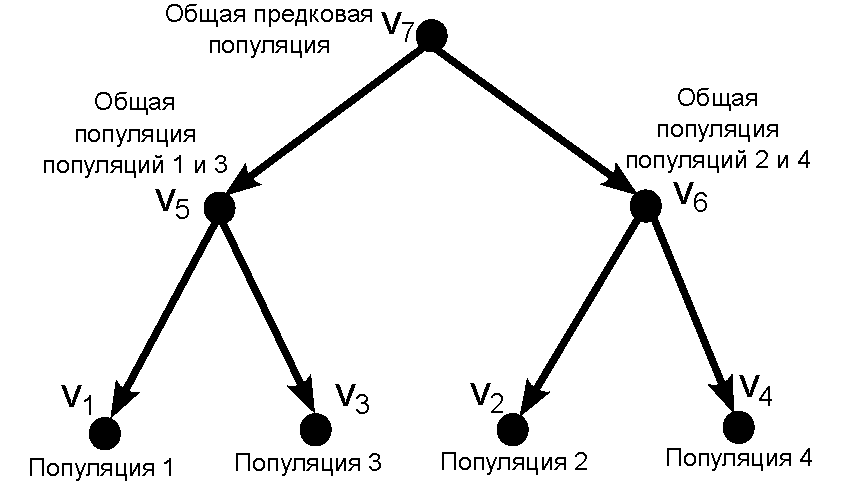
\includegraphics[width=0.6\textwidth]{images_2/dem_hist_tree.pdf}
    \caption{Пример дерева разделений популяций}
    \label{fig:dem_tree}
\end{figure}

Рассмотрим дерево разделений $P$ популяций.
Пусть для каждой популяции-вершины $v$ задано множество из времени образования $t_v \in \mathbb{R}_+$ этой популяции, времени ее разделения $t^d_v \in \mathbb{R}_+$ и функции изменения численности популяции $g(t): [t_v, t^d_v] \to \mathbb{R}_+$.
Время разделения популяции --- это время, когда она перестала существовать.
Заметим, что время образования каждой вершины, кроме корня, должно совпадать со временем разделения вершины-родителя.
Время отображается в поколениях в прошлом, поэтому $t^d_v < t_v$.
На функцию изменения численности никаких ограничений не накладывается, она не обязана быть непрерывной.
Пример дерева разделений с заданными временами образования и разделения популяций, а также функциями изменения численности изображен на рисунке~\ref{fig:dem_def}.


\begin{figure}[h]
    \centering
    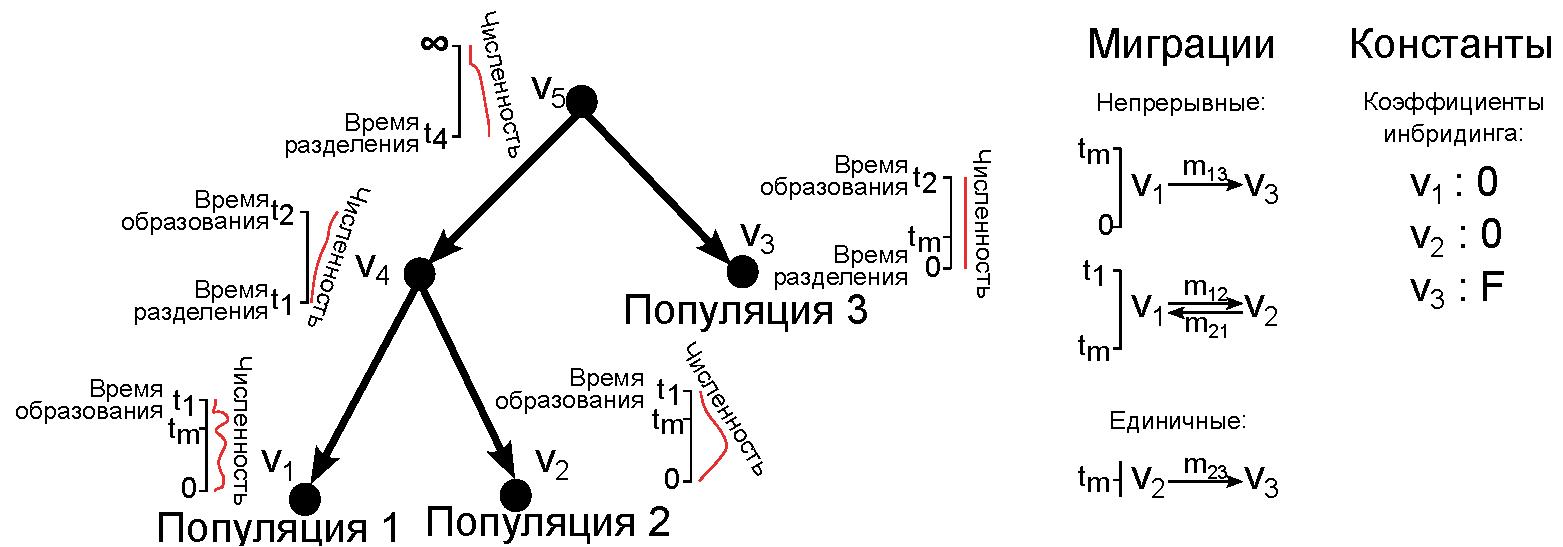
\includegraphics[width=0.7\textwidth]{images_2/dem_hist_def.pdf}
    \caption{Пример демографической истории популяций как дерева разделений с заданными временами образования и разделения популяций и функциями численности}
    \label{fig:dem_def}
\end{figure}

%Формальное определение демографической истории выглядит следующим образом:

\definition Демографическая история $\mathcal{D}$ для $P$ популяций --- двойка $<T, \mathfrak{G}>$, где $T = <V, E>$ --- дерево разделения популяций, $\mathfrak{G}: V \to \mathbb{R}_+ \times \mathbb{R}_+ \times \mathcal{F}_{\mathbb{R}_+ \to \mathbb{R}_+}$ --- отображение, которое для каждой вершины $v$ ставит в соответствие множество $<t_v, t^d_v, g(t)>$, где $t_v$ и $t^d_v$ --- время образования и разделения популяции соответственно, а функция $g(t): [t_v, t^d_v] \to \mathbb{R}_+$ определяет численность популяции в каждый момент ее существования.
На отображение $\mathfrak{G}$ накладывается следующее ограничение: для любой вершины $v$ время ее образования 
 $t_v$ равно времени разделения $t^d_{parent(v)}$ ее вершины-родителя.

Демографическую историю можно изображать различными способами.
Например, рисунок~\ref{fig:dem_def} является примером упрощенного визуального представления.
В данной работе будет использоваться представление, которое было предложено в работе~\myfootcite{gower2022demes}.

\begin{figure}[h]
    \centering
    \begin{subfigure}[b]{.33\textwidth}
    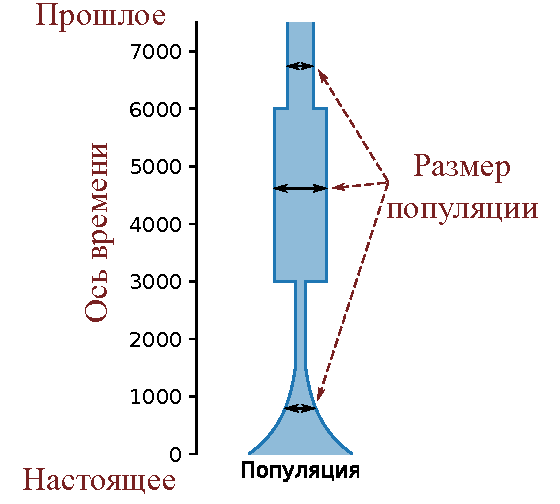
\includegraphics[width=\textwidth]{images/part1/dem_history/1d_model_fixed.pdf}
    \caption{}
    \label{fig:part1:dem_inf:dem_his_examples_1}
    \end{subfigure}%
    \begin{subfigure}[b]{.33\textwidth}
    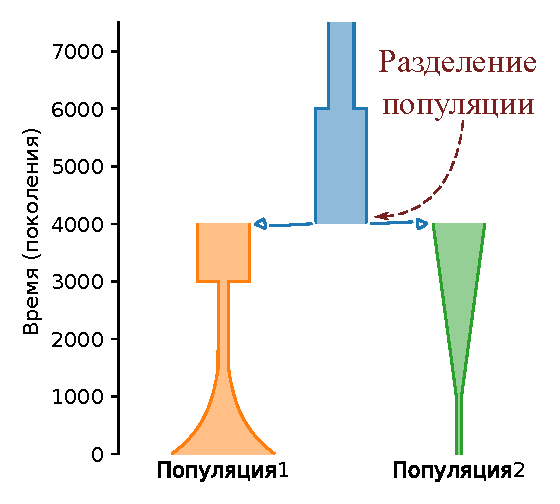
\includegraphics[width=\textwidth]{images/part1/dem_history/2d_model_isolation_fixed.pdf}
    \caption{}
    \label{fig:part1:dem_inf:dem_his_examples_2}
    \end{subfigure}%
    \begin{subfigure}[b]{.33\textwidth}
    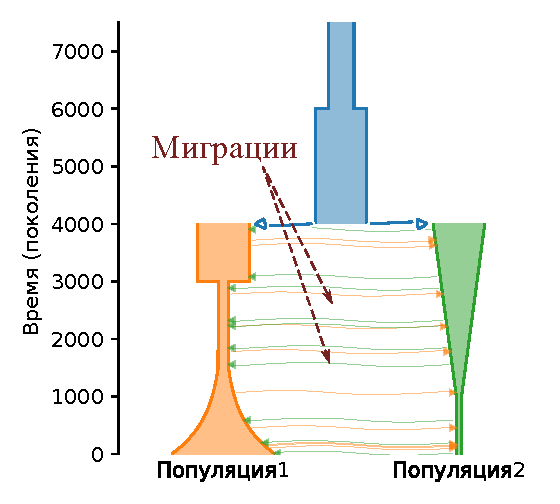
\includegraphics[width=\textwidth]{images/part1/dem_history/2d_model_migration_fixed.pdf}
    \caption{}
    \label{fig:part1:dem_inf:dem_his_examples_3}
    \end{subfigure}
    \caption{Примеры визуального представления демографических историй одной и двух популяций}
    \label{fig:part1:dem_inf:dem_his_examples}
\end{figure}

Примеры визуальных представлений демографических историй представлены на рисунке~\ref{fig:part1:dem_inf:dem_his_examples}. 
На рисунке~\ref{fig:part1:dem_inf:dem_his_examples_1} представлена демографическая история одной популяции, на рисунке~\ref{fig:part1:dem_inf:dem_his_examples_2}  --- демографическая история двух популяций без миграции, на рисунке~\ref{fig:part1:dem_inf:dem_his_examples_3} --- демографическая история двух популяций с миграцией.
Ось абсцисс соответствует числу поколений в прошлом, ноль --- настоящее время.
Время в демографических историях измеряется в поколениях, так как в процессе эволюции генетический материал передается от одного поколения к другому.
Как следует из изложенного выше, демографическая история --- древовидная структура.
Она, в частности, задает филогенетическое дерево популяций, которое отображает как популяции разделялись.
Однако демографическая история также содержит информацию о численности популяций и миграциях: это отображено шириной веток дерева и стрелками между ними.
Ширина раскрашенных областей соответствует размеру популяции в конкретный момент времени, а число стрелок зависит от степени миграций между популяциями.

Задача вывода демографической истории популяций по генетическим данным состоит в поиске наилучшей демографической истории из всего множества возможных историй.
Для сравнения демографических историй используется метрика правдоподобия, которая определяет насколько хорошо история описывает генетические данные.
Таким образом, задача состоит в поиске демографической истории с наибольшим значением правдоподобия для данных.
Напомним, что демографическая история включает в себя функции изменения численности, и поэтому, поиск по всему пространству возможных историй --- это, в том числе, и поиск по пространству функций, что вызывает трудности.

В результате, для упрощения задачи поиска ограничивают пространство рассматриваемых демографических историй.
Для этого используются параметрические модели или просто модели.
Приведем два эквивалентных определения параметрической модели демографической истории популяций.

\definition Параметрическая модель демографической истории --- это множество $\{\mathcal{D}_\theta\}_{\theta \in \Theta}$ демографических историй популяций, параметризованное набором параметров $\theta$.

\definition Параметрическая модель демографической истории --- отображение $f: \Theta \to \{\mathcal{D}\}$, которое любому набору значений параметров $\theta$ модели ставит в соответствие демографическую историю популяций $\mathcal{D}_\theta$.\\

Приведем пример модели демографической истории.
Пусть задана одна популяция и известно, что ее численность всегда была постоянна.
Все демографические истории одной популяции имеют одинаковое дерево разделений, состоящее из одной вершины.
Таким образом, все демографические истории одной популяции отличаются только функцией изменения численности.

Зная, что численность популяции постоянна, можно задать модель $M_1$ с одним параметром $\theta = (\theta_1)$, который будет соответствовать константному размеру популяции.
Таким образом, модель будет отображать пространство параметров в демографические популяции, у которой функция изменения численности будет равна $g(t) = \theta_1$.
Пример описанной модели $M_1$ представлен на рисунке~\ref{fig:model_def}.
На рисунке~\ref{fig:model_def_1} показано отображение из пространства параметров в множество демографических историй.
Рисунок~\ref{fig:model_def_2} демонстрирует визуальное изображение модели демографической истории, которое будет использовано в данной работе.
На рисунке представлено изображение демографической истории и схематично указано какую характеристику демографической истории регулирует параметр $\theta_1$.
Для того, чтобы продемонстрировать, что это не одна демографическая история, а множество, изображение модели дополнительно содержит пунктирные линии.

\begin{figure}[h]
    \centering
    \begin{subfigure}[b]{.59\textwidth}
    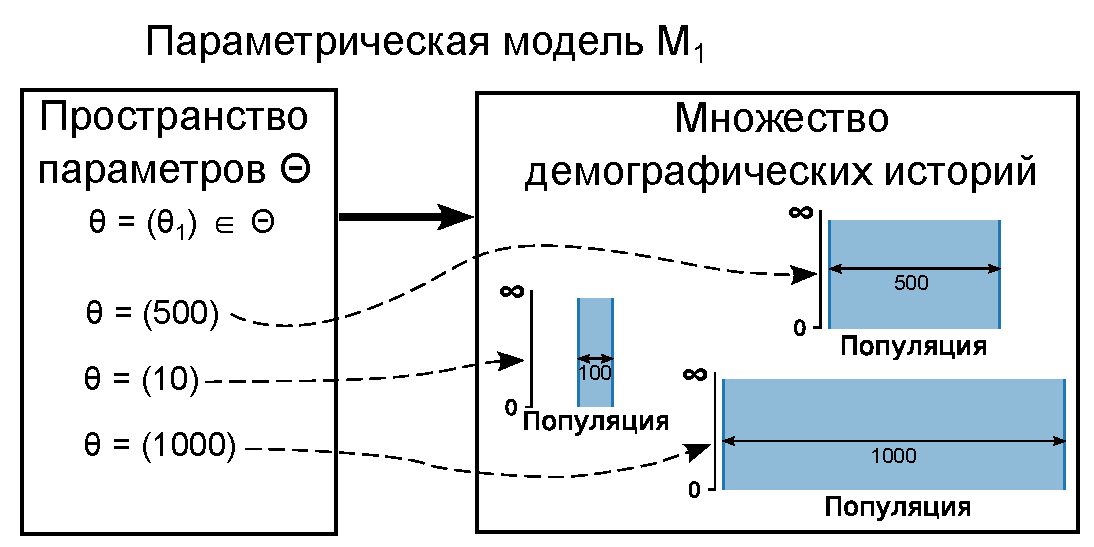
\includegraphics[width=\textwidth]{images_2/model_def.pdf}
    \caption{}
    \label{fig:model_def_1}
    \end{subfigure}%
    \begin{subfigure}[b]{.40\textwidth}
    \centering
    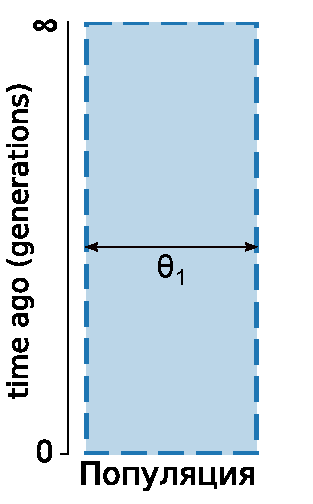
\includegraphics[width=0.45\textwidth]{images_2/model_pict.pdf}
    \caption{}
    \label{fig:model_def_2}
    \end{subfigure}
    \caption{Пример модели $M_1$ демографической истории одной популяции с одним параметром}
    \label{fig:model_def}
\end{figure}


Одни и те же параметры модели могут задавать разные характеристики демографических историй.
Например, на рисунке~\ref{fig:model_def2} представлена модель $M_2$, имеющая четыре параметра.
Эта модель представляет множество демографических историй одной популяции, у которых функция изменения численности определяется следующим образом:
$$
g(t) = 
\begin{cases}
    \theta_1, & \text{ если } t \leq \theta_3, \\
    \theta_2, & \text{ если } \theta_3 \leq t \leq \theta_3 + \theta_4, \\
    \theta_2, & \text{ если } t \geq \theta_3 + \theta_4.
\end{cases}
$$

Рисунок~\ref{fig:model_def2_1} изображает модель $M_2$ как отображение из пространства параметров в множество
демографических историй.
Рисунок~\ref{fig:model_def2_2} демонстрирует визуальное изображение модели.

Модель $M_2$ описывает демографическую историю с тремя периодами константной численности, при этом параметр $\theta_1$ задает и численность до момента времени $\theta_3 + \theta_4$, и после времени $\theta_3$.

\begin{figure}[h]
    \centering
    \begin{subfigure}[b]{.59\textwidth}
    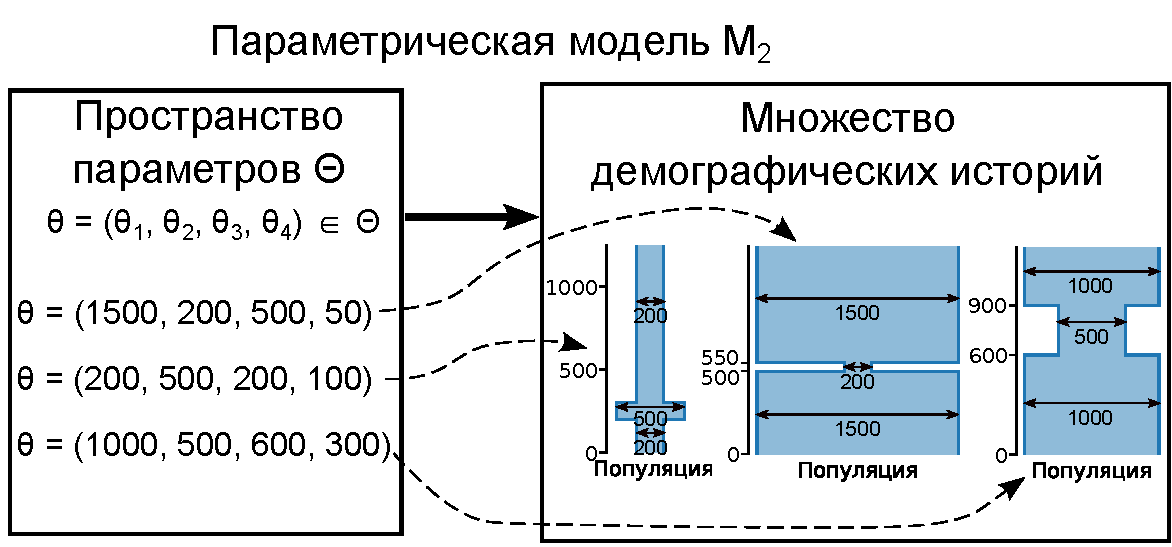
\includegraphics[width=\textwidth]{images_2/model_def_2.pdf}
    \caption{}
    \label{fig:model_def2_1}
    \end{subfigure}%
    \begin{subfigure}[b]{.40\textwidth}
    \centering
    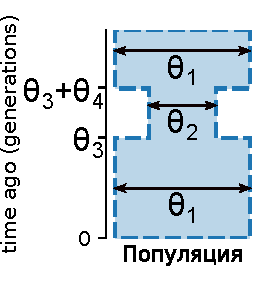
\includegraphics[width=0.6\textwidth]{images_2/model_pict_2.pdf}
    \caption{}
    \label{fig:model_def2_2}
    \end{subfigure}
    \caption{Пример модели $M_2$ демографической истории одной популяции с четырьмя параметрами}
    \label{fig:model_def2}
\end{figure}

Заметим, что множество демографических историй, определенных моделью $M_1$, вложено в множество историй, определенное моделью $M_2$ (рисунок~\ref{fig:nested_models}).
Тогда будем говорить, что модель $M_1$ является вложенной  в модель $M_2$. 

\begin{figure}[h]
    \centering
    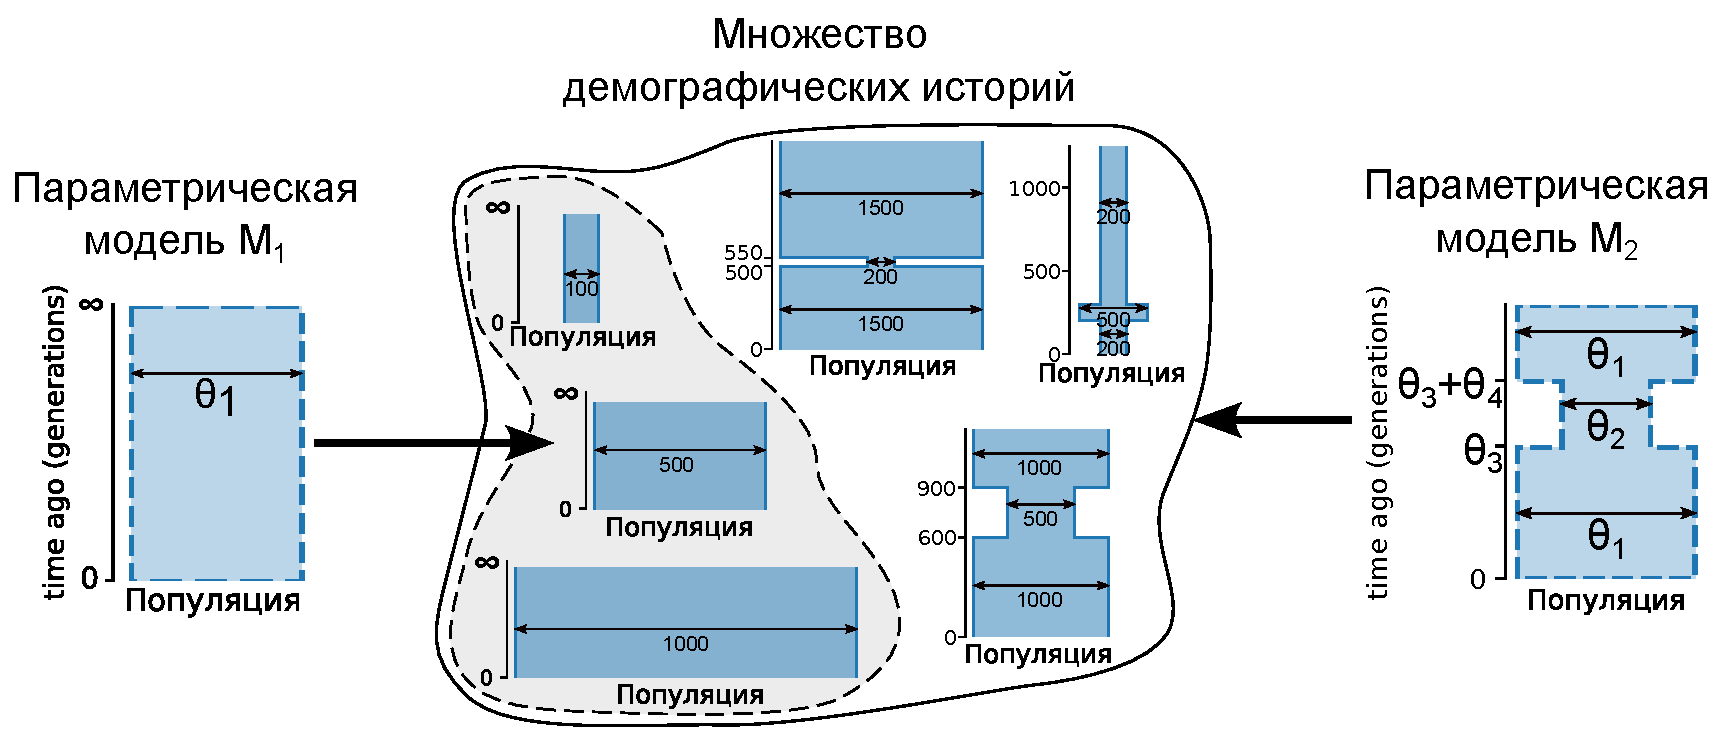
\includegraphics[width=\textwidth]{images_2/nested_models.pdf}
    \caption{Пример вложенных моделей: модель $M_1$ вложена в модель $M_2$}
    \label{fig:nested_models}
\end{figure}

Модели не всегда вложены друг в друга, иногда их множества демографических историй просто пересекаются.
Как следствие, одна и та же демографическая история может соответствовать разным моделям.

Вернемся к задаче вывода демографической истории популяций по генетическим данным, которая состоит в поиске демографической истории с максимальным значением правдоподобия для данных.
Используя описанные параметрические модели, пользователь может ограничить пространство поиска, а также использовать алгоритмы оптимизации для перебора значений параметров, а, следовательно, и демографических историй для выбора наилучшей.

Процесс поиска демографической истории  популяций по генетическим данным с использованием параметрических моделей выглядит следующим образом (рисунок~\ref{fig:scheme}):
\begin{itemize}
    \item ограничение пространства рассматриваемых демографических историй путем задания параметрической модели;
    \item настройка значений параметров модели с использованием алгоритма оптимизации по генетическим данным.
\end{itemize}

\begin{figure}[h]
    \centering
    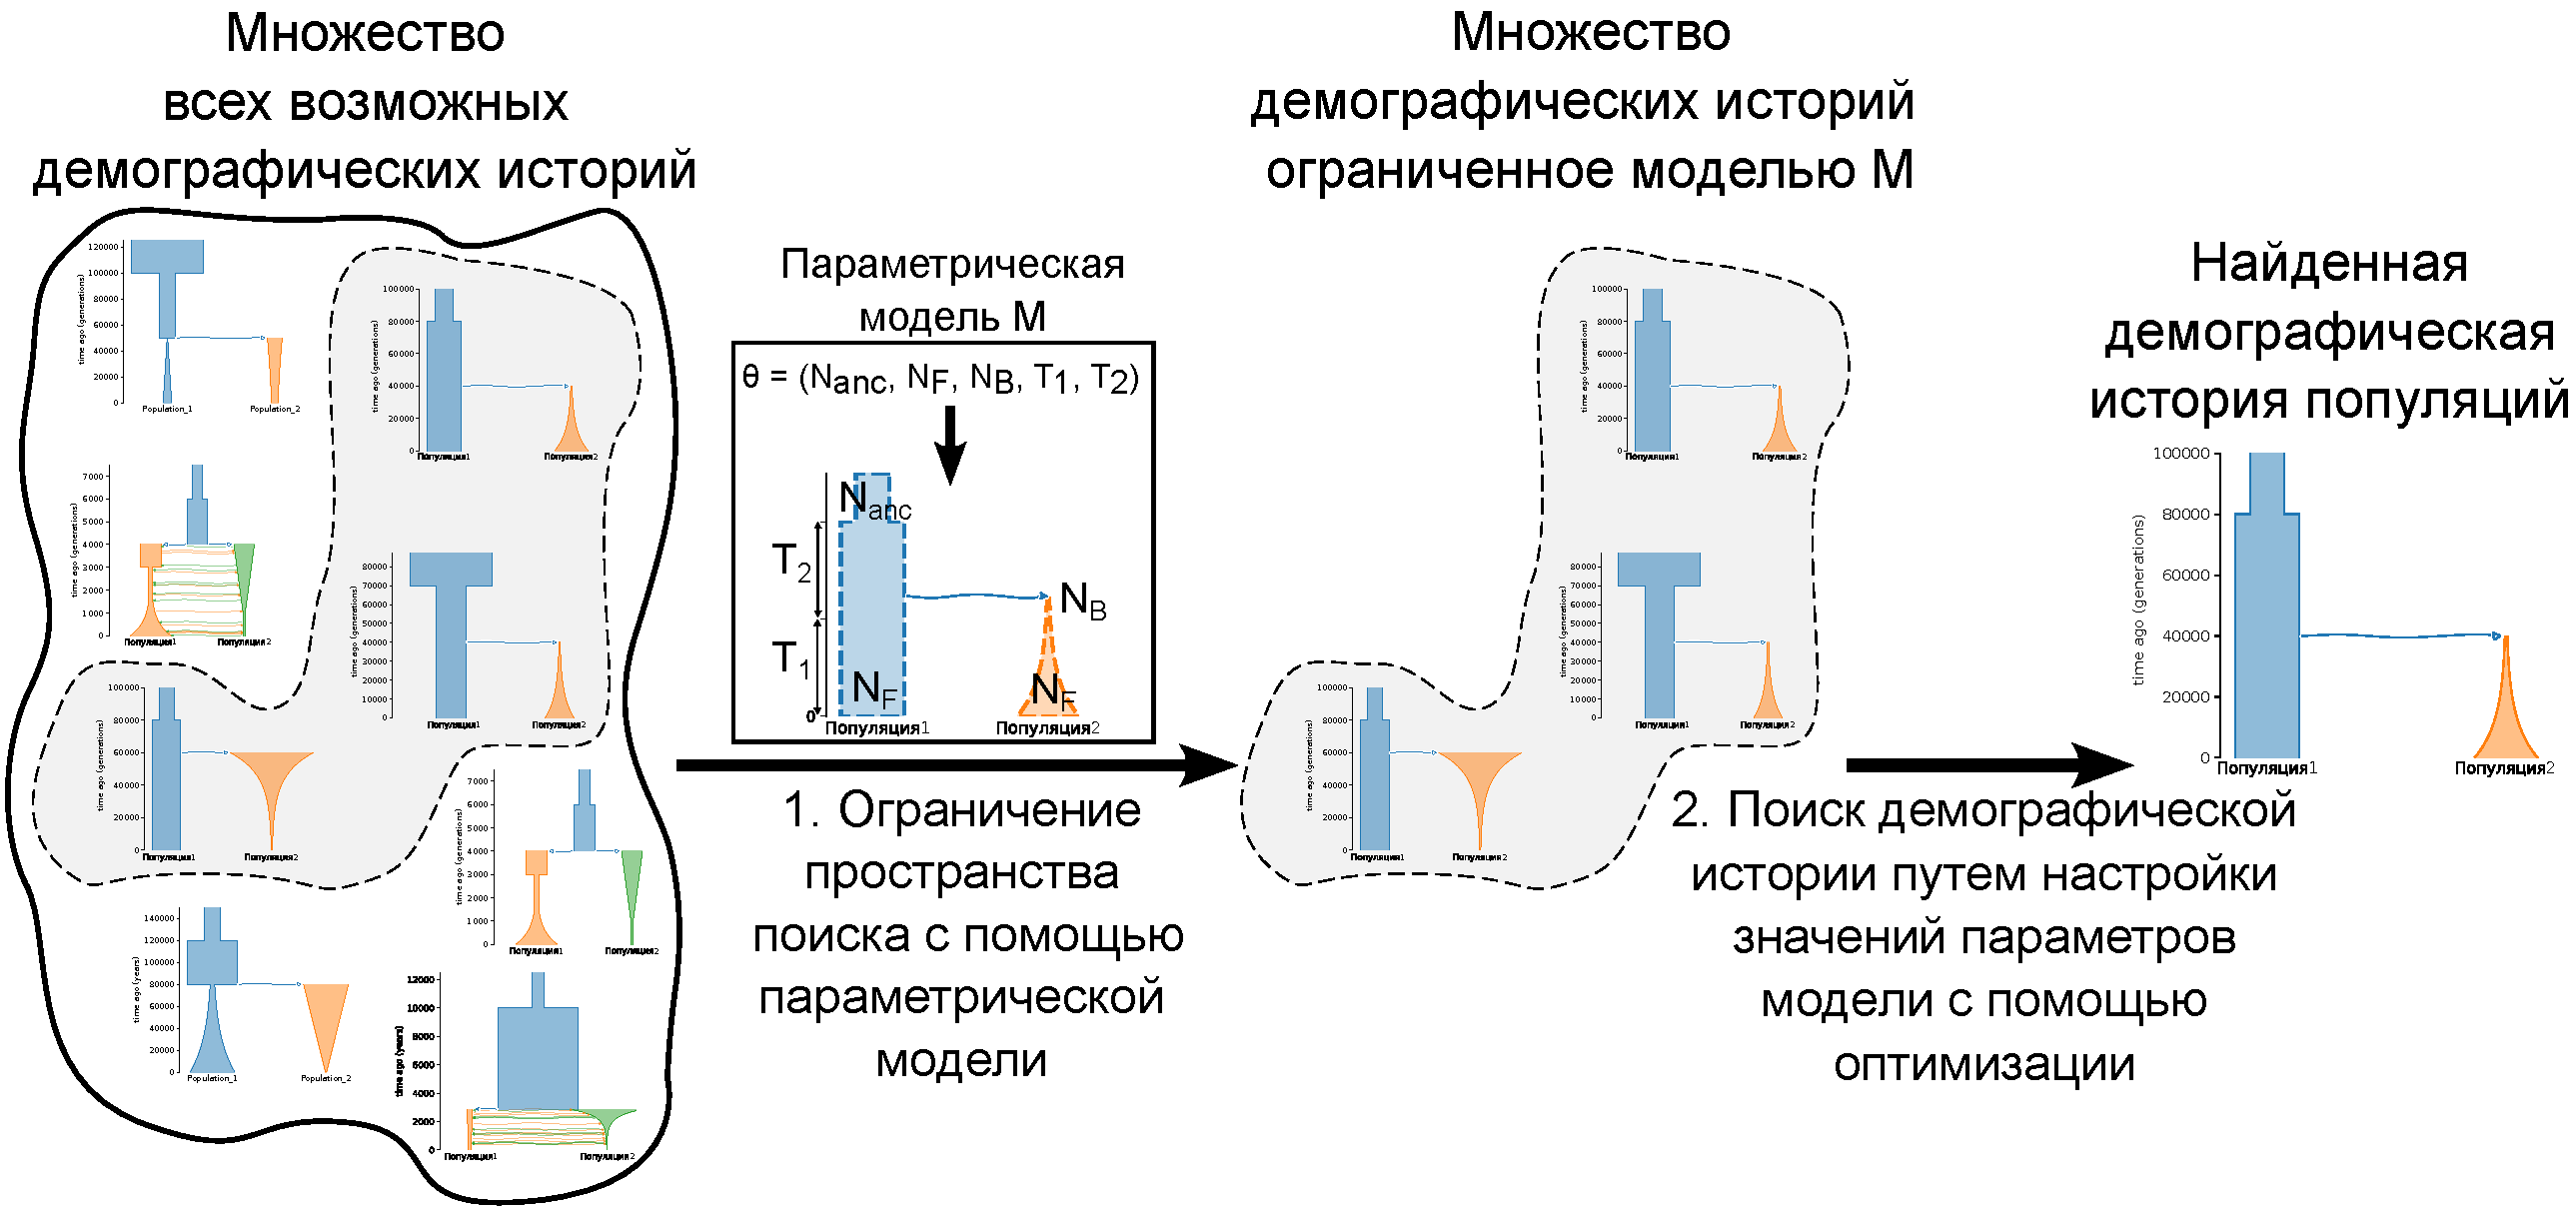
\includegraphics[width=\textwidth]{images_2/scheme.pdf}
    \caption{Общая схема поиска демографической истории популяций с использованием параметрической модели}
    \label{fig:scheme}
\end{figure}

Существует несколько программных решений для поиска демографической истории популяций по генетическим данным. 
Все они требуют задания параметрической модели демографической истории и алгоритма вывода ее параметров.
Заметим, что каждое решение ограничено использованием определенного класса моделей с непрерывными параметрами.
Законы изменения численности популяций в таких моделях всегда фиксированы.

Иногда с целью расширить пространство поиска пользователь может использовать несколько моделей и настраивать их параметры независимо.
Например, можно задать модели, отличающиеся законом изменения численности.

В данной работе в качестве аналогов указаны четыре известных решения: \dadi, \moments, \momentsLD, \momi, которые являются библиотеками для языка программирования Python.
Каждая из этих библиотек имеет собственный интерфейс для задания моделей определенного класса, а также для реализации алгоритма настройки значений параметров.
Однако класс моделей, который используется в \dadi, \moments, \momentsLD, одинаковый, а интерфейсы этих библиотек схожи.

Далее приведем описание библиотек \dadi и \momi, однако все разработанные в работе методы применимы и для библиотек \moments и \momentsLD.
Будут приведены определения используемых классов моделей, указаны их недостатки, а также на примерах будет показано использование интерфейсов этих библиотек.
Затем, для всех четырех библиотек будут приведены существующие методы ручного и автоматического перебора моделей для поиска демографической истории популяций.\\

\textbf{1. Библиотека \dadi\myfootcite{gutenkunst2009inferring} для программной реализации модели демографической истории и алгоритма вывода ее параметров}

Эта библиотека реализует метод аппроксимации диффузии и вычисления функции правдоподобия демографической истории и генетических данных.
Она работает только с первым классом моделей, который будет определен далее.

Вход:
\begin{itemize}
    \item генетические данные; характеристики популяций (скорости мутации);
    \item написанный вручную пользователем биоинформатиком программный код для вывода демографической истории, который включает:
    \begin{itemize}
        \item размер сетки для численных вычислений.
        \item спецификацию модели первого класса с непрерывными параметрами;
        \item начальные значения параметров модели или способ их генерации случайным образом;
        \item выбор метода оптимизации (BFGS, метод Пауэлла, метод Нелдера-Мида или алгоритм BOBYQA).
        \item число перезапусков выбранного алгоритма оптимизации для разных значений начальных параметров.
    \end{itemize}
\end{itemize}

Выход:
\begin{itemize}
    \item демографическая история популяций, как модель с настроенными значениями параметров, которая имеет максимальное значение правдоподобия с генетическими данными.\\
\end{itemize}


%Библиотека \dadi использует модели, которые описываются временными интервалами и раздлениями.
Для определения класса моделей, который используется в библиотеке \dadi, дадим определение элементов модели: временного интервала и разделения.

Временной интервал описывает некий промежуток во времени определенной длины, в течение которого для каждой популяции из набора заданы начальная и конечная численность, а также закон функции изменения численности: константный, линейный, экспоненциальный.
Элемент разделения определяет популяцию, которая разделилась.

Модель первого класса --- это параметрическая модель демографической истории, которая описывается набором временных интервалов и разделений.
Дадим формальные определения.

\definition Элемент временного интервала $\mathcal{I}$ --- это пятерка $<p, T, \mathfrak{N}^{start}, \mathfrak{N}^{end}, \mathfrak{d}>$, где $p \in \mathbb{N}$ --- число популяций, $T$ --- время продолжительности временного интервала, $\mathfrak{N}^{start} = \{N^s_1, \cdots,N^s_p\}$ --- численности каждой из популяций в начале временного интервала, $\mathfrak{N}^{end} = \{N^e_1, \cdots,N^e_p\}$ --- численности каждой из популяций в конце, $\mathfrak{d} = \{d_1, \cdots,d_p\},\ d_i \in \{0, 1, 2\}$ --- закон изменения численности.

\definition Характеристиками $\chi(\mathcal{I})$ временного интервала $\mathcal{I}$ называется множество
$\{T, N^s_1, \cdots,N^s_p, N^e_1, \cdots,N^e_p\}$.

\definition Элемент разделения $\mathcal{S}$ --- это набор из двойка чисел $<p, i>$, где $p$ --- число популяций до разделения, $i \in \{1, \cdots, p\}$ --- индекс разделившейся популяции.
Популяция с индексом $i$ разделяется на две популяции с индексами $i$ и $p+1$.
Элемент разделения не имеет характеристик, то есть $\chi(\mathcal{S}) = \emptyset$.

\definition \textbf{Модель первого класса} для демографической истории $P$ популяций --- параметрическая модель для демографической истории $P$ популяций, которая представляется в виде тройки $<\Theta, \mathcal{E}, \mathfrak{F}>$, где $\Theta \subset \mathbb{R}_+^d$~---~множество значений непрерывных параметров модели, $\mathcal{E} = \{E_i\}_{i=1}^K,\ E_i \in \mathcal{I} \cup \mathcal{S}$~---~последовательность элементов временных интервалов и разделений, $\mathfrak{F}: \Theta \to  \bigcup \chi(E_i)$~---~отображение параметров модели в характеристики элементов.

На рисунке~\ref{fig:model_1_type} приведен пример параметрической модели, которая относится к первому классу моделей.
Эта модель описывает демографические истории двух популяций, у которых размер предковой популяции до разделения равен сумме размеров новообразованных популяций после разделения.
Заметим, что такую модель можно представить в виде последовательности $\{I_1, S_1, I_2\}$, где $I_1$, $I_2$ --- элементы временных интервалов, а $S_1$ --- элемент разделения.
Отображение $\mathfrak{F}$ задает зависимости между параметрами и характеристиками модели.
Оно может быть взаимно однозначным --- каждой характеристике элементов ставить параметр в соответствие.
Однако обычно это не так, и число параметров модели строго меньше числа характеристик всех ее элементов.


\begin{figure}[h]
    \centering
    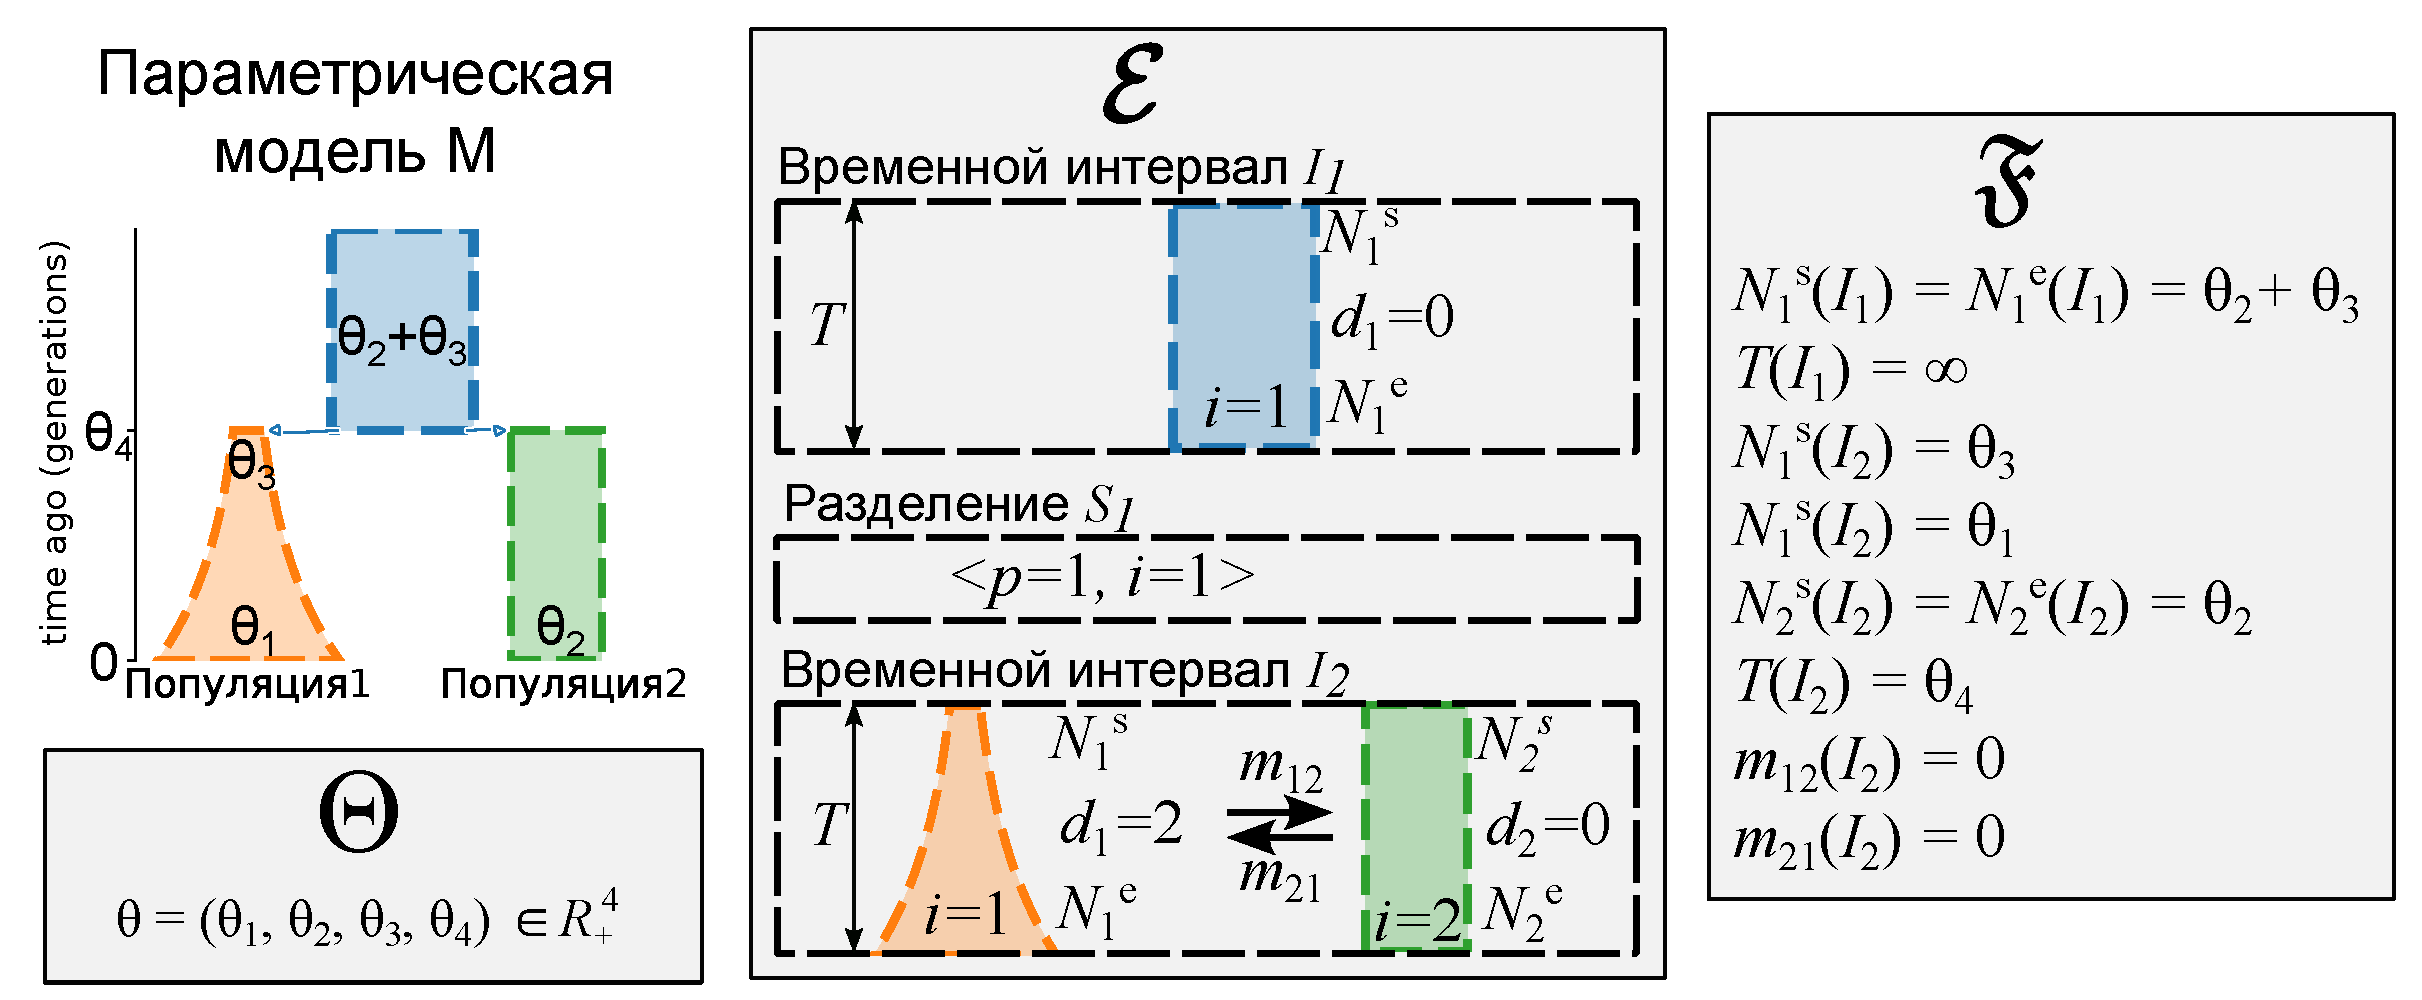
\includegraphics[width=\textwidth]{images_2/model_1_type.pdf}
    \caption{Пример модели $M = <\Theta, \mathcal{E}, \mathfrak{F}>$ первого класса}
    \label{fig:model_1_type}
\end{figure}



\dadi~--- библиотека на языке Python для работы с моделями первого класса.
Она позволяет специфицировать модель первого класса и настроить ее параметры по генетическим данным.
Модель демографической истории реализуется с использованием библиотеки \dadi, как процедура на языке программирования Python.
%Основными элементами программной реализации модели являются временные интервалы и разделения популяций.
%Пример изображения временных интервалов и разделений представлены на рисунке~\ref{fig:dadi:model_spec}.
%Временной интервал определяет изменение численности популяций в модели в течение какого-то заданного промежутка времени в прошлом.
%Разделение задает расщепление одной популяции на две в модели.
%Временной интервал имеет такие параметры, как продолжительность и функциями изменения численности популяций во время интервала.
%Функция изменения численности должна быть задана в явном виде пользователем, но обычно она выбирается из некого стандартного набора функций: константная, линейная или экспоненциальная.

Приведем пример как пользователь может специфицировать модель первого класса с помощью интерфейса \dadi.
Для этого рассмотрим модель демографической истории двух популяций, изображенную на рисунке~\ref{fig:dadi:model}.
%Напомним, что разные цвета закрашенных областей соответствуют разным популяциям, а ширина этих областей в каждый момент времени определяется численностью.
Схематичное изображение модели представлено на рисунке~\ref{fig:dadi:model_1}.
Из определения модели, как параметрического семейства демографических историй, следует, что модель при каких-то значениях параметров является демографической историей.
На рисунке~\ref{fig:dadi:model_2} приведены демографические истории, которые соответствуют модели со следующими значениями параметров:
\begin{enumerate}[label={\arabic*}.]
    \item \texttt{Nanc}: 7200, \texttt{Tp}: 40000, \texttt{N1F}: 13000, \texttt{T}: 40000, \texttt{N2B}: 500, \texttt{N2F}: 12500;
    \item \texttt{Nanc}: 7200, \texttt{Tp}: 80000, \texttt{N1F}: 35000, \texttt{T}: 20000, \texttt{N2B}: 500, \texttt{N2F}: 12500;
    \item \texttt{Nanc}: 7200, \texttt{Tp}: 20000, \texttt{N1F}: 13000, \texttt{T}: 60000, \texttt{N2B}: 30000, \texttt{N2F}: 500;
    \item \texttt{Nanc}: 30000, \texttt{Tp}: 30000, \texttt{N1F}: 13000, \texttt{T}: 40000, \texttt{N2B}: 500, \texttt{N2F}: 12500;
\end{enumerate}

\begin{figure}[h]
    \centering
    \begin{subfigure}[c]{.5\textwidth}
    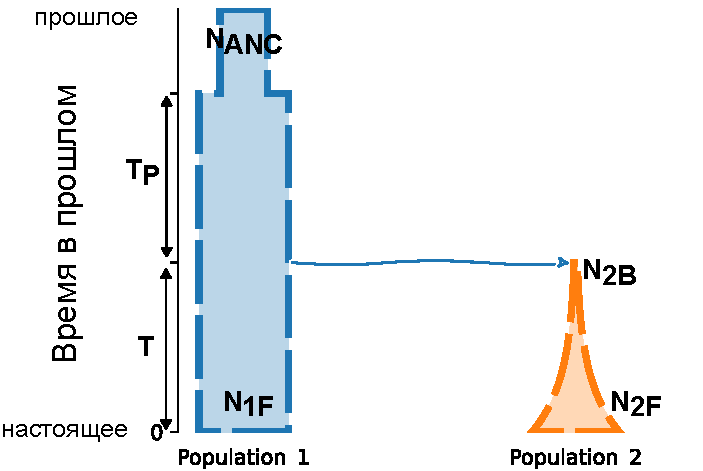
\includegraphics[width=\textwidth]{images_2/picture_2pops_model_1.pdf}
    \caption{}
    \label{fig:dadi:model_1}
    \end{subfigure}%
    \begin{subfigure}[c]{.49\textwidth}
    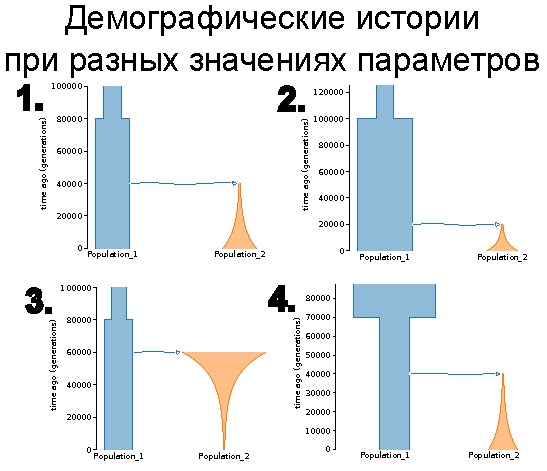
\includegraphics[width=\textwidth]{images_2/picture_2pops_model_1_2.pdf}
    \caption{}
    \label{fig:dadi:model_2}
    \end{subfigure}
    \caption{Модель демографической истории с параметрами и демографические истории при разных значениях параметров}
    \label{fig:dadi:model}
\end{figure}

Данная модель соответствует тому, что давно в прошлом была одна популяция размера \texttt{Nanc} особей, затем она в какой-то момент начала меняться.
Сначала был временной интервал продолжительностью \texttt{Tp} поколений, в течение которого размер популяции был константным и равным \texttt{N1F} особей.
После окончания этого интервала от этой популяции отделилась вторая популяция.
После разделения на протяжении \texttt{T} поколений (второй временной интервал) первая популяция имела ту же константную численность \texttt{N1F} особей, а вторая популяция имела экспоненциальное изменение численности от \texttt{N2B} до \texttt{N2F} особей.
После этого наступил настоящий момент времени, когда существуют обе рассматриваемые популяции.
Все только что описанные параметры \texttt{Nanc}, \texttt{Tp}, \texttt{N1F}, \texttt{T}, \texttt{N2B} и \texttt{N2F} --- это параметры рассматриваемой модели.

Это модель первого класса, так как она представляется в виде последовательности $\{I_1, I_2, S_1, I_3\}$, где $I_1$, $I_2$, $I_3$ --- элементы временных интервалов, а $S_1$ --- элемент разделения.
Эти элементы показаны на рисунке~\ref{fig:dadi:model_spec}.

Теперь рассмотрим как будет выглядеть интерфейс \dadi для задания этой модели.
Для программной реализации модели требуется реализовать процедуру \texttt{model} на языка программирования Python, которая на вход принимает переменные --- параметры модели.
Рисунок~\ref{fig:dadi:model_spec} демонстрирует вид этой функции с использованием \dadi для задания модели.
В теле функции последовательно определяются элементы временных интервалов и зависимость их характеристик от параметров модели: сначала создается первый элемент временного интервала $I_1$ с константной численностью \texttt{Nanc} одной популяции, затем создается второй временной интервал $I_2$ длины $T(I_2) = \text{\texttt{Tp}}$ с константной численностью $N_1^s(I_2) = N_1^e(I_2) = \text{\texttt{N1F}}$ одной популяции, после следует элемент разделения первой популяции на две и, наконец, третий элемент временного интервала длины \texttt{T} для двух популяций, одна из которых имеет константную численность $N_1^s(I_3) = N_1^e(I_3) = \text{\texttt{N1F}}$, а вторая экспоненциальное изменение $d_2(I_3) = 2$ от $N_1^s(I_3) = \text{\texttt{NB}}$ до $N_1^e(I_3) = \text{\texttt{N2F}}$.
\begin{figure}[h]
    \centering
    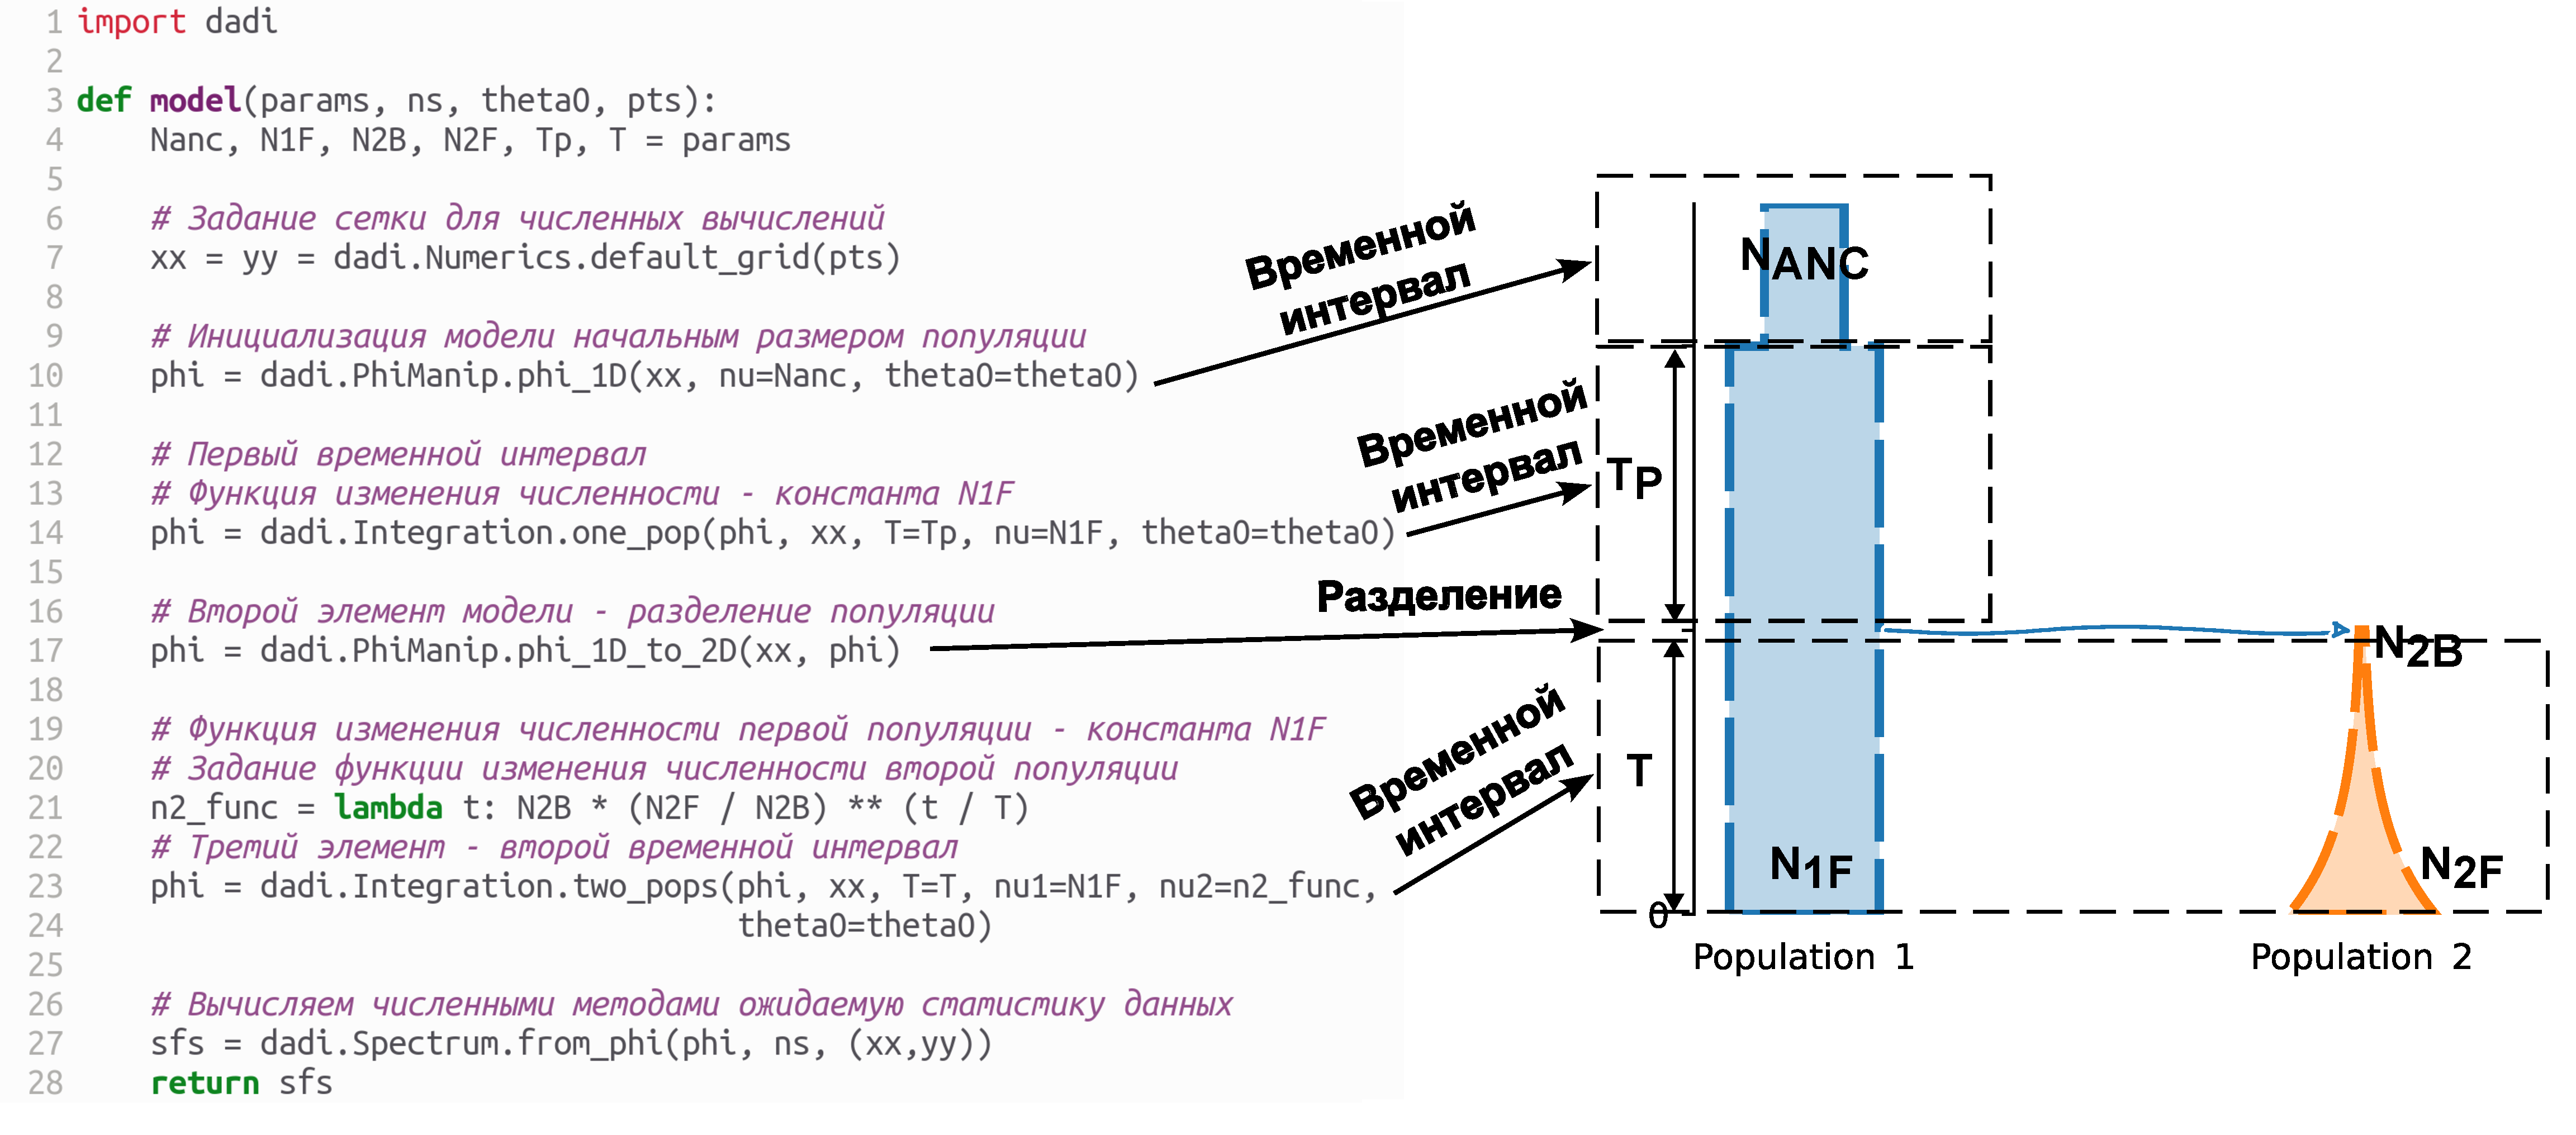
\includegraphics[width=\linewidth]{images_2/dadi_model.pdf}
    \caption{Пример задания модели демографической истории с использованием интерфейса библиотеки~\dadi}
    \label{fig:dadi:model_spec}
\end{figure}

Такой способ задания модели имеет ряд неудобств для пользователя, например, создание сетки \texttt{xx} для численных вычислений с использованием аргумента \texttt{pts}, а также передача \texttt{xx} и объекта \texttt{phi} во все используемые процедуры библиотеки.
Это следствие того, что реализуемая процедура напрямую вычисляет значение ожидаемой статистики данных \texttt{sfs} для специфицированной демографической истории.
Объект \texttt{phi} является решением уравнения диффузии, которое находится с использованием численных методов с сеткой \texttt{xx}.
Модель, заданная описанным образом с помощью библиотеки \dadi, может быть использована исключительно только для \dadi.

Величина \texttt{theta0} равна $4\cdot \mu \cdot L$, где $\mu$ --- это скорость мутации особей рассматриваемого вида, а $L$ --- длина генетической последовательности генетических данных.
Значения $\mu$ и $L$, а следовательно и \texttt{theta0}, определены пользователем.
Множитель «4» присутствует в формуле в силу сложившихся области популяционной генетики обозначений~\myfootcite{gutenkunst2009inferring}.

Для того, чтобы сделать вывод параметров такой модели, требуется запустить оптимизацию, используя строки кода, показанные на рисунке~\ref{fig:dadi:ls_run}.
\begin{figure}[h]
    \centering
    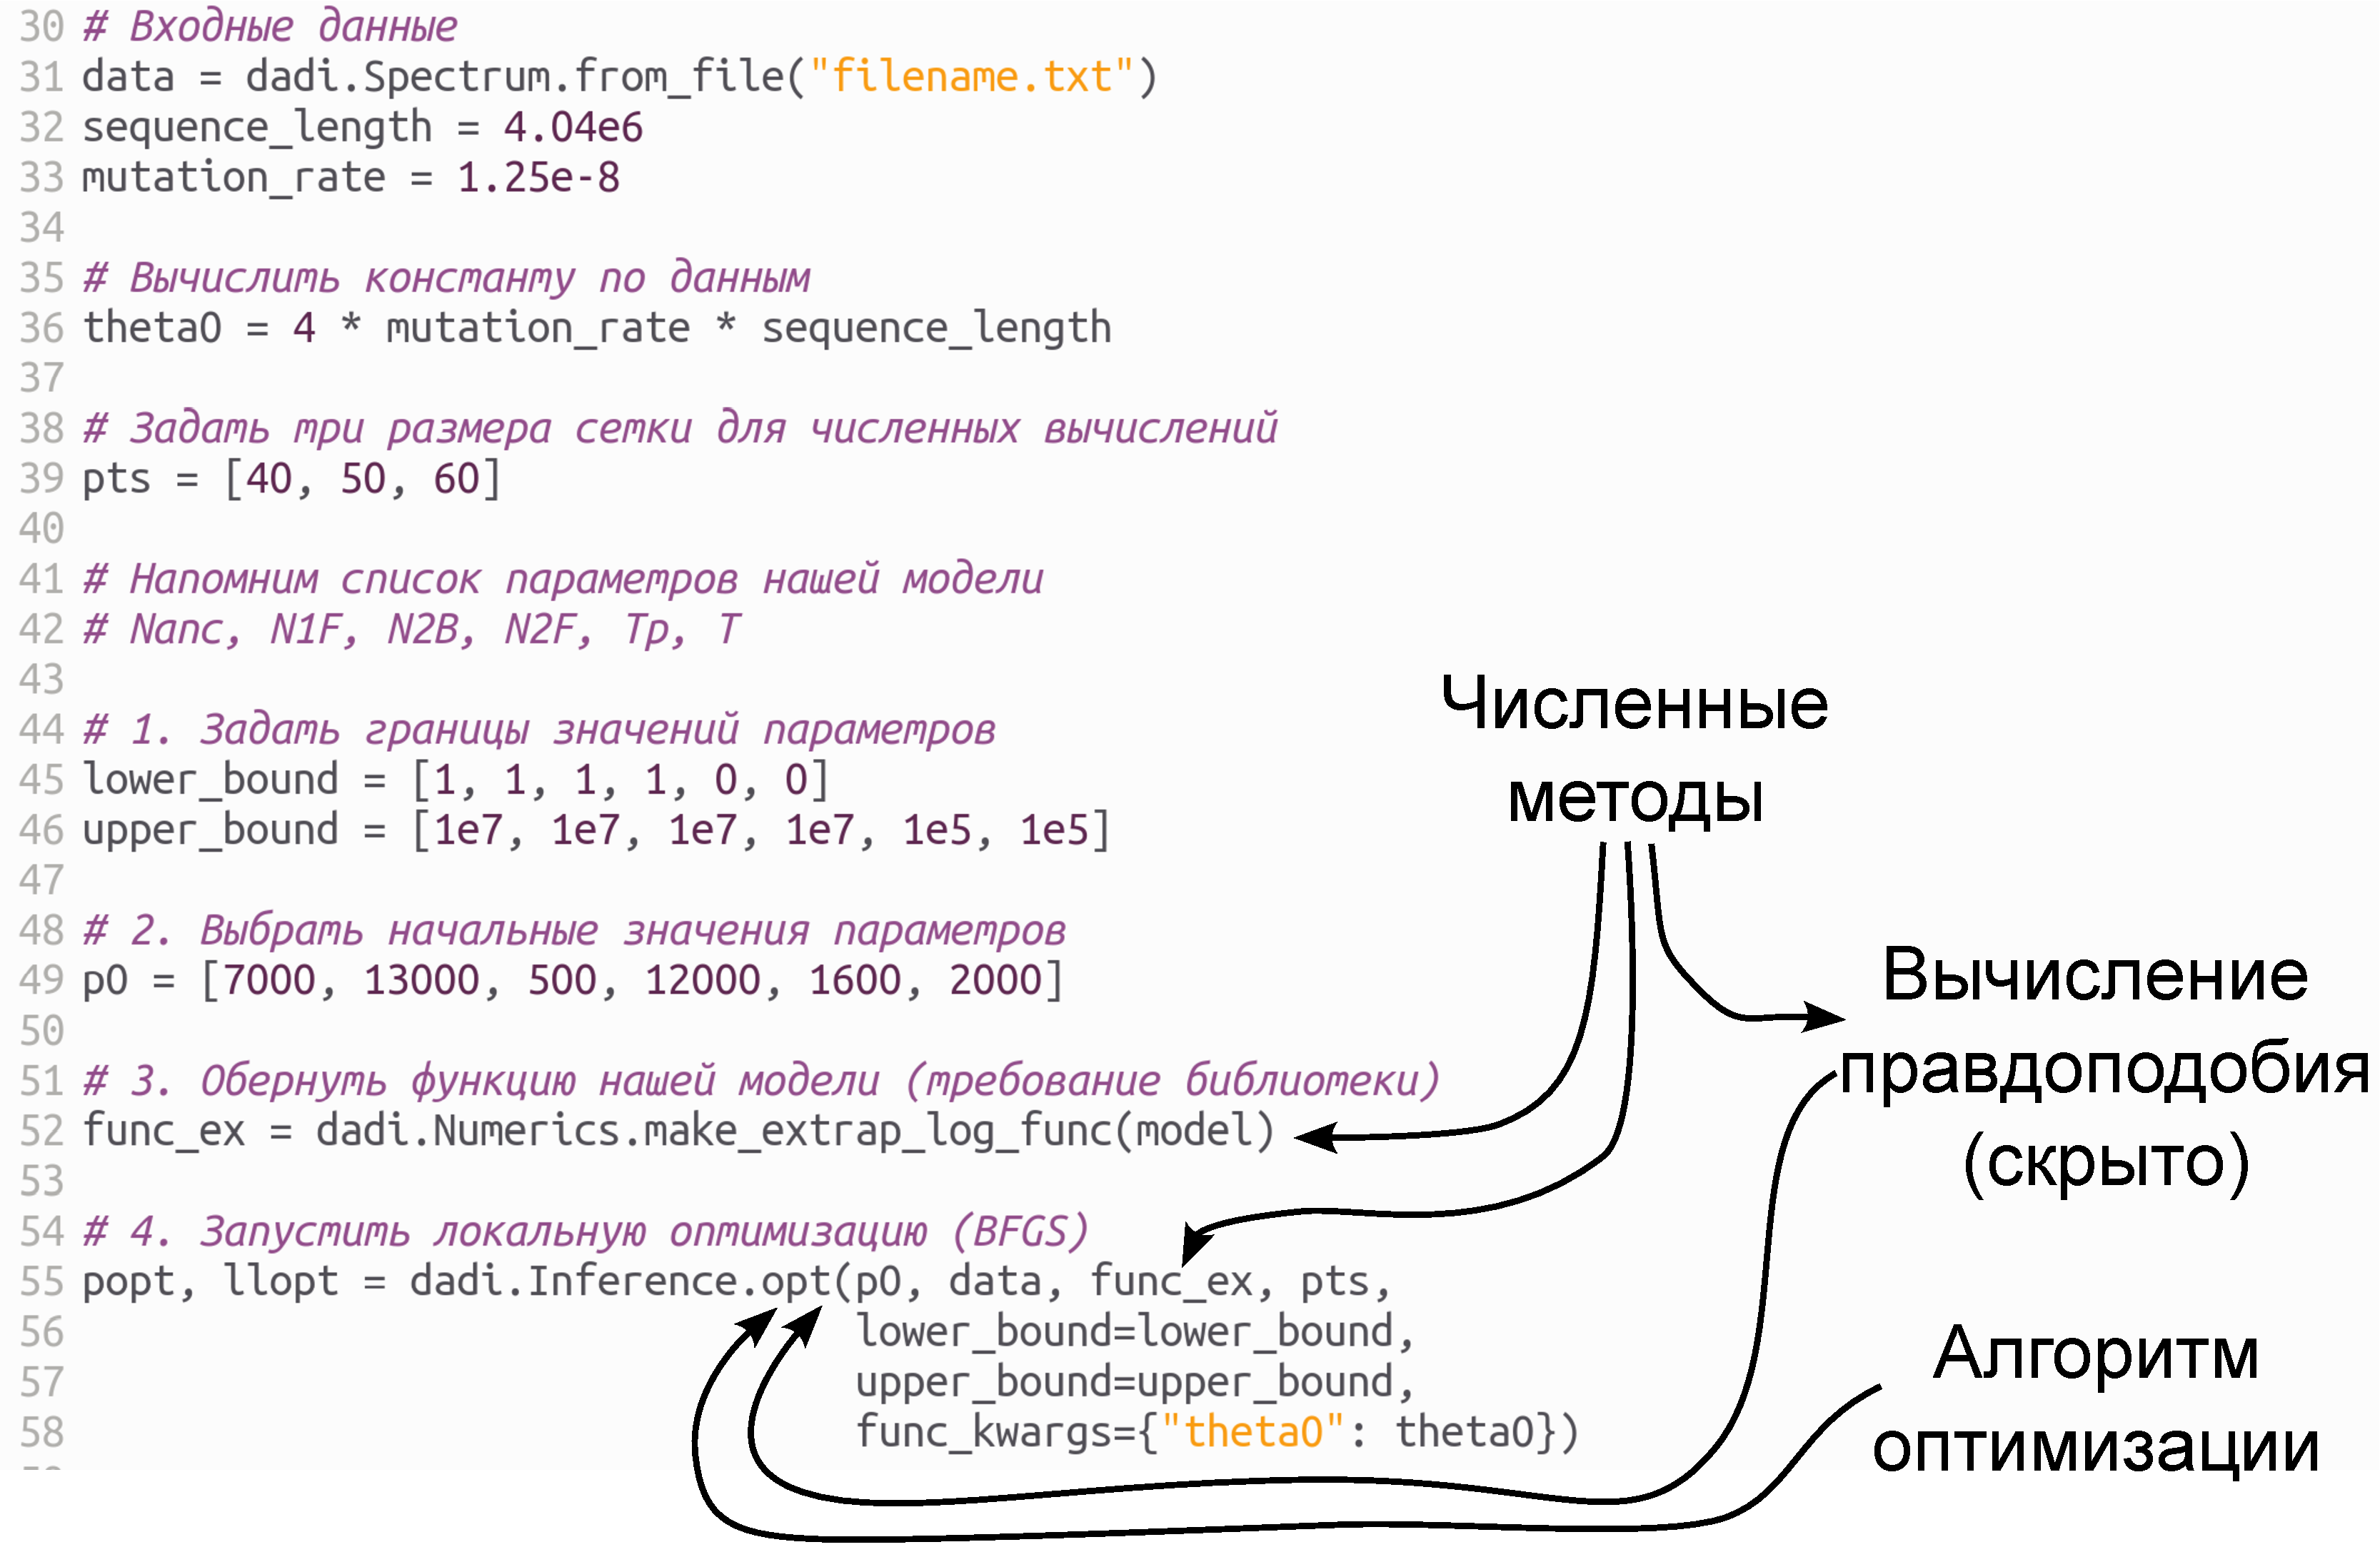
\includegraphics[width=0.8\linewidth]{images_2/dadi_local_search.pdf}
    \caption{Пример реализации алгоритма для поиска параметров модели демографической истории с использованием библиотеки \dadi}
    \label{fig:dadi:ls_run}
\end{figure}

На выходе получаем список \texttt{popt} значений параметров, которые имеют максимальное значение правдоподобия с данными.
Используемый код учитывает особенности библиотеки, например, шаг 3, который требуется для использования численных методов при вычислении ожидаемой статистики данных и правдоподобия.
Для шага 1 существуют рекомендованные значения границ для параметров, однако их все равно необходимо задавать каждый раз вручную.
Поиск параметров модели осуществляется с использованием алгоритма оптимизации на шаге 4.
Библиотека предоставляет несколько алгоритмов оптимизации: BFGS, метод Пауэлла, метод Нелдера-Мида или алгоритм BOBYQA, все они являются методами локальной оптимизации и требуют начальных значений параметра (шаг 2, \texttt{p0}).
В рассматриваемом примере выбрана процедура рекомендованного метода BFGS (\texttt{dadi.Inference.opt}).
Внутри данная процедура выполняет запуск алгоритма оптимизации, а в качестве целевой функции использует значение правдоподобия генетических данных при заданных параметрах модели.
При этом вычисление самого правдоподобия зашито внутри используемой процедуры оптимизации.
Чтобы вычислить правдоподобие для параметров \texttt{p} как внутри процедуры, так и снаружи, можно задать процедуру \texttt{f\_ll}, показанную на рисунке~\ref{fig:dadi:ll_func}.
\begin{figure}[h]
    \centering
    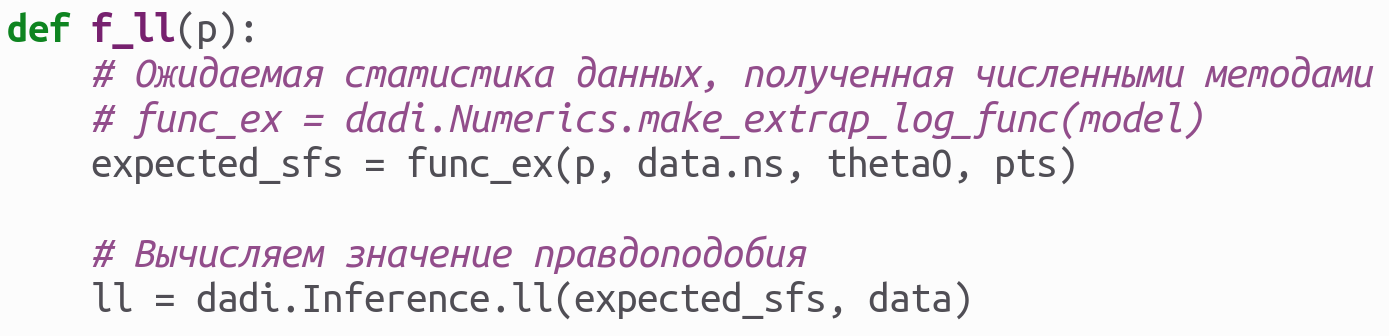
\includegraphics[width=0.6\linewidth]{images_2/dadi_ll.png}
    \caption{Пример реализации функции вычисления правдоподобия для библиотеки \dadi}
    \label{fig:dadi:ll_func}
\end{figure}

Алгоритмы локальной оптимизации очень сильно ограничены заданными начальными значениями параметров.
Эти методы ищут локальный оптимум --- точку, которая находится недалеко от представленной начальной точки и в которой значение правдоподобия максимально в некой окрестности.
Однако нас интересует глобальный оптимум --- значения параметров, которые имеют максимальное значение правдоподобия среди всех возможных точек.
Для того, чтобы найти его с помощью локальных оптимизаций, их нужно запускать несколько раз из разных начальных точек.
Это именно то, что рекомендуют делать авторы \dadi, однако библиотека не предоставляет процедуры для множественного запуска локальной оптимизации.
Поэтому каждому пользователю приходится реализовывать это вручную, например, как показано на рисунке~\ref{fig:dadi:ls_run_several}.
\begin{figure}[h]
    \centering
    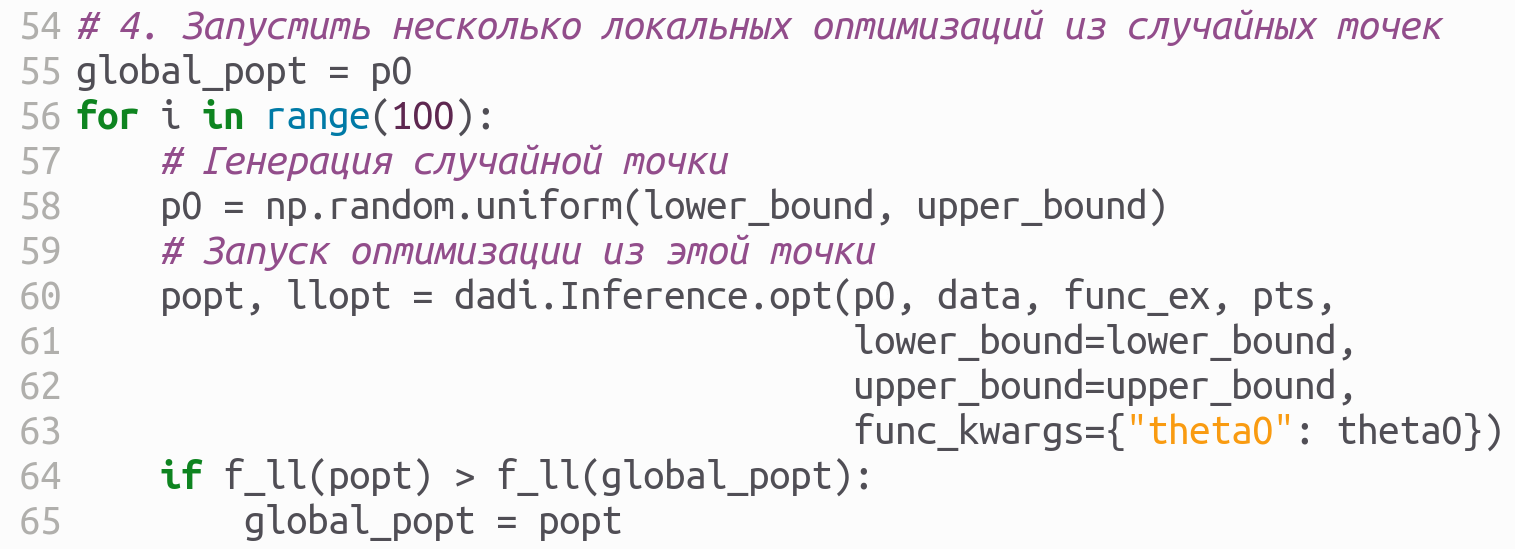
\includegraphics[width=0.6\linewidth]{images_2/dadi_ls_multi.png}
    \caption{Пример реализации алгоритма множественного запуска локальной оптимизации для поиска параметров модели с использованием библиотеки \dadi}
    \label{fig:dadi:ls_run_several}
\end{figure}

\textbf{Выводы по обзору библиотеки \dadi}

Недостатки моделей первого класса:
\begin{itemize}
    \item имеют только непрерывные параметры;
    \item динамики изменения численности (константная численность, линейное или экспоненциальное изменение) фиксированы в моделях.\\
\end{itemize}

Недостатки использования библиотеки \dadi для спецификации моделей:
\begin{itemize}
    \item позволяет работать только с моделями первого класса;
    \item каждая модель специфицируется вручную с использованием специфичного интерфейса библиотеки \dadi;
    \item модели нельзя переиспользовать. Модель, заданную с помощью библиотеки \dadi, можно использовать только для вывода демографической истории с использованием \dadi.
%    \item Динамики изменения численности (константная численность, линейное или экспоненциальное изменение) зафиксированы в моделях.
\end{itemize}

Недостатки использования библиотеки \dadi для настройки значений параметров модели демографической истории:
\begin{itemize}
    \item пользователю требуется задавать и проверять каждую модель вручную с использованием библиотеки \dadi;
    \item библиотека ограничена выводом значений только для непрерывных параметров;
    \item использование алгоритмов локальной оптимизации не гарантирует нахождение глобального оптимума.\\
\end{itemize}

% Таким образом для вывода демографической истории данных в \dadi нужно предоставить на вход:
% \begin{itemize}
%     \item Генетические данные (\texttt{data}),
%     \item Длина (\texttt{sequence\_length}) предоставленной последовательности,
%     \item Скорость мутации (\texttt{mutation\_rate}) --- вероятность мутации на одной позиции в геноме за одно поколение,
%     \item Размер сетки (\texttt{pts}) для численных вычислений,
%     \item Модель (\texttt{model(...)}) демографической истории, заданная в виде функции, принимающей значения параметров-переменных и возвращающей вычисленную ожидаемую статистику данных,
%     \item Нижние и верхние границы (\texttt{lower\_bound}, \texttt{upper\_bound}) значений параметров модели,
%     \item Начальные значения параметров (\texttt{p0}) модели или способ их генерации случайным образом,
%     \item Выбранный метод оптимизации (BFGS, метод Пауэлла, метод Нелдера-Мида или алгоритм BOBYQA).
%     \item Число перезапусков выбранного алгоритма оптимизации для разных значений начальных параметров,
%     \item Реализация всего вывода в виде программного кода с использованием элементов специфичных для библиотеки \dadi.
% \end{itemize}
% На выход исследователь получает:
% \begin{itemize}
%     \item Значения параметров, которые получили максимальное значение правдоподобия во время множественных запусков оптимизации.\\
% \end{itemize}

% \textbf{2. Библиотека \moments~\myfootcite{jouganous2017inferring} и ее подмодуль \momentsLD~\myfootcite{ragsdale2019models}\myfootcite{ragsdale2020unbiased} для программной реализации модели демографической истории и алгоритма вывода ее параметров.}

% Библиотека \moments была основана на \dadi.
% Эта библиотека реализует метод моментов для математического моделирования и вычисления функции правдоподобия демографической истории и генетических данных.
% Она является библиотекой для языка программирования Python.
% Основной модуль \moments включает подмодуль \momentsLD, который реализует альтернативный метод численного моделирования.
% Интерфейсы \moments и \momentsLD схожи, поэтому мы опишем его только для библиотеки \moments.

% Вход:
% \begin{itemize}
%     \item Генетические данные; характеристики популяций (скорости мутации).
%     \item Написанный вручную исследователем-биоинформатиком программный код для вывода демографической истории, который включает:
%     \begin{itemize}
%         \item Задание модели демографической истории с непрерывными параметрами; нижние и верхние границы значений параметров.
%         \item Начальные значения параметров модели или способ их генерации случайным образом.
%         \item Выбор метода оптимизации (BFGS, метод Пауэлла, метод Нелдера-Мида).
%         \item Число перезапусков выбранного алгоритма оптимизации для разных значений начальных параметров.
%     \end{itemize}
% \end{itemize}

% Выход:
% \begin{itemize}
%     \item Значения параметров модели, которые получили максимальное значение правдоподобия во время множественных запусков оптимизации.\\
% \end{itemize}


% Недостатки использования библиотеки \moments и ее подмодуля \momentsLD для задания модели демографической истории:
% \begin{itemize}
%     \item Модель задается вручную с использованием специфичного интерфейса библиотеки \moments.
%     \item Модель нельзя переиспользовать. Модель, заданную с помощью библиотеки \moments, можно использовать только для вывода демографической истории с использованием \moments.
%     \item Динамики изменения численности (константная численность, линейное или экспоненциальное изменение) зафиксированы в модели.
% \end{itemize}

% Недостатки использования библиотеки \moments и ее подмодуля \momentsLD для вывода демографической истории:
% \begin{itemize}
%     \item Исследователю требуется задавать и проверять каждую модель вручную с использованием библиотеки \moments.
%     \item Библиотека ограничена выводом значений только для непрерывных параметров.
%     \item Использование алгоритмов локальной оптимизации не гарантирует нахождение глобального оптимума.\\
% \end{itemize}

% Отличия библиотеки \moments от \dadi:
% \begin{itemize}
%     \item Отсутствует необходимость задавать размеры сетки \texttt{pts}, в \moments есть протестированные значения по умолчанию.
%     \item При задании модели с помощью \moments используется другой набор более универсальных процедур. Например, для спецификации временного интервала всегда используется процедура \texttt{integrate}, а в \dadi для этого есть целых три процедуры \texttt{one\_pop}, \texttt{two\_pops} и \texttt{three\_pops} для разных чисел популяций.\\
% \end{itemize}

% Библиотека \moments имеет схожий с \dadi интерфейс для задания модели демографической истории через временные интервалы и разделения популяций.
% Он немного более универсальный и содержит меньшее число узкоспециализированных процедур.
% Например, процедура для разделения популяций в \moments едина, в то время как в \dadi их три и они отличаются индексом разделяемой популяции и общим числом популяций в данный момент времени: 1) разделение единственной популяции, 2) разделение первой популяции в случае двух популяций, 3) разделение второй популяции в случае двух популяций.
% Как и в случае \dadi, модель записывается в виде функции для языка программирования Python, принимающей на вход значения параметров и возвращающей вычисленную ожидаемую статистику данных.
% Пример задания модели, изображенной на рисунке~\ref{fig:dadi:model}, с использованием библиотеки \moments показан на рисунке~\ref{fig:moments:model_spec}.
% \begin{figure}[h]
%     \centering
%     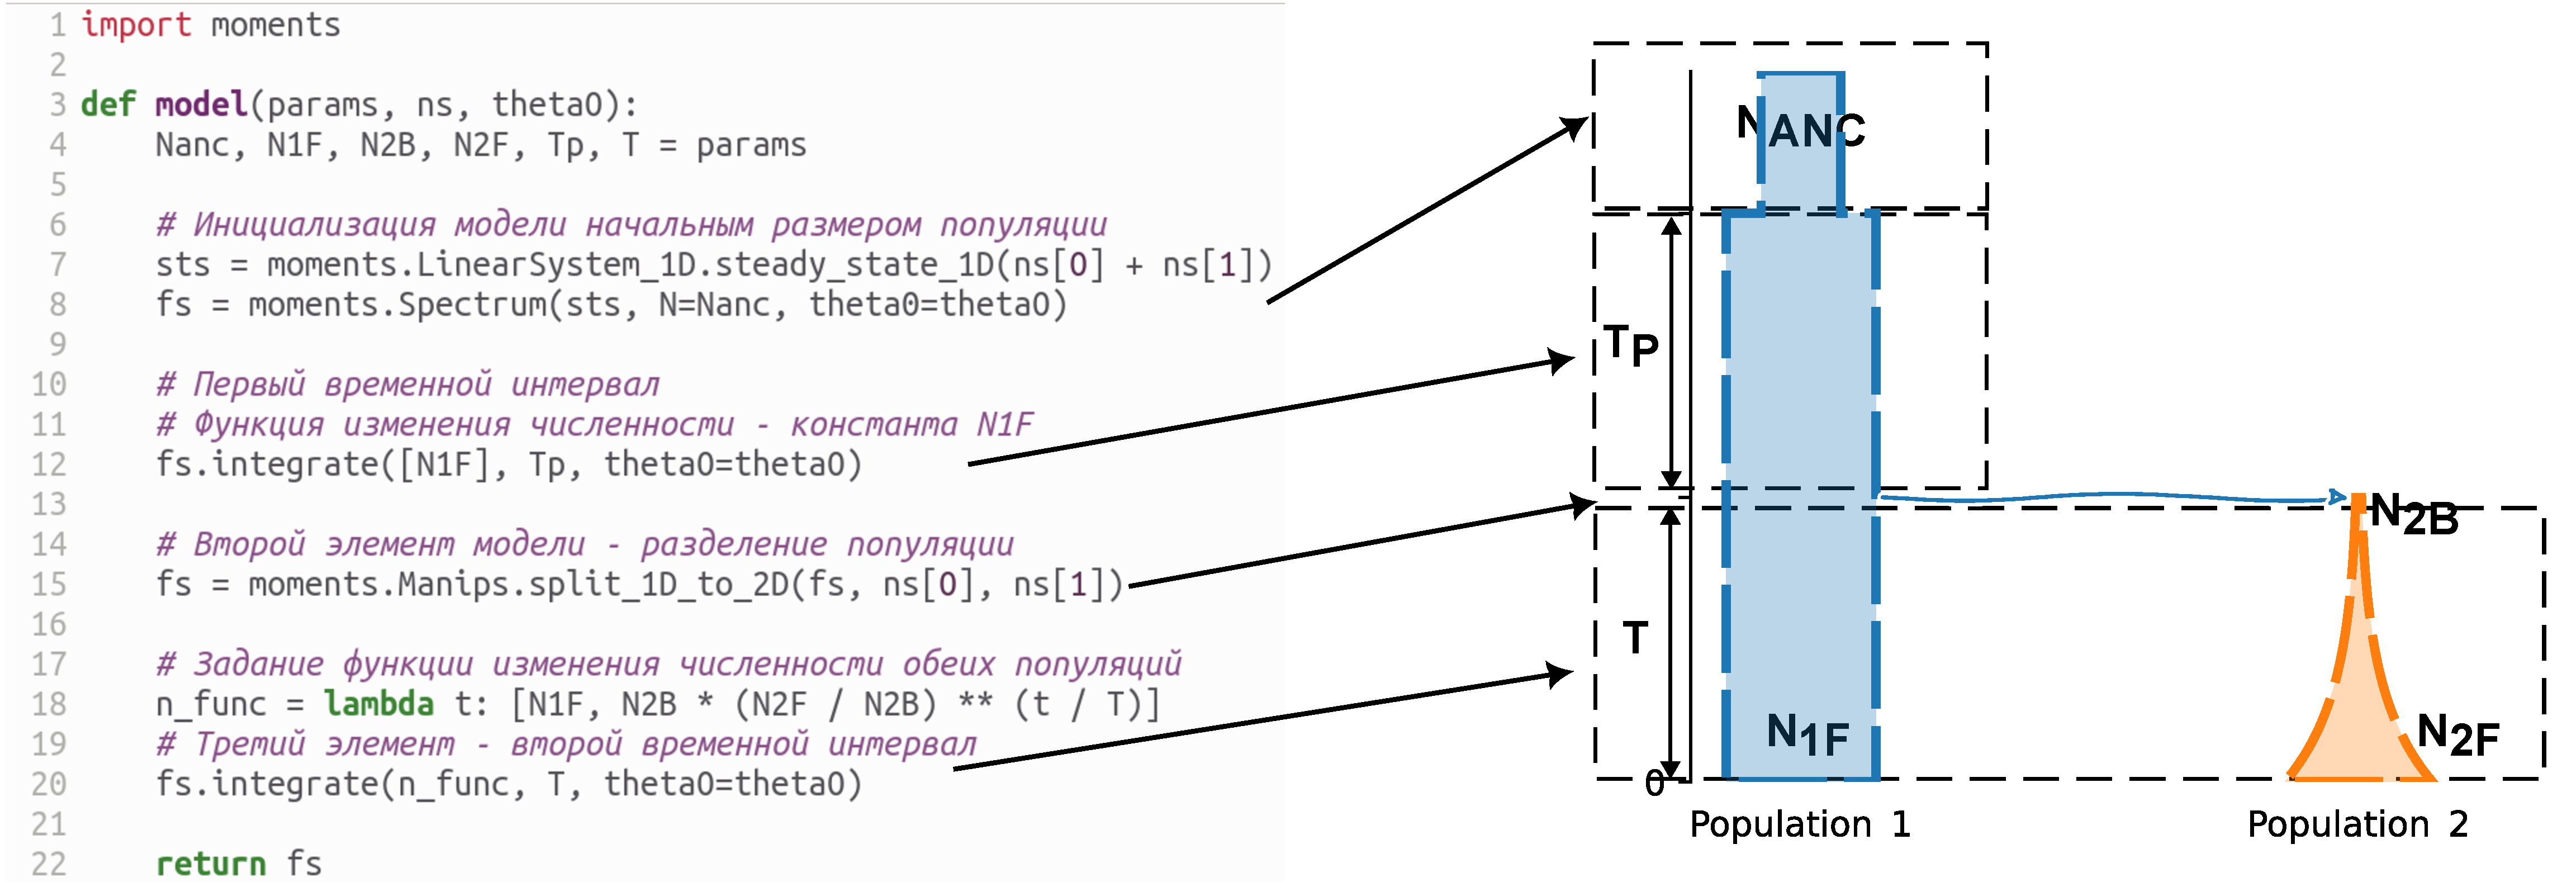
\includegraphics[width=\linewidth]{images_2/moments_model.pdf}
%     \caption{Пример задания модели демографической истории с использованием интерфейса библиотеки~\moments}
%     \label{fig:moments:model_spec}
% \end{figure}

% Интерфейс для реализации алгоритма вывода параметров заданной модели в \moments такой же, как и в \dadi.
% Поэтому программный код, который представлен на рисунке~\ref{fig:dadi:ls_run_several} при замене библиотеки \dadi на \moments будет работать для множественного запуска локальных оптимизаций и поиска параметров с максимальным значением правдоподобия с использованием \moments.\\


\textbf{2. Библиотека \momi~\myfootcite{kamm2020efficiently} для программной реализации модели демографической истории и алгоритма вывода ее параметров}

Эта библиотека реализует метод непрерывной модели Морана для вычисления функции правдоподобия демографической истории и генетических данных.
Она работает только со вторым классом моделей, который будет определен ниже.

Вход:
\begin{itemize}
    \item генетические данные; характеристики популяций (скорости мутации);
    \item написанный вручную пользователем-биоинформатиком программный код для вывода демографической истории, который включает:
    \begin{itemize}
        \item спецификацию модели второго класса с непрерывными параметрами;
        \item начальные значения параметров модели или способ их генерации случайным образом;
        \item число перезапусков алгоритма оптимизации (TNC) для разных значений начальных параметров.
    \end{itemize}
\end{itemize}

Выход:
\begin{itemize}
    \item демографическая история популяций, как модель с настроенными значениями параметров, которая имеет максимальное значение правдоподобия с генетическими данными.\\
\end{itemize}

Библиотека \momi работает с другим классом моделей демографической истории, чем \dadi.
Модель второго класса --- это параметрическая модель демографической истории, которая представляется в виде набора событий изменения численности и разделений.
Событие изменения численности задает численность популяции в какой-то момент времени в прошлом, а также описывает ее изменение до этого момента используя экспоненциальный закон.
Константная численность воспринимается как экспоненциальное изменение со степенью, равной нулю.
События разделений описывают отделение одной популяции от другой, они маркируют вершины дерева разделений модели индексами текущих популяций так, что индекс вершины-родителя всегда равен индексу строго одного из его потомков.

%Событие разделения популяции обязано соответсвовать деревом разделения модели, однако 
%Для ясности дадим строгие определения.

\definition Событие изменения численности $C$ --- это четверка $<p, T, N, r>$, где $p$ --- индекс популяции, численность которой изменилась, $T$ --- время окончания изменения численности, $N$ --- численность популяции в конце, $r$ --- степень экспоненциального изменения популяции.

\definition Характеристиками $\chi(C)$ события изменения численности $C$ называется множество $\{T, N, r\}$.

\definition Событие разделения $U$ --- это двойка $<p_{from}, p_{to}>$, где $p_{from}$ --- индекс популяции, от которой произошло отделение, $p_{to}$ --- индекс популяции, которая образовалась.
Событие разеделения не имеет характеристик, то есть $\chi(U) = \emptyset$.

\definition
\textbf{Модель второго класса} для демографической истории $P$ популяций --- параметрическая модель для демографической истории $P$ популяций, которая представляется в виде тройки $<\Theta, \mathcal{E}, \mathfrak{F}>$, где $\Theta \subset \mathbb{R}_+^d$ --- множество значений непрерывных параметров модели, $\mathcal{E} = \{E_i\}_{i=1}^K,\ E_i \in C \cup U$ --- набор событий изменения численности и разделений, $\mathfrak{F}: \Theta \to \bigcup_i \chi(E_i)$ --- отображение параметров модели в характеристики событий.

Приведем пример модели второго класса.
Модель первого класса, изображенная на рисунке~\ref{fig:model_1_type}, является также и моделью второго класса.
Рисунок~\ref{fig:model_2_type} изображает ее представление, как модели второго класса.

\begin{figure}[h]
    \centering
    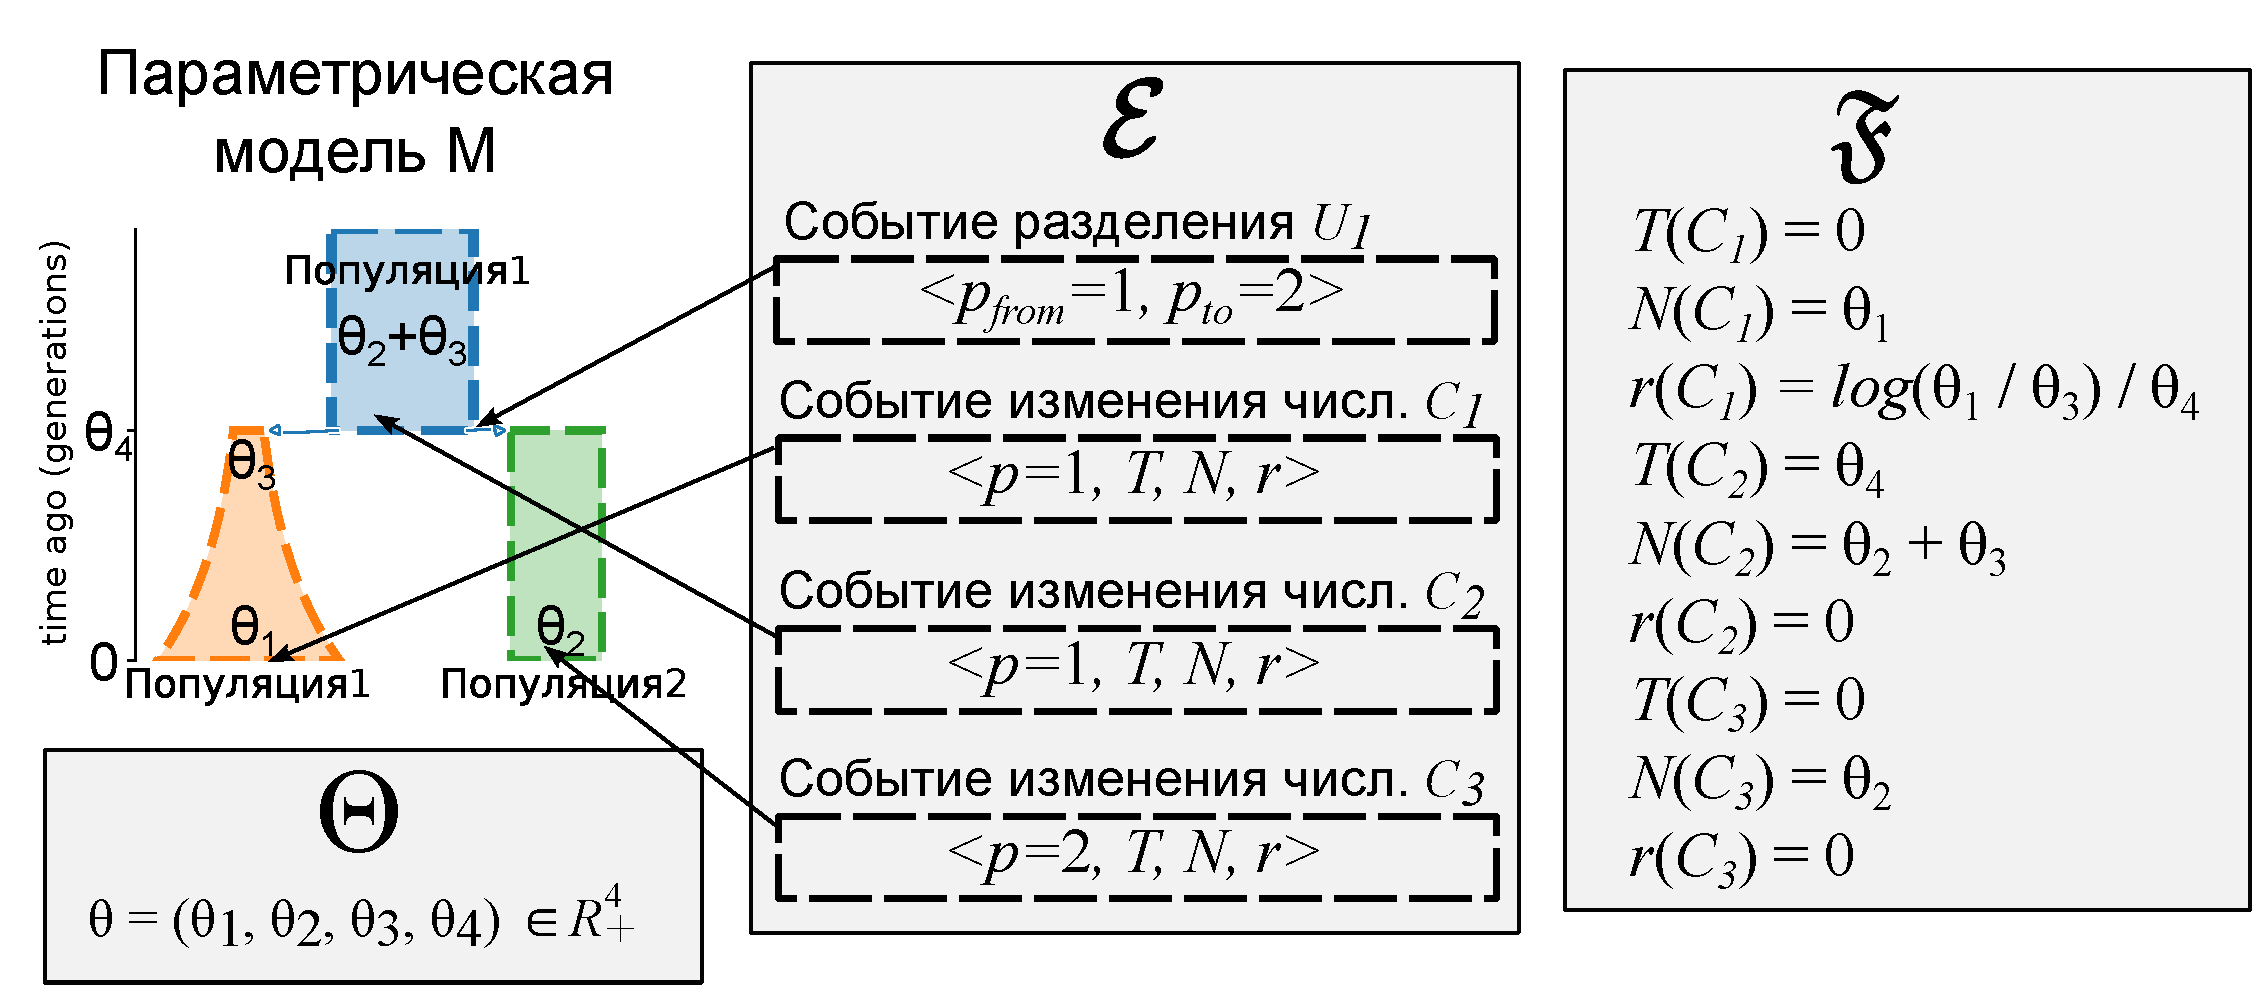
\includegraphics[width=\textwidth]{images_2/model_2_type.pdf}
    \caption{Пример модели $M = <\Theta, \mathcal{E}, \mathfrak{F}>$ второго класса}
    \label{fig:model_2_type}
\end{figure}


Однако первый и второй классы моделей различны.
Приведем пример модели, которая является моделью второго класса и не относится к моделям первого класса.
Опишем ее следующим образом.

Рассмотрим две популяции.
Первая из них существовала с момента существования вида ($\infty$ поколений назад) и ее начальная численность была \texttt{Nanc} особей.
Эта первая популяция в какой-то момент времени \texttt{Tc} поколений назад изменила свою численность, и размер популяции стал равен \texttt{N1F} особей.
Вторая популяция отделилась от первой \texttt{T} поколений назад и имела экспоненциальный рост численности со степенью \texttt{r2} и ее численность в настоящий момент составляет \texttt{N2F} особей.
Все только что описанные параметры \texttt{Nanc}, \texttt{Tc}, \texttt{N1F}, \texttt{T}, \texttt{r2} и \texttt{N2F} --- это параметры рассматриваемой модели.

Изображение этой модели представлено на рисунке~\ref{fig:momi:model_1}.
На рисунке~\ref{fig:momi:model_2} приведены демографические истории, которые соответствуют модели со следующими значениями параметров:
\begin{enumerate}[label={\arabic*}.]
    \item \texttt{Nanc}: 7200, \texttt{Tc}: 80000, \texttt{N1F}: 13000, \texttt{T}: 40000, \texttt{r2}: $8\cdot 10^{-5}$, \texttt{N2F}: 12500;
    \item \texttt{Nanc}: 7200, \texttt{Tc}: 100000, \texttt{N1F}: 35000, \texttt{T}: 20000, \texttt{r2}: $16\cdot 10^{-5}$, \texttt{N2F}: 12500;
    \item \texttt{Nanc}: 7200, \texttt{Tc}: 30000, \texttt{N1F}: 13000, \texttt{T}: 60000, \texttt{r2}: $5\cdot 10^{-5}$, \texttt{N2F}: 12500;
    \item \texttt{Nanc}: 30000, \texttt{Tc}: 30000, \texttt{N1F}: 13000, \texttt{T}: 60000, \texttt{r2}: $-1\cdot 10^{-5}$, \texttt{N2F}: 10000;
\end{enumerate}

\begin{figure}[h]
    \centering
    \begin{subfigure}[c]{.5\textwidth}
    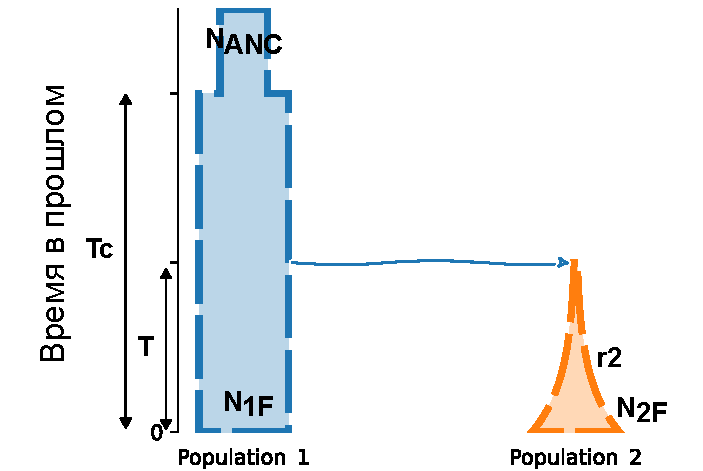
\includegraphics[width=\textwidth]{images_2/picture_2pops_model_2_1.pdf}
    \caption{}
    \label{fig:momi:model_1}
    \end{subfigure}%
    \begin{subfigure}[c]{.49\textwidth}
    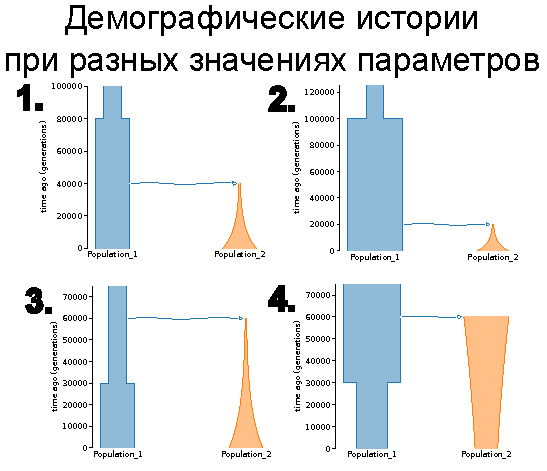
\includegraphics[width=\textwidth]{images_2/picture_2pops_model_2_2.pdf}
    \caption{}
    \label{fig:momi:model_2}
    \end{subfigure}
    \caption{Модель демографической истории с параметрами и демографические истории при разных значениях параметров}
    \label{fig:momi:model}
\end{figure}

Параметры общие для моделей, изображенных на рисунках~\ref{fig:dadi:model_1} и ~\ref{fig:momi:model_1}, имеют одинаковые названия.
Однако модель на рисунке~\ref{fig:momi:model_1} имеет два новых параметра: \texttt{r2} и \texttt{Tc}.
Заметим, что если значение параметра \texttt{Tc} больше, чем значение параметра \texttt{T}, то эту модель можно легко перевести в модель, показанную на рисунке~\ref{fig:dadi:model_1}, используя следующие уравнения для значений параметров \texttt{Tp} и \texttt{N2B}:
$$\text{\texttt{Tp}} = \text{\texttt{Tc}} - \text{\texttt{T}}$$ 
$$\text{\texttt{N2B}} = \text{\texttt{N2F}} \cdot e^{-\text{\texttt{r2}}\cdot \text{\texttt{T}}}.$$

При реализации модели с использованием библиотеки \momi пользователю требуется задать объект специального класса \texttt{momi.DemographicModel}.
Это способствует переиспользованию этого класса для других программных средств.
Для задания модели требуется спецификация объектов параметров-переменных, для каждого из которых можно указать границы, однако, библиотека предоставляет значения границ по умолчанию.
Рисунок~\ref{fig:momi:model_spec} показывает реализацию модели с использованием библиотеки \momi.
\begin{figure}[h!]
    \centering
    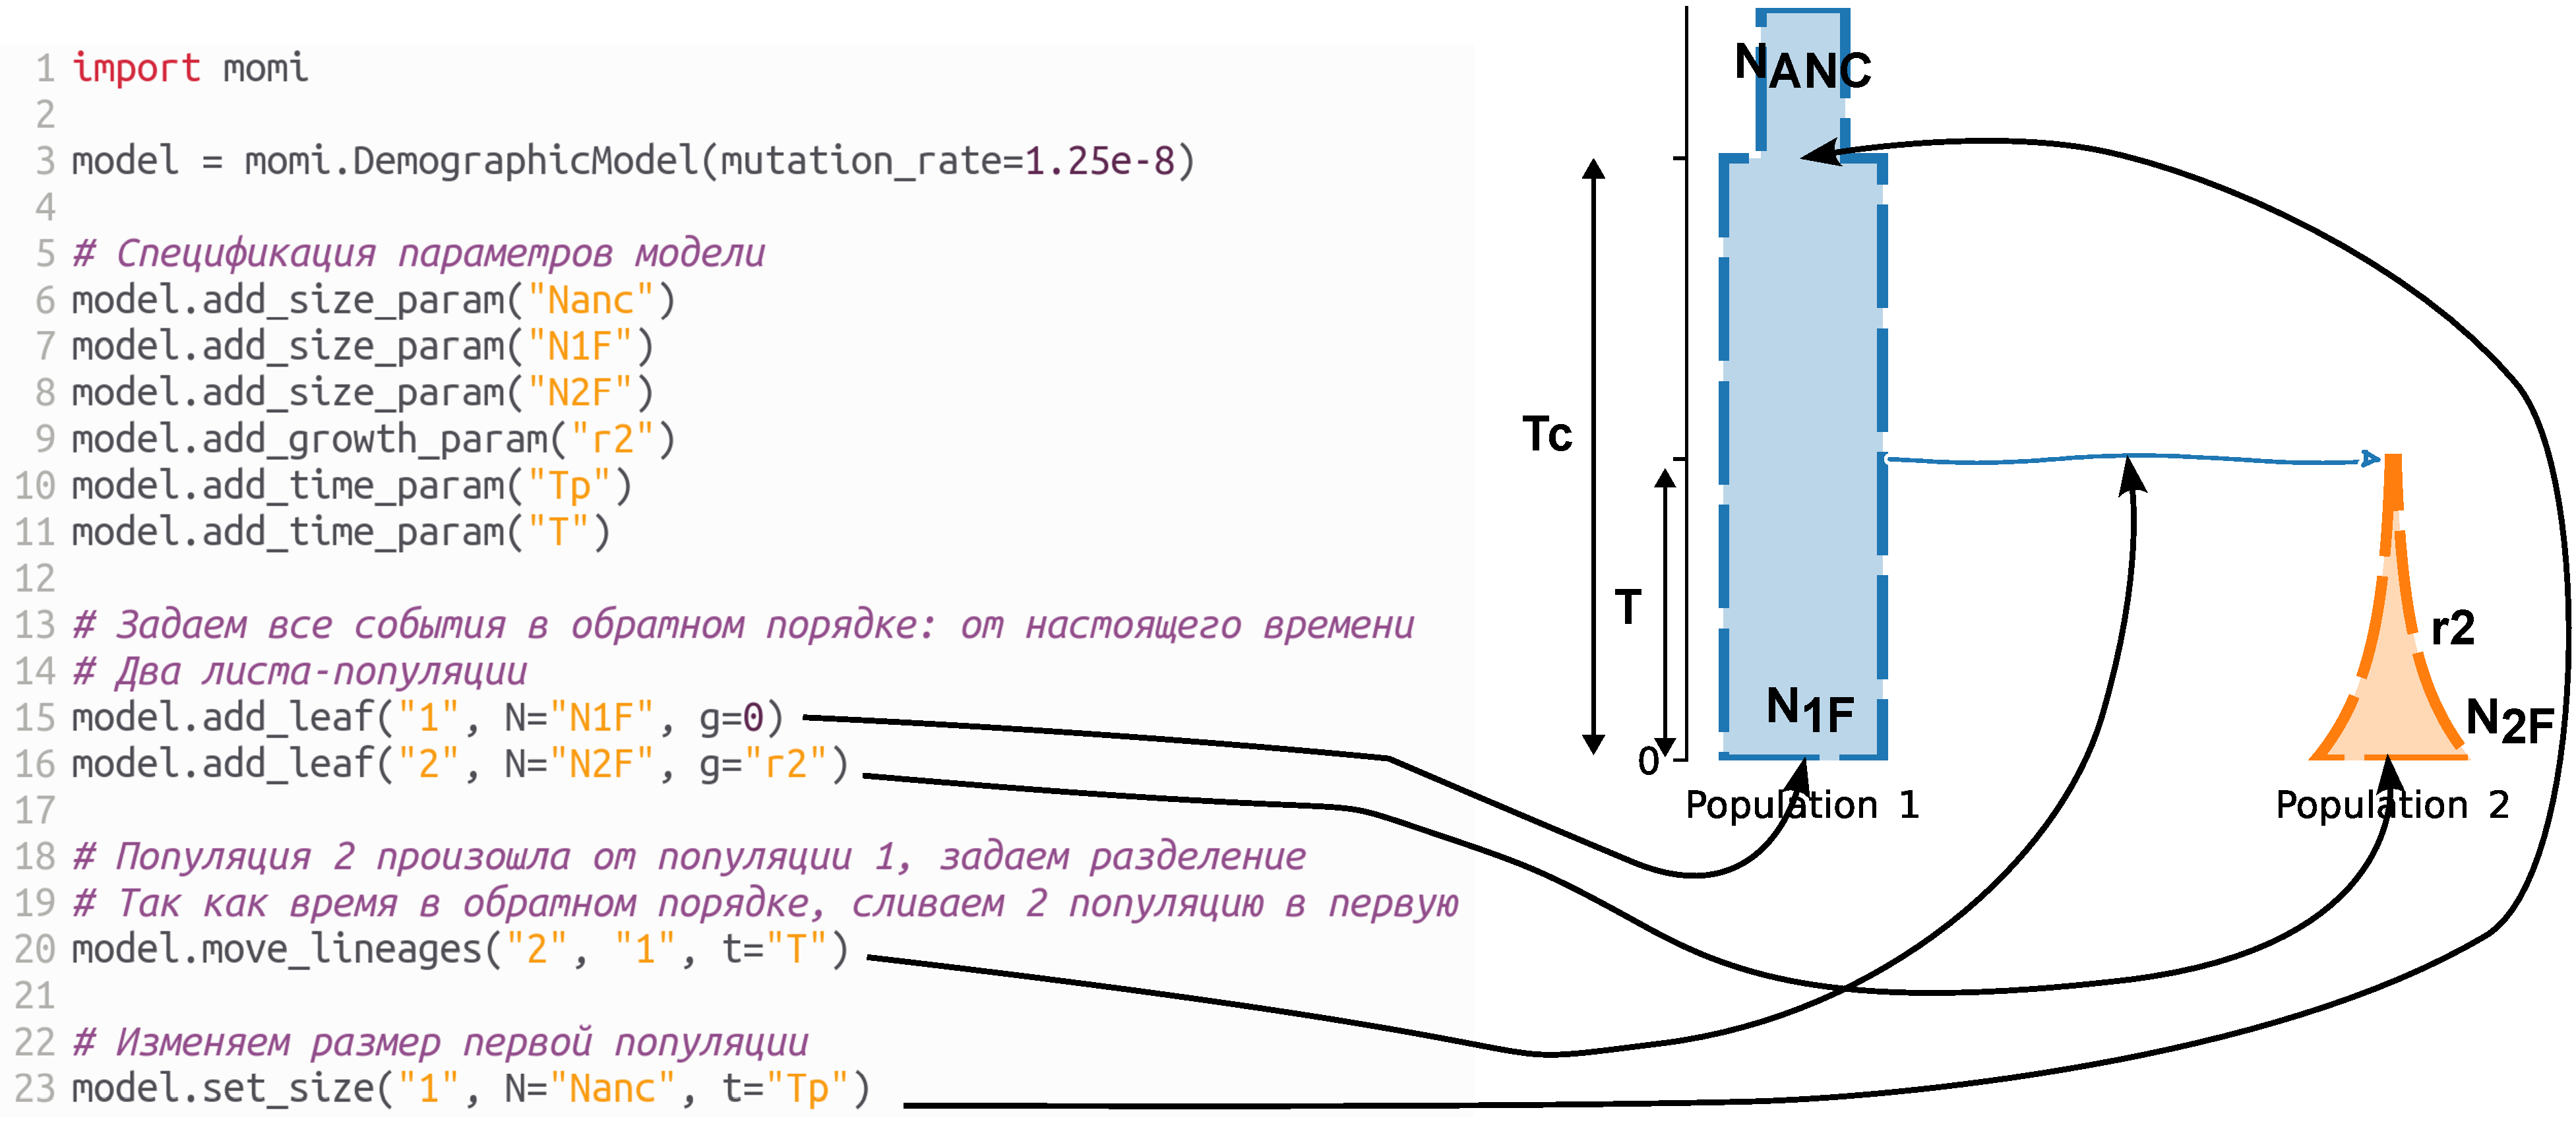
\includegraphics[width=\linewidth]{images_2/momi_model.pdf}
    \caption{Пример задания модели демографической истории с
использованием интерфейса библиотеки \momi}
    \label{fig:momi:model_spec}
\end{figure}

Эта библиотека также предоставляет метод локальной оптимизации для поиска параметров заданной модели.
Для получения более надежных результатов пользователь вынужден перебирать множество начальных точек и запускать локальную оптимизацию из каждой. 
Все численные методы для вычисления ожидаемых статистик данных и значения правдоподобия спрятаны в реализации процедуры \texttt{model.optimize} оптимизации.
Пример реализации алгоритма множественного запуска локальной оптимизации с использованием библиотеки \momi показан на рисунке~\ref{fig:momi:ls_run_several}.
\begin{figure}[h]
    \centering
    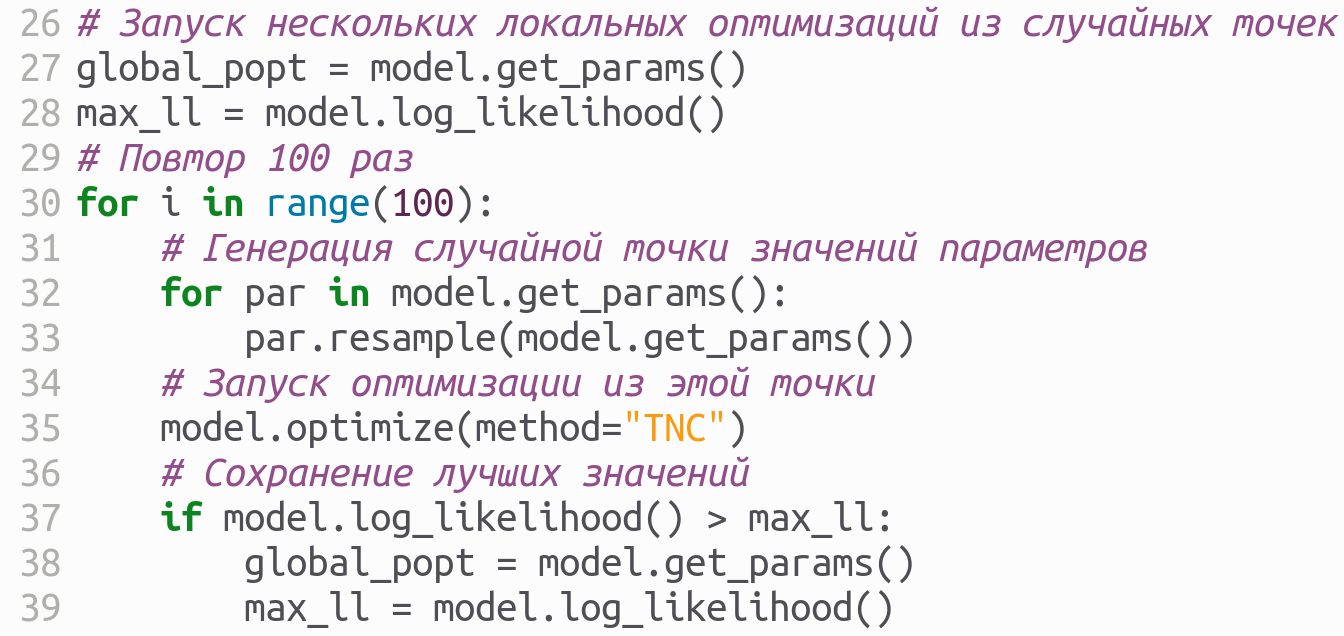
\includegraphics[width=0.6\linewidth]{images_2/momi_ls.png}
    \caption{Пример реализации алгоритма множественного запуска локальной оптимизации для поиска параметров модели с использованием \momi}
    \label{fig:momi:ls_run_several}
\end{figure}

\textbf{Выводы по обзору библиотеки \momi}

Недостатки моделей второго класса:
\begin{itemize}
    \item имеют только непрерывные параметры;
    \item динамики изменения численности (константная численность или экспоненциальное изменение) зафиксированы в модели;
    \item поддерживает только два закона изменения численности: константный и экспоненциальный. Невозможно, например, задать линейное изменение численности;
    \item порядок событий, таких как изменение численности или разделение популяций, не зафиксирован и может меняться в зависимости от значений параметров.\\
%    \item Спецификация экспоненциального изменения численности реализуется с использованием параметра степени экспоненциальной функции. Малые колебания значения этого параметра приводят к относительно большим колебаниям значений функции.
\end{itemize}

Недостатки использования библиотеки \momi для спецификации моделей:
\begin{itemize}
    \item позволяет работать только с моделями второго класса;
    \item позволяет использовать определенный набор параметров моделей (параметр численности, параметр времени, параметр степени экспоненциального изменения);
    \item каждая модель задается вручную с использованием специфичного интерфейса библиотеки \momi.
%    \item Модель нельзя переиспользовать. Модель, заданную с помощью библиотеки \momi, можно использовать только для вывода демографической истории с использованием \momi.
%    \item Динамики изменения численности (константная численность или экспоненциальное изменение) зафиксированы в модели.
%    \item Поддерживает только два закона изменения численности: константный и экспоненциальный. Невозможно, например, задать линейное изменение численности.
%    \item Порядок событий, таких как изменение численности или разделение популяций, не зафиксирован и может меняться в зависимости от значений параметров.
%    \item Спецификация экспоненциального изменения численности реализуется с использованием параметра степени экспоненциальной функции. Малые колебания значения этого параметра приводят к относительно большим колебаниям значений функции.
\end{itemize}

Недостатки использования библиотеки \momi для настройки значений параметров модели демографической истории:
\begin{itemize}
    \item пользователю требуется задавать и проверять каждую модель вручную с использованием библиотеки \momi;
    \item библиотека ограничена выводом значений только для непрерывных параметров;
    \item использование алгоритмов локальной оптимизации не гарантирует нахождение глобального оптимума.
\end{itemize}

% \begin{table}[h]
%     \centering
%     \begin{tabular}{|l|l|}
%         \hline
%         Модель & Недостатки-особенности \\
%         \hline
%         \dadi\ & 1. Требуется задание функций изменения численности. Для каждого \\
%         \moments& временного интервала и популяции в нем требуется вручную задать  \\
%         & функцию, при этом почти всегда используется небольшой набор \\
%         & функций. \\
%         & 2. Порядок событий таких как изменение численности и\\
%         & разделений популяций, зафиксирован. \\
%         & 3. Функция изменения численности зафиксирована и определяется \\
%         & непрерывными параметрами, такими, например, как численность \\
%         & популяции в начале и конце временного интервала. \\
%         & 4. Не универсальна --- может быть задана только для использования  \\
%         & в \dadi/\moments.\\
%         \hline
%         \momi & 1. Позволяет задать только константную численность или \\
%         & экспоненциальное изменение численности. Нет линейного изменения.\\
%         & 2. События могут «гулять» по времени, например, модель позволяет \\
%         & менять порядок событий изменения численности и разделений \\
%         & популяции в зависимости от значений параметров. \\
%         & 3. Малые изменения значения параметра степени экспоненциального \\
%         & изменения приводят к относительно большим изменениям размера \\
%         & популяции. \\
%         \hline
%     \end{tabular}
%     \caption{Недостатки-особенности описанных существующих моделей}
%     \label{tab:my_label}
% \end{table}

\subsubsection*{Обзор метода ручного перебора множества моделей для поиска демографической истории популяций}
%Для выбора модели исследователям приходится прибегать к перебору нескольких возможных моделей:
Напомним, что класс моделей, а также интерфейс библиотек \moments, \momentsLD совпадает с библиотекой \dadi.
Поэтому, хоть обзор программных включает только две библиотеки  \dadi и \momi, далее мы будем рассматривать четыре: \dadi, \moments, \momentsLD и \momi.

Для более надежного поиска демографической истории популяций пользователь использует не одну параметрическую модель, а несколько.
Для каждой модели настраиваются значения параметров и финальные демографические истории, соответствующие разным моделям с настроенными параметрами, сравниваются для выбора наилучшей.
Однако в таком методе перебор моделей происходит вручную самим пользователем.

Метод ручного перебора множества моделей состоит из следующих шагов (рисунок~\ref{fig:old_method:scheme}):
\begin{enumerate}
    \item Выбрать используемую библиотеку (\dadi, \moments, \momentsLD, \momi).
    \item Придумать набор возможных моделей демографической истории рассматриваемых популяций, которые отличаются набором параметров, законами изменения численности и деревом разделения (если рассматриваются более чем две популяции).
    \item Задать каждую модель с помощью используемой библиотеки.
    \item Реализовать программный код алгоритма поиска оптимальных параметров каждой модели.
    \item Для каждой модели выполнить поиск оптимальных значений параметров, дающих максимальное значение правдоподобия.
    \item Сравнить модели с разным числом параметров между собой, используя специальные метрики, например, статистический критерий Акаике~\myfootcite{akaike1974new}\myfootcite{coffman2016computationally}.\\
\end{enumerate}

\begin{figure}[h]
    \centering
    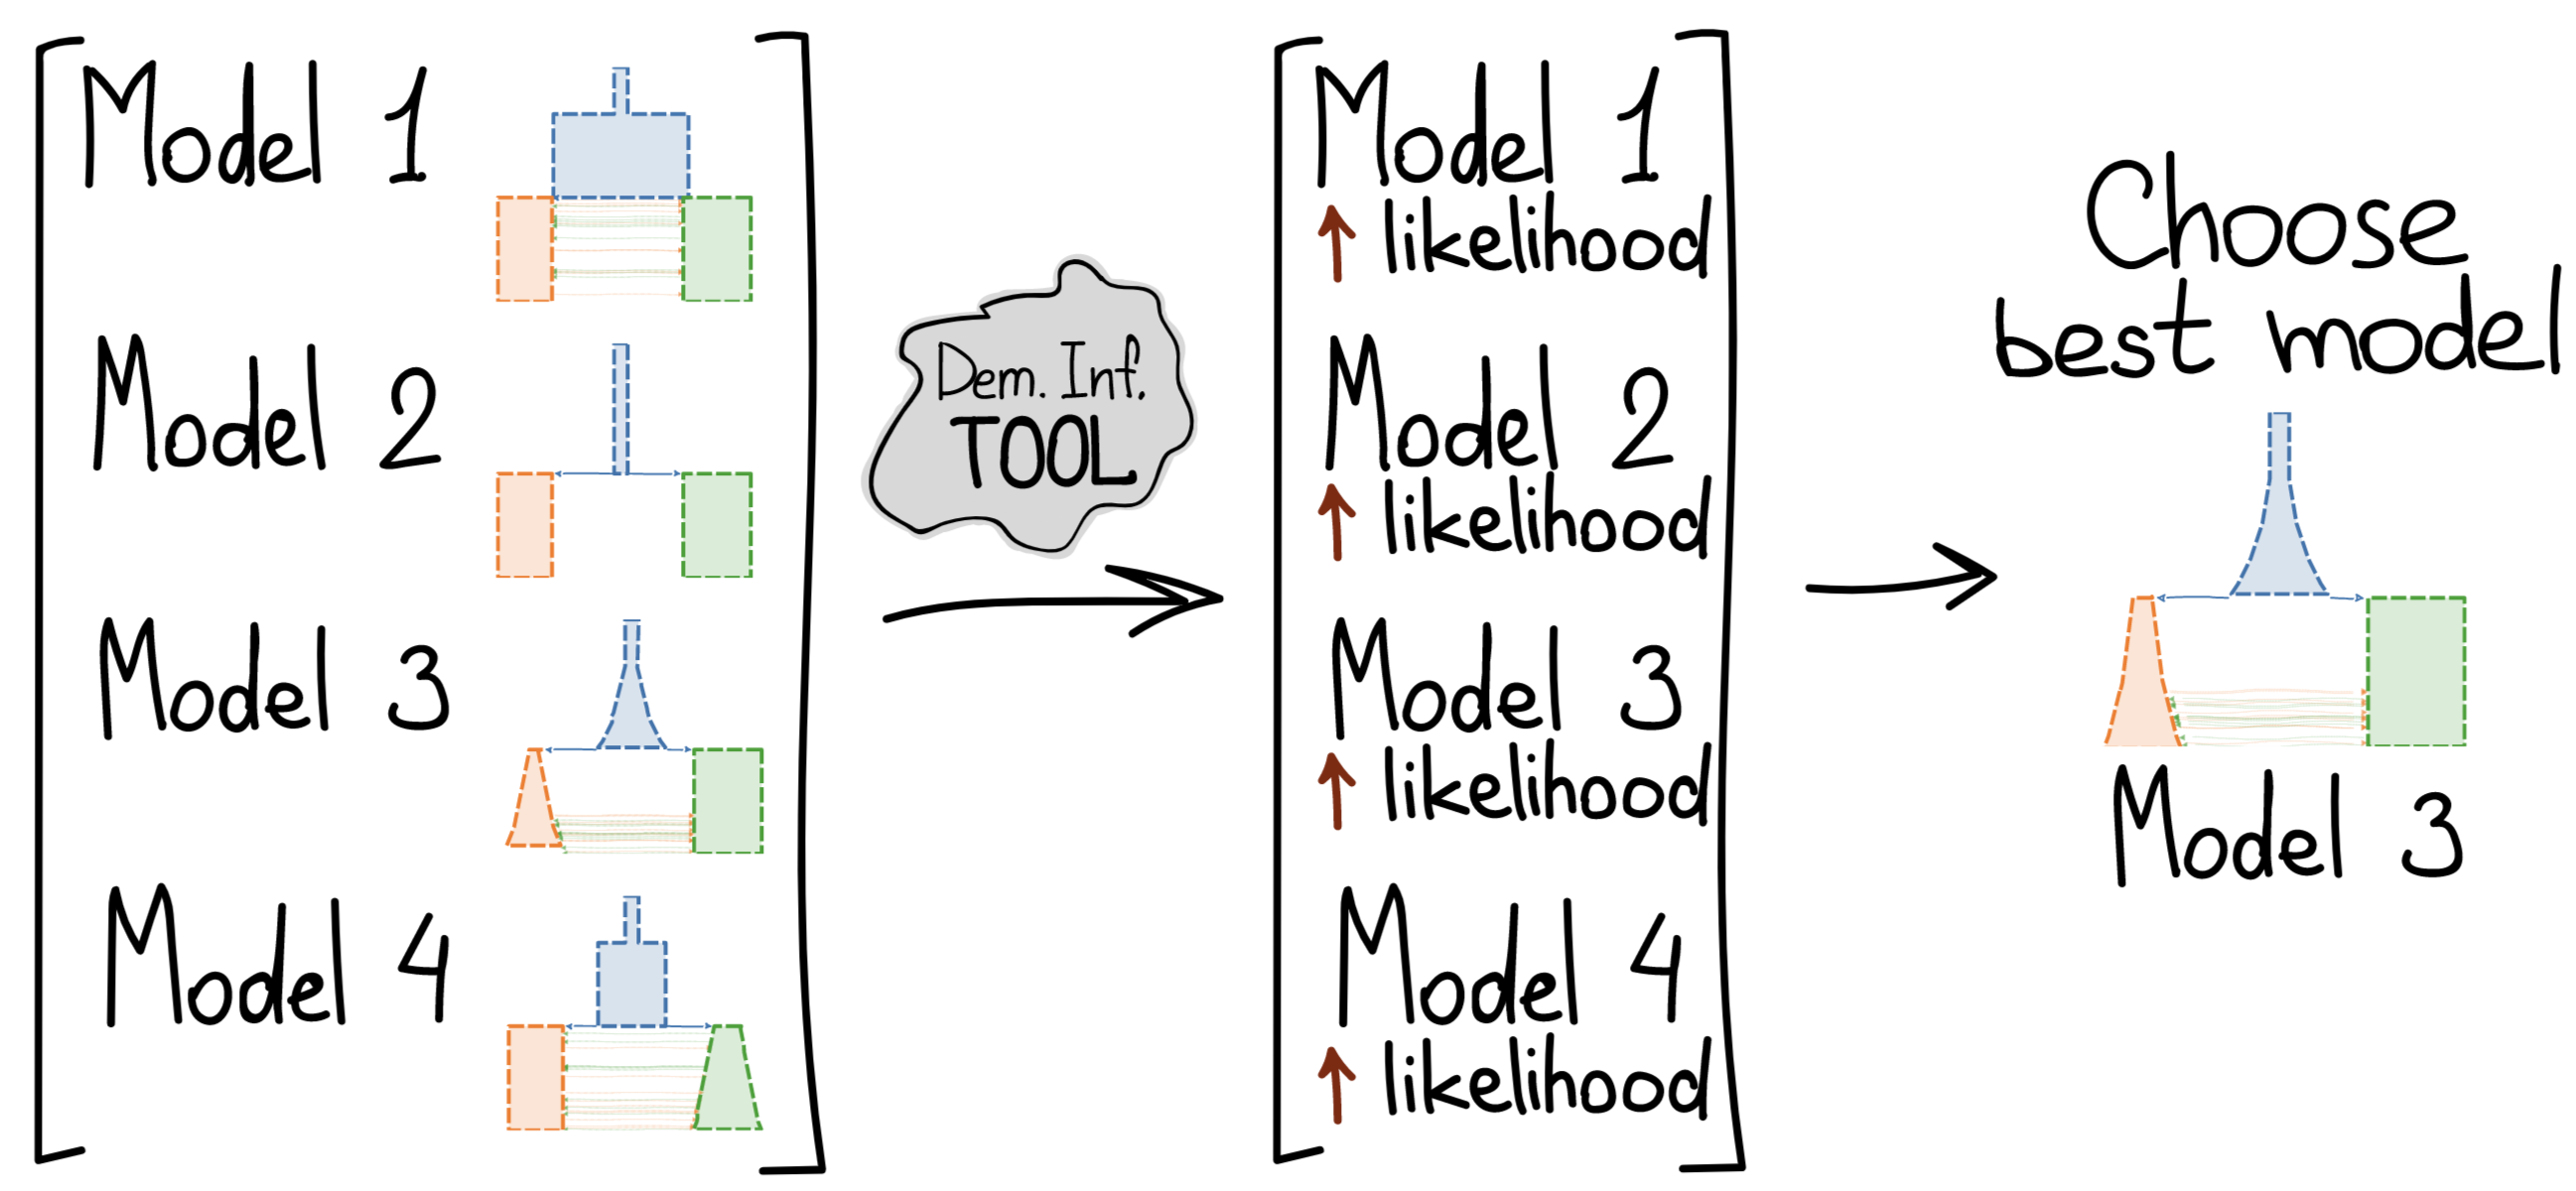
\includegraphics[width=\linewidth]{images_2/model_specifition.png}
    \caption{Общая схема метода ручного перебора множества моделей}
    \label{fig:old_method:scheme}
\end{figure}

Программные средства реализуют разные методы численного моделирования и поэтому имеют разные ограничения и стабильность работы.
Для получения более достоверных результатов пользователь может использовать несколько программных средств и сравнивать получаемые результаты.
Однако, такой подход требует задания одних и тех же моделей для каждого программного средства отдельно.\\

\newpage
\textbf{Выводы по обзору метода ручного перебора множества моделей}

Недостатки подхода, который заключается в использовании нескольких программных решений для поиска демографической истории популяций:
\begin{itemize}
    \item требуется задавать и тестировать множество похожих моделей, отличающихся только динамиками изменения численности;
    \item используются алгоритмы локального поиска, которые не гарантируют нахождения глобального оптимума.\\
\end{itemize}

Недостатки при использовании нескольких программных средств:
\begin{itemize}
\item возможно работать только с теми моделями, которые принадлежат пересечению классов моделей, поддерживаемых используемыми программными средствами;
\item требуется задавать одну и ту же модель каждый раз заново для каждого используемого программного средства.
\end{itemize}

\subsubsection*{Обзор методов автоматического перебора множества моделей для поиска демографической истории популяций}

На момент начала исследований не существовало метода автоматического поиска модели демографической истории популяций.
Все сравнения моделей с использованием информационного критерия Акаике~\myfootcite{akaike1974new}\myfootcite{coffman2016computationally} проводились пользователем в ручную, как было описано выше.

После публикации первой статьи~\myfootcite{noskova2020gadma} диссертанта появилось программное средство \texttt{AFS-analysis-with-moments}~\myfootcite{rippe2021environmental} для полуавтоматического перебора моделей с использованием библиотеки \moments.
Программное средство предоставляет каталог заранее реализованных моделей и позволяет выполнять настройку параметров моделей из каталога, используя локальную оптимизацию.
Однако оно ограничено рассмотрением только двух популяций.
Стоит отметить, что в последней версии программного средства \texttt{AFS-analysis-with-moments} локальный поиск был заменен глобальной оптимизацией, а именно генетическим алгоритмом, разработанным в данной работе.

\textbf{Выводы по обзору методов автоматического перебора множества моделей}

На момент начала исследований не существовало метода автоматического поиска модели демографической истории популяций.

Единственный метод-аналог, который появился после публикации статьи диссертанта, имеет следующие недостатки:
\begin{itemize}
    \item перебор моделей ограничен каталогом;
    \item позволяет автоматически перебрать модели только для демографической истории двух популяций.
\end{itemize}

\subsection*{Предложения автора}
\subsubsection*{Расширенный класс моделей}
Для упрощения работы пользователя биоинформатика был разработан расширенный класс моделей. 

Преимущества модели расширенного класса:
\begin{enumerate}
%    \item Заданная один раз модель быть переиспользована в любой из существующих библиотек: \dadi, \moments, \momentsLD, \momi.
    \item Включает новый тип параметров для вывода --- динамики изменения численности. При этом закон изменения численности в модели теперь может быть не фиксирован, а задан дискретным параметром, и его значение можно найти алгоритмом оптимизации.
\end{enumerate}

Приведем пример модели с параметром нового типа. Пусть модель на рисунке~\ref{fig:dadi:model_1} имеет дополнительный параметр \texttt{Dyn} --- динамика изменения второй популяции после разделения.
При разных значениях этого параметра численность второй популяции будет либо константная, либо будет иметь линейный или экспоненциальный закон изменения.
Изображение предложенной модели, а также демографические истории при разных значениях параметра \texttt{Dyn} показаны на рисунке~\ref{fig:new_model:model}.
\begin{figure}[h]
    \centering
    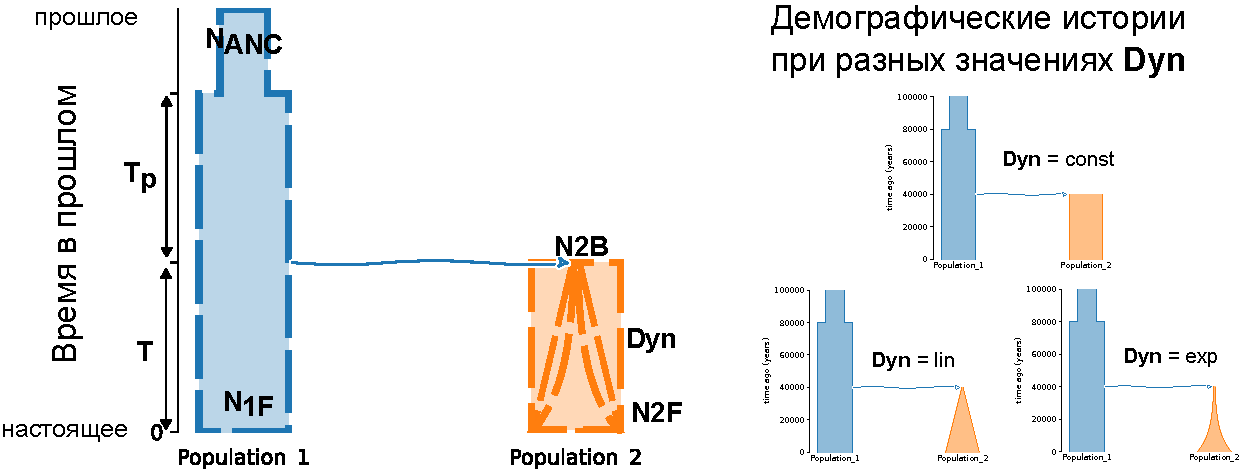
\includegraphics[width=\linewidth]{images_2/picture_2pops_model_3.pdf}
    \caption{Новая модель демографической истории с параметрами демографические истории при разных значениях параметра \texttt{Dyn}}
    \label{fig:new_model:model}
\end{figure}

В качестве прототипа расширенного класса моделей был выбран первый класс, в котором модели описываются временными интервалами и разделениями популяций.
Этот класс имеет больше преимуществ по сравнению со вторым классом, так как модели в нем могут описывать линейное изменение численности.

\definition Динамическими характеристиками $\chi_{dyn}(\mathcal{I})$ временного интервала $\mathcal{I} = <p, T, \mathfrak{N}^{start}, \mathfrak{N}^{end}, \mathfrak{d}>$ называется множество
$\{d_1, \cdots, d_p\}$.

\definition \textbf{Модель расширенного класса} для демографической истории $P$ популяций --- параметрическая модель для демографической истории $P$ популяций, которая представляется в виде пятерки $<\Theta, \Theta_d, \mathcal{E}, \mathfrak{F}, \mathfrak{F}_{d}>$, где $\Theta \subset \mathbb{R}_+^{k_1}$~---~множество значений непрерывных параметров модели, $\Theta_d \subset \{0, 1, 2\}^{k_2}$~---~множество значений дискретных параметров динамики, $\mathcal{E} = \{E_i\}_{i=1}^K,\ E_i \in \mathcal{I} \cup \mathcal{S}$~---~последовательность элементов временных интервалов и разделений, $\mathfrak{F}: \Theta \to  \bigcup \chi(E_i)$~---~отображение непрерывных параметров модели в характеристики элементов, $\mathfrak{F}_d: \Theta_d \to  \bigcup \chi_{dyn}(I_i),\ I_i \in \mathcal{E} \cap I$~---~отображение дискретных параметров динамики в динамические характеристики элементов временных интервалов.

\begin{figure}[h]
    \centering
    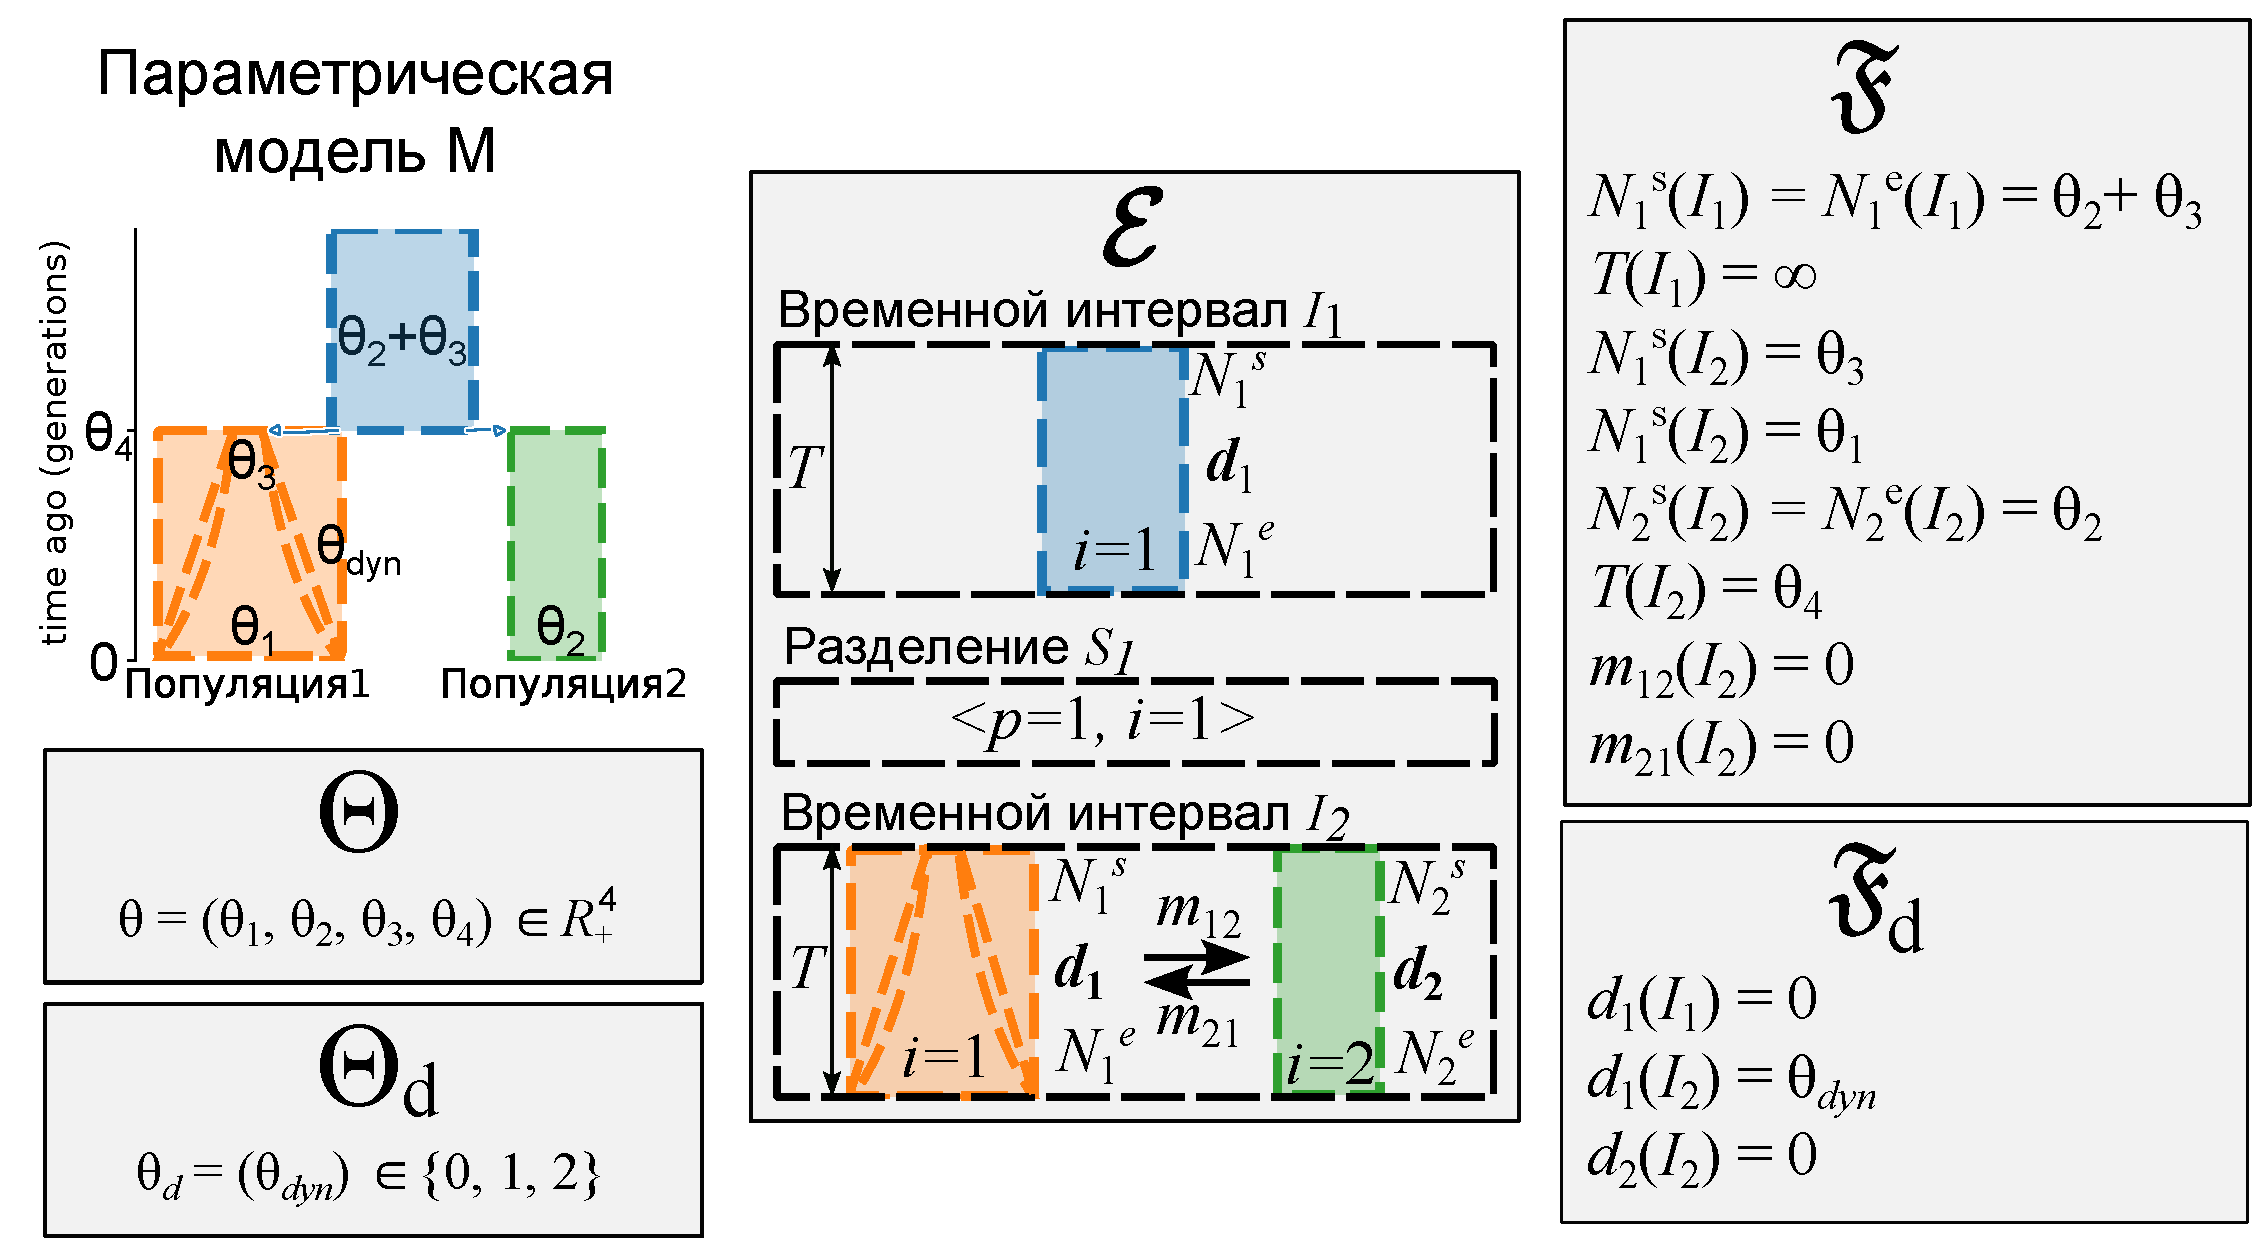
\includegraphics[width=\textwidth]{images_2/model_3_type.pdf}
    \caption{Пример модели $M = <\Theta, \Theta_d, \mathcal{E}, \mathfrak{F}, \mathfrak{F}_{d}>$ расширенного класса}
    \label{fig:model_3_type}
\end{figure}

%Мы опишем задание новой модели, используя понятие «характеристики».
%Каждая характеристика может являться либо параметром-переменной, либо комбинацией параметров-переменных, либо зафиксирована численным значением (константой).
% Для новой модели каждый временной интервал описывается следующими параметрами:
% \begin{itemize}
%     \item Время длительности интервала,
%     \item Размеры популяций в конце временного интервала,
%     \item (Опционально) размеры популяций в начале временного интервала. Если размеры не заданы, то они берутся как конечные размеры предыдущего интервала или разделения.
%     \item Динамики изменения численности, которые задают закон изменения численности соответствующей популяции и принимают одно из трех значений: константная численность, линейное или экспоненциальное изменение численности.
% \end{itemize}
% Элемент разделения популяции в модели описывается следующими параметрами:
% \begin{itemize}
%     \item Индекс разделяемой популяции,
%     \item Размеры разделяемой и новообразованной популяций после разделения.
% \end{itemize}

%Интерфейс для задания новой модели был реализован в программном комплексе GADMA.
Пример задания новой модели показан на рисунке~\ref{fig:new_model:model_spec}.
\begin{figure}[h]
    \centering
    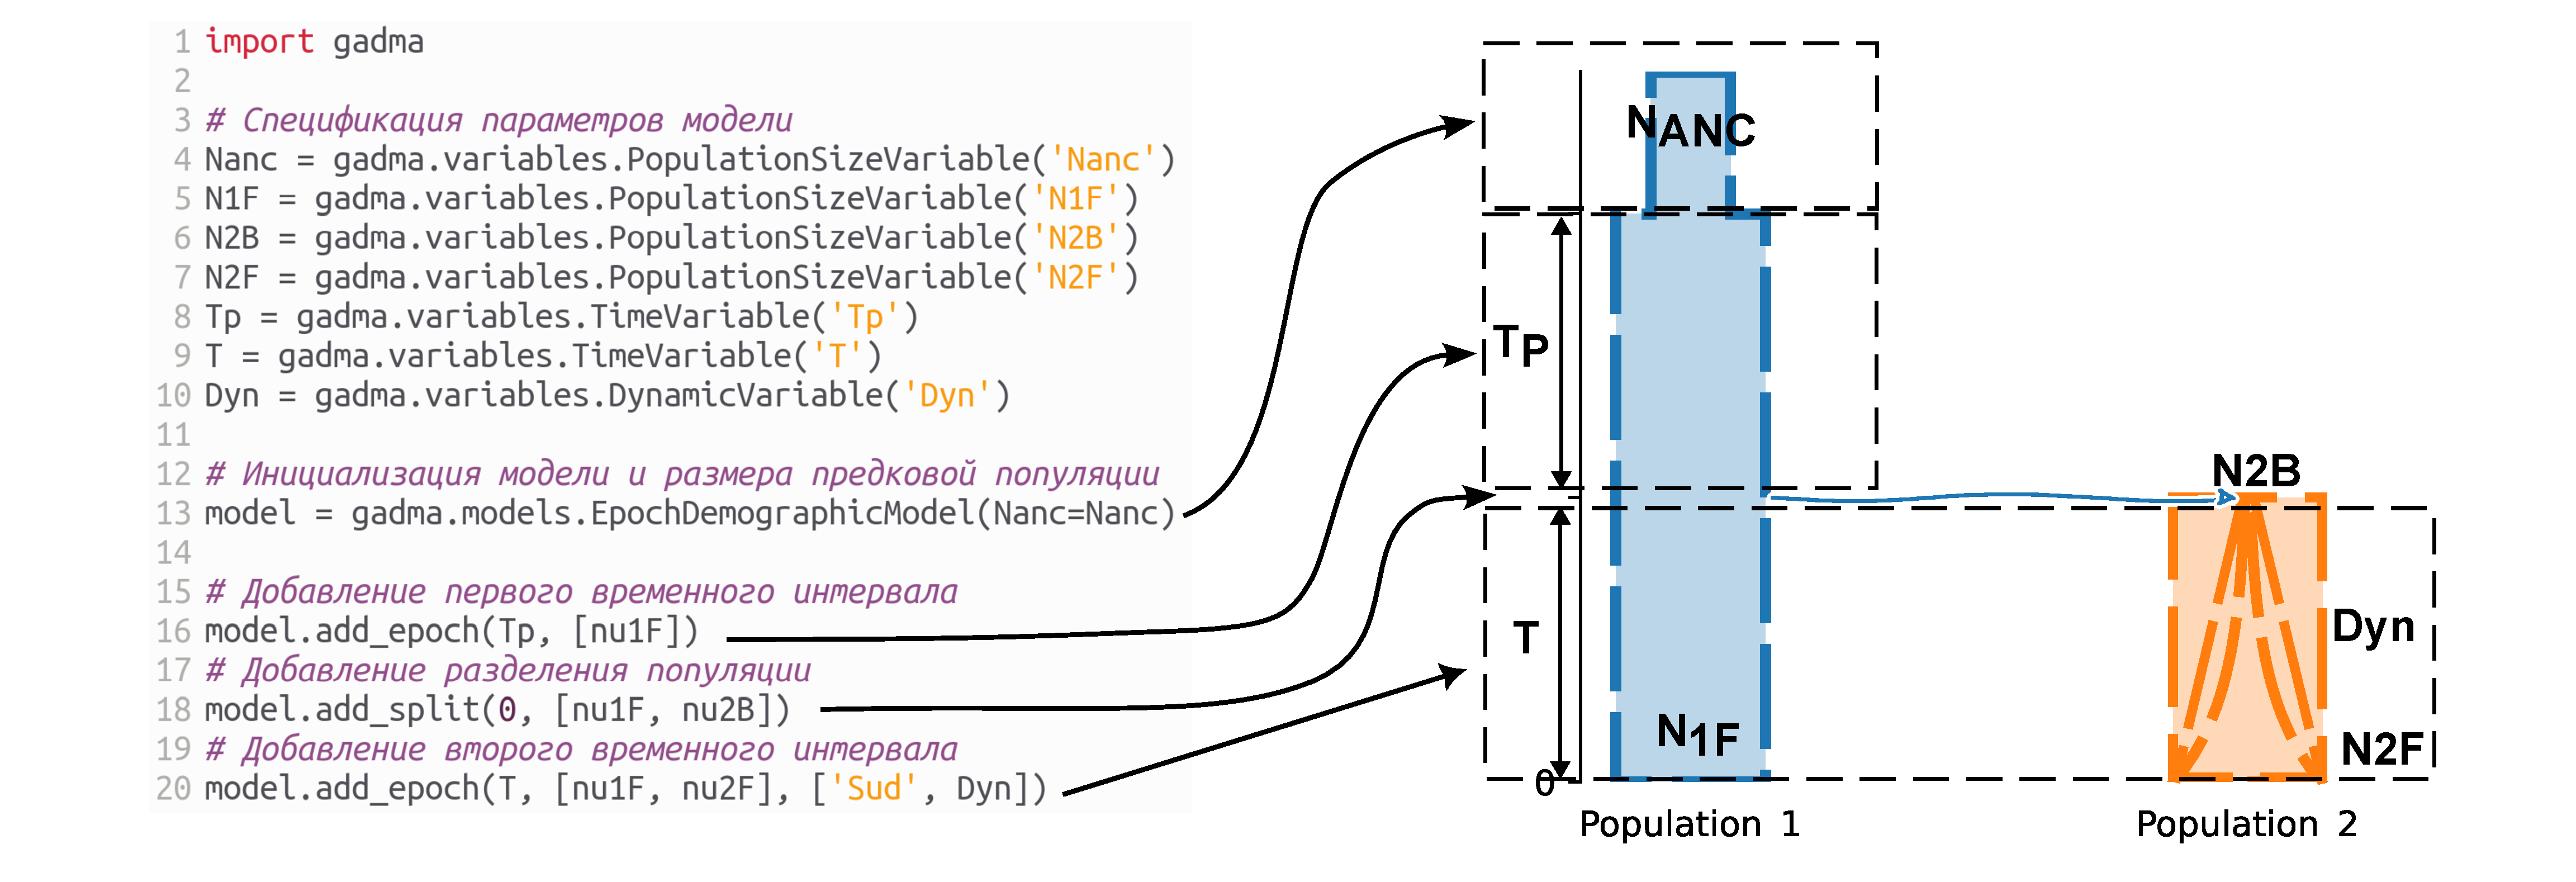
\includegraphics[width=\linewidth]{images_2/gadma_model.pdf}
    \caption{Пример задания расширенной модели}
    \label{fig:new_model:model_spec}
\end{figure}

Таким образом при использовании предлагаемой модели появляется возможность запуска алгоритма оптимизации для определения оптимальных законов изменения численности для любого временного интервала (в нашем примере только для второй популяции). Это позволит пользователю не перебирать разные модели вручную, как это требуется для \dadi, \moments, \momentsLD и \momi, а сделать это автоматически.

\subsubsection*{Методы глобальной оптимизации}

Для решения задачи настройки параметров расширенной модели демографической истории популяций, автором было разработано два метода глобальной оптимизации.
Первый метод, основанный на генетическом алгоритме, позволяет эффективно осуществить настройку параметров расширенных моделей для одной, двух и трех популяций.
Второй метод, основанный на байесовской оптимизации, выполняет эффективную настройку в случае более трех популяций.
Разработанные методы позволяют исключить необходимость задания начальных значений параметров и множественного запуска алгоритмов локальной оптимизации, а также способны выполнить поиск значений дискретных параметров, к которым относятся динамики изменения численности.

Сначала был разработан метод глобальной оптимизации, основанный на генетическом алгоритме, для поиска значений параметров модели, которые имеют максимальное значение правдоподобия.
Был разработан специальный вариант генетического алгоритма для рассматриваемой задачи, включающий несколько модификаций.
Более того, были подобраны оптимальные гиперпараметры генетического алгоритма.
Десять гиперпараметров алгоритма такие, как, например, число решений на одной итерации или сила изменения значения параметра, были автоматически найдены для наиболее эффективного решения поставленной задачи.

Однако временная сложность вычисления функции правдоподобия растет с увеличением числа рассматриваемых популяций.
Для некоторых программных решений таких, как \dadi и \moments, эта сложность растет экспоненциально.
%Из-за этого, генетический алгоритм эффективно решает поставленную задачу настройки параметров моделей не более чем для трех популяций.

Поэтому автором дополнительно был разработан метод, основанный на байесовской оптимизации, для настройки параметров моделей в условиях сложновычислимой функции правдоподобия.
Этот метод позволяет выполнить настройку параметров модели более эффективно, чем генетический алгоритм, в случае более трех популяций.
Гиперпараметры байесовской оптимизации такие, как ядро суррогатной модели и функция выбора, также были настроены для эффективного решения поставленной задачи.

На рисунке~\ref{fig:syn_ru:bo_ga_comp} представлен график сходимости разработанных методов при настройке параметров модели демографической истории пяти популяций.
Ось абсцисс соответствует времени работы методов в днях, ось ординат отображает расстояние до оптимума.
Байесовская оптимизация позволяет сократить время настройки на несколько дней, а иногда даже недель.

\begin{figure}[t!]
    \centering
    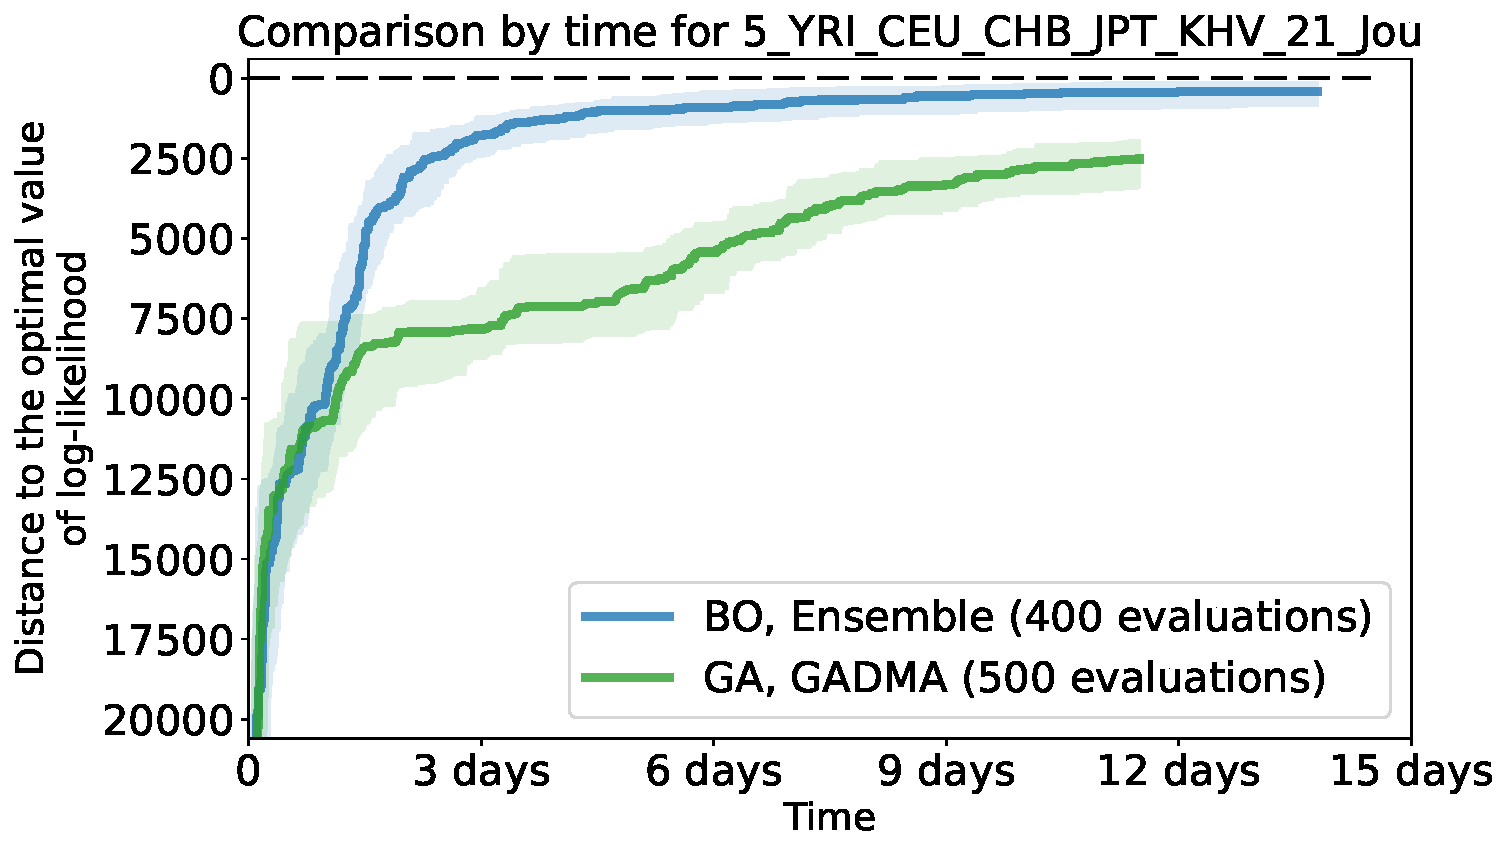
\includegraphics[width=0.6\textwidth]{images/bo_ga_comp_5_YRI_CEU_CHB_JPT_KHV_21_Jou.pdf}
    \caption{Сравнение сходимости методов байесовской оптимизации и генетического алгоритма}
    \label{fig:syn_ru:bo_ga_comp}
\end{figure}

Таким образом, у пользователя больше нет необходимости беспокоится о том, сколько раз запускать локальный поиск, из каких точек это делать --- автором предложено более эффективное и удобное в использовании решение.

\subsubsection*{Метод автоматического поиска оптимальной модели}

Следующим шагом в автоматизации всего процесса вывода демографической истории популяции является метод автоматического перебора расширенных моделей.
При этом пользователю необходимо будет лишь задать минимальные и максимальные ограничения на модель и метод самостоятельно выполнит перебор моделей в предоставленных границах.
Общая схема разработанного метода представлена на рисунке~\ref{fig:auto:scheme}.\\

На вход:
\begin{itemize}
    \item генетические данные;
    \item условия-ограничения для расширенных моделей.
\end{itemize}

На выход:
\begin{itemize}
    \item множество моделей, подходящих под условия-ограничения, и их настроенные значения параметров;
    \item выбор лучшей модели с использованием критерия Акаике~\myfootcite{akaike1974new}\myfootcite{coffman2016computationally}.\\
\end{itemize}

%Алгоритм выглядит следующим образом:
\begin{figure}[h!]
    \centering
    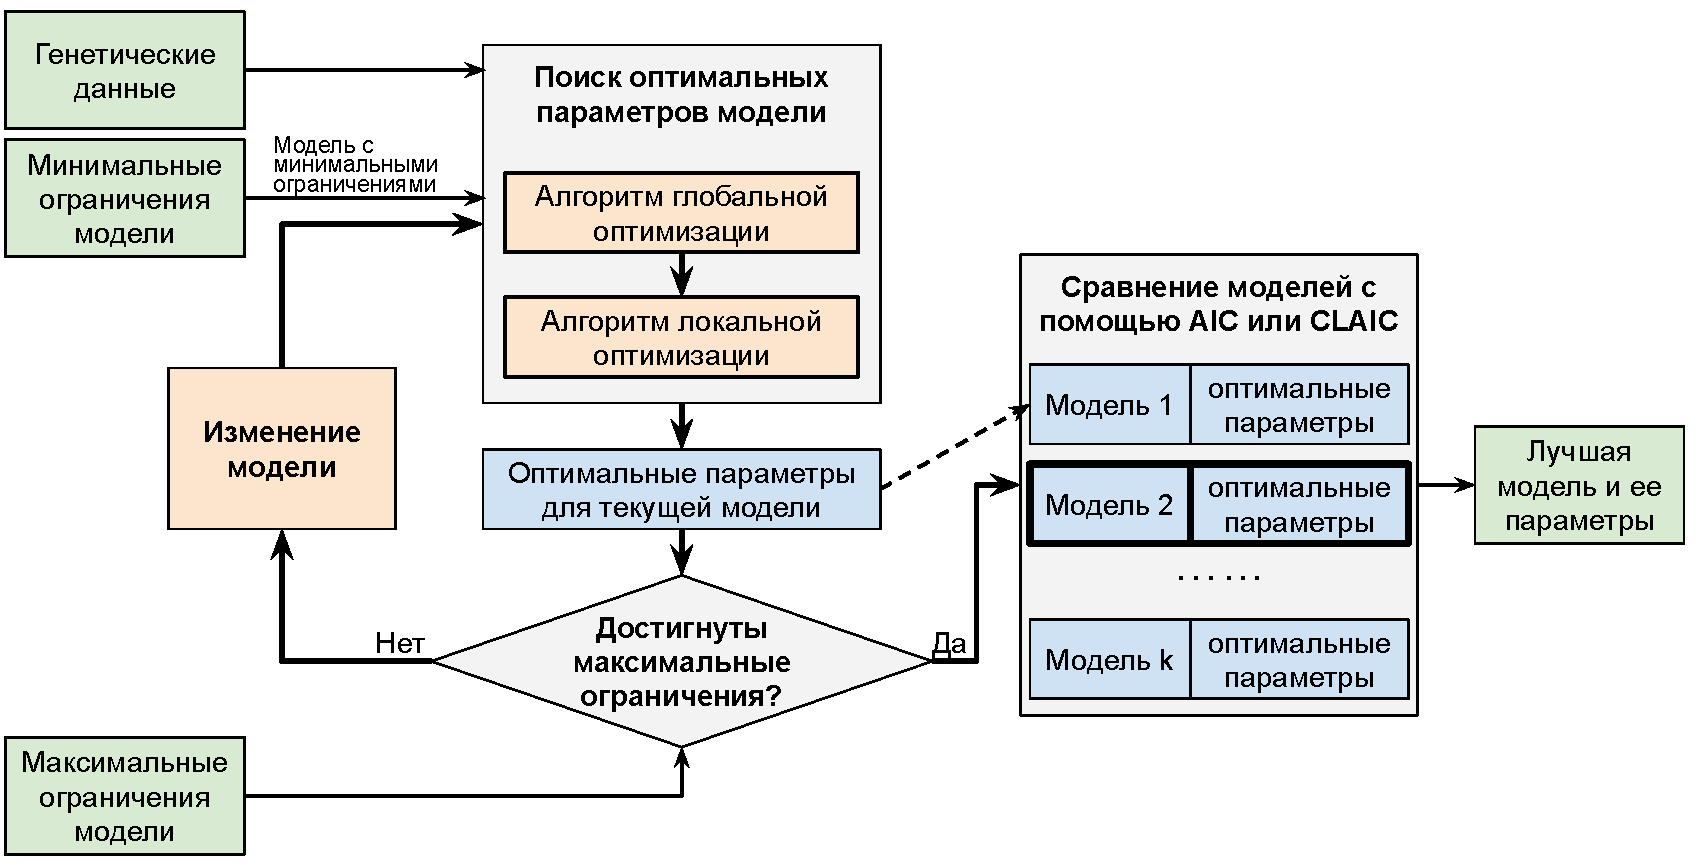
\includegraphics[width=0.9\linewidth]{images_2/general_scheme_rus.pdf}
    \caption{Схема разработанного метода автоматического перебора расширенных моделей демографической истории}
    \label{fig:auto:scheme}
\end{figure}

На каждой итерации разработанный метод использует комбинацию методов глобальной и локальной оптимизации для настройки параметров текущей модели.
В качестве алгоритма глобальной оптимизации предлагается использовать разработанный генетический алгоритм, в качестве локальной оптимизации можно использовать BFGS, метод Пауэлла или метод Нелдера-Мида.
Разработанный метод начинает с создания и настройки расширенной модели, которая удовлетворяет входным минимальным ограничениям.
Затем на каждой итерации текущая модель изменяется, увеличивается число ее параметров, и снова запускается процесс настройки ее параметров по генетическим данным.
При достижении максимальных ограничений на модели, метод останавливается и происходит сравнение всех перебранных моделей с помощью информационного критерия Акаике.
В результате работы, выбирается настроенная модель, которая наилучшим образом описывает генетические данные.
Таким образом, можно описать следующие шаги разработанного метода:
\begin{enumerate}
    \item Создать текущую модель, как модель с минимальными ограничениями.
    \item Найти оптимальные параметры для текущей модели по генетическим данным.
    \item Создать следующую модель, подходящую под ограничения.
    \item Повторить пункты б), в) пока не будут достигнуты максимальные ограничения.
    \item Сравнить множество перебранных моделей и выбрать лучшую.\\
\end{enumerate}

Для задания ограничений модели предлагается использовать число временных интервалов:
\begin{itemize}
    \item будем рассматривать максимум три популяции. В случае одной популяции в модели не будет разделения, в случае двух популяций будет одно разделение популяций и в случае трех популяций --- два разделения;
    \item будем задавать три числа $\{s_1, s_2, s_3\}$. Первое число определяет число временных интервалов до первого разделения (включая самый первый бесконечный интервал), второе число задает число временных интервалов между первым и вторым разделением, последнее третье число равно числу временных интервалов после второго разделения.
\end{itemize}
Минимальное ограничение --- это минимальное число временных интервалов в модели, максимальное ограничение --- это максимально возможное число временных интервалов в модели.

\definition Структура модели --- три числа $\{s_1, s_2, s_3\}$.\\

Для заданной структуры модель создается автоматически со всеми возможными параметрами, включая динамики изменения численности.

Структура включает три числа, так как наш метод расчитан только для одной, двух или трех популяций. Пример модели со структурой (2,1,1) представлен на рисунке~\ref{fig:auto:struct_2_1_1}.
\begin{figure}[h]
    \centering
    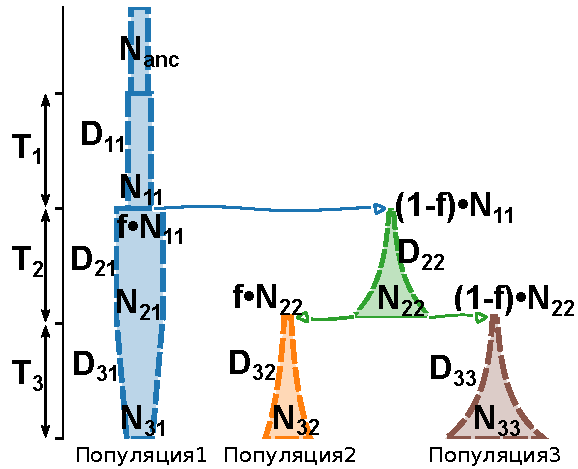
\includegraphics[width=0.6\linewidth]{images_2/struct_2_1_1.pdf}
    \caption{Пример модели трех популяций, которая соответствует структуре (2,1,1)}
    \label{fig:auto:struct_2_1_1}
\end{figure}

Пример модели двух популяций для структуры~(2,1,0) представлен на рисунке~\ref{fig:auto:struct_2_1_0}.
На рисунке~\ref{fig:auto:struct_2_1_0_ex} приведены демографические истории, которые соответствуют модели со следующими значениями параметров:
\begin{enumerate}
    \item \texttt{Nanc}: 7200, \texttt{T1}: 30000, \texttt{N11}: 40000, \texttt{D11}: Lin, \texttt{f}: $0.8$, \texttt{T2}: 50000, \texttt{N21}: 500, \texttt{N22}: 500, \texttt{D21}: Exp, \texttt{D22}: Sud;
    \item \texttt{Nanc}: 40000, \texttt{T1}: 50000, \texttt{N11}: 7000, \texttt{D11}: Sud, \texttt{f}: $0.1$, \texttt{T2}: 50000, \texttt{N21}:~5000, \texttt{N22}: 5000, \texttt{D21}: Lin, \texttt{D22}: Exp;
    \item \texttt{Nanc}: 7000, \texttt{T1}: 40000, \texttt{N11}: 20000, \texttt{D11}: Sud, \texttt{f}: 0.2, \texttt{T2}: 80000, \texttt{N21}:~20000, \texttt{N22}: 500, \texttt{D21}: Exp, \texttt{D22}: Lin.\\
\end{enumerate}

\begin{figure}[h]
    \centering
    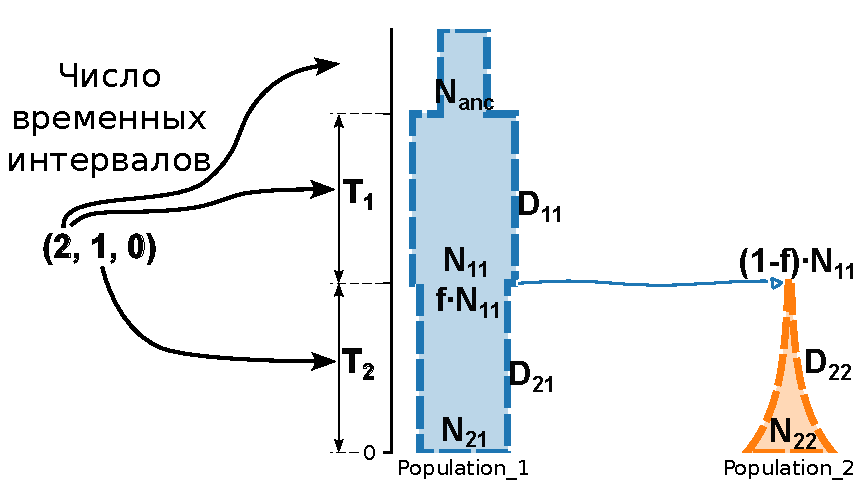
\includegraphics[width=0.6\linewidth]{images_2/picture_2pops_str_base.pdf}
    \caption{Пример модели двух популяций, которая соответствует структуре (2,1,0)}
    \label{fig:auto:struct_2_1_0}
\end{figure}

\begin{figure}[h]
    \centering
    \begin{subfigure}[c]{.32\textwidth}
    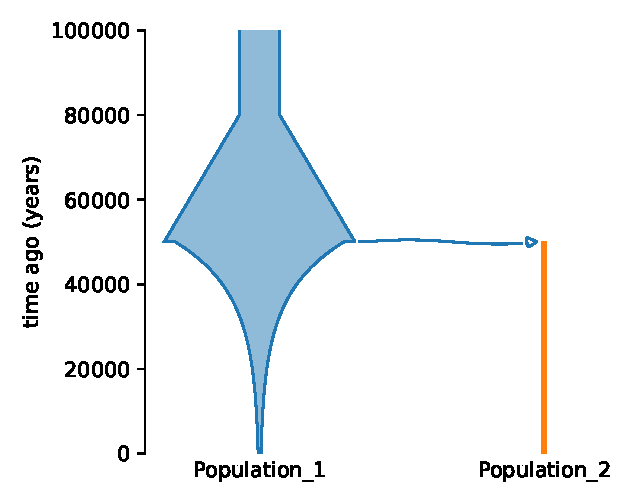
\includegraphics[width=\textwidth]{images_2/picture_2pops_str_2.pdf}
    \caption{}
    \label{fig:auto:struct_2_1_0_ex_1}
    \end{subfigure}%
    \begin{subfigure}[c]{.32\textwidth}
    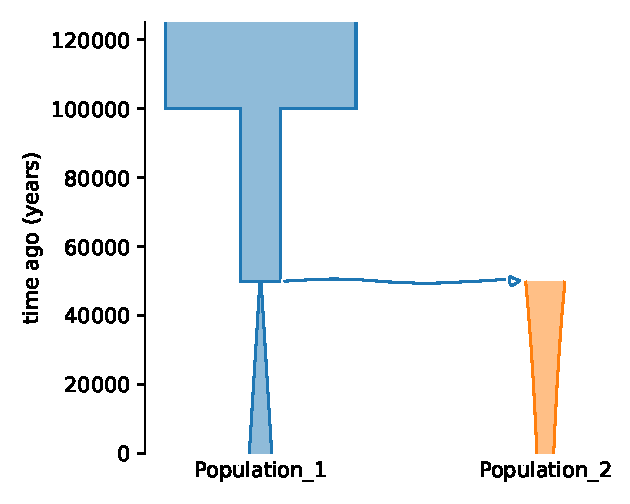
\includegraphics[width=\textwidth]{images_2/picture_2pops_str_3.pdf}
    \caption{}
    \label{fig:auto:struct_2_1_0_ex_2}
    \end{subfigure}%
    \begin{subfigure}[c]{.32\textwidth}
    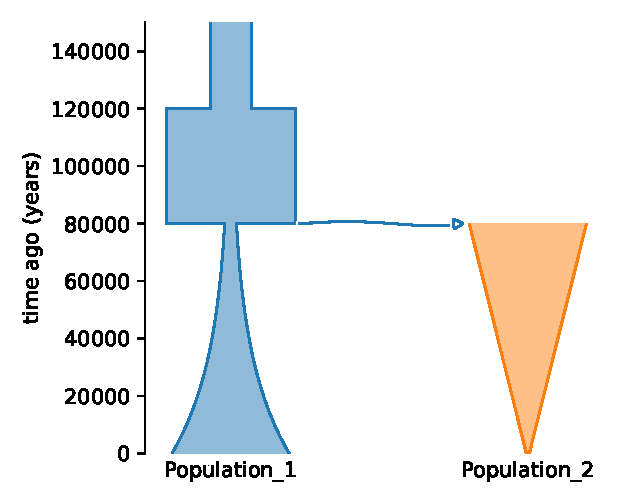
\includegraphics[width=\textwidth]{images_2/picture_2pops_str_4.pdf}
    \caption{}
    \label{fig:auto:struct_2_1_0_ex_3}
    \end{subfigure}
    \caption{Демографические истории для модели со структурой (2,1,0) при разных значениях ее параметров}
    \label{fig:auto:struct_2_1_0_ex}
\end{figure}

Для изменения модели в разработанном методе автоматического перебора, автором был предложен метод увеличения числа временных интервалов в структуре модели:
\begin{itemize}
    \item из трех частей временной оси (до первого разделения, между первым и вторым разделениями, после второго разделения) случайным образом выбрать часть, где еще не достигнуто финальное число временных интервалов;
    \item случайным образом выбрать временной интервал в части;
    \item разделить временной интервал на две части, создать новые параметры, вычислить их значения в соответствии со значениями старых параметров.\\
\end{itemize}

Опишем разработанный метод автоматического перебора моделей с использованием структур.
На первом шаге создается модель с начальной структурой и осуществляется настройка ее параметров.
Затем на каждом последующем шаге увеличивается число временных интервалов в структуре модели и производится поиск параметров для модели с большим числом параметров.
Процесс завершается, когда найдены оптимальные параметры для модели с заданной финальной структурой.
На последнем шаге происходит сравнение моделей с разными структурами с использованием статистического критерия Акаике.\\

Вход:
\begin{itemize}
    \item генетические данные;
    \item начальная структура модели;
    \item финальная структура модели.
\end{itemize}

Выход:
\begin{itemize}
    \item оптимальные значения параметров для моделей с разной структурой;
    \item информация о лучшей модели при сравнении с использованием информационного критерия Акаике.
\end{itemize}


\subsubsection*{Программный комплекс GADMA}

Все разработанные методы и предложенная модель были использованы автором при разработке программного комплекса GADMA (Global search Algorithm for Demographic Model Analysis).
Исходный код GADMA находится в открытом доступе на GitHub под лицензией GPLv3: \url{https://github.com/ctlab/GADMA}.
Программный комплекс обладает общедоступной документацией, расположенной по ссылке: \url{https://gadma.readthedocs.io}.
Все компоненты программного комплекса автоматически тестируются с использованием системы непрерывной интеграции GitHub Actions.
Когда программный код GADMA обновляется в любой ветви репозитория, то запускается процесс тестирования, и программное средство тестируется на различных платформах: Linux, Windows и macOS.

GADMA включает в себя выбор из «движков» \dadi, \moments, \momi --- методов для вычисления функции правдоподобия, и имеет методы как глобальной, так и локальной оптимизации для настройки параметров моделей.
Более того, GADMA включает метод автоматического перебора моделей в заданных ограничениях.
Структура программного комплекса представлена на рисунке~\ref{fig:syn_ru:gadma_modules}.

\begin{figure}[h]
    \centering
    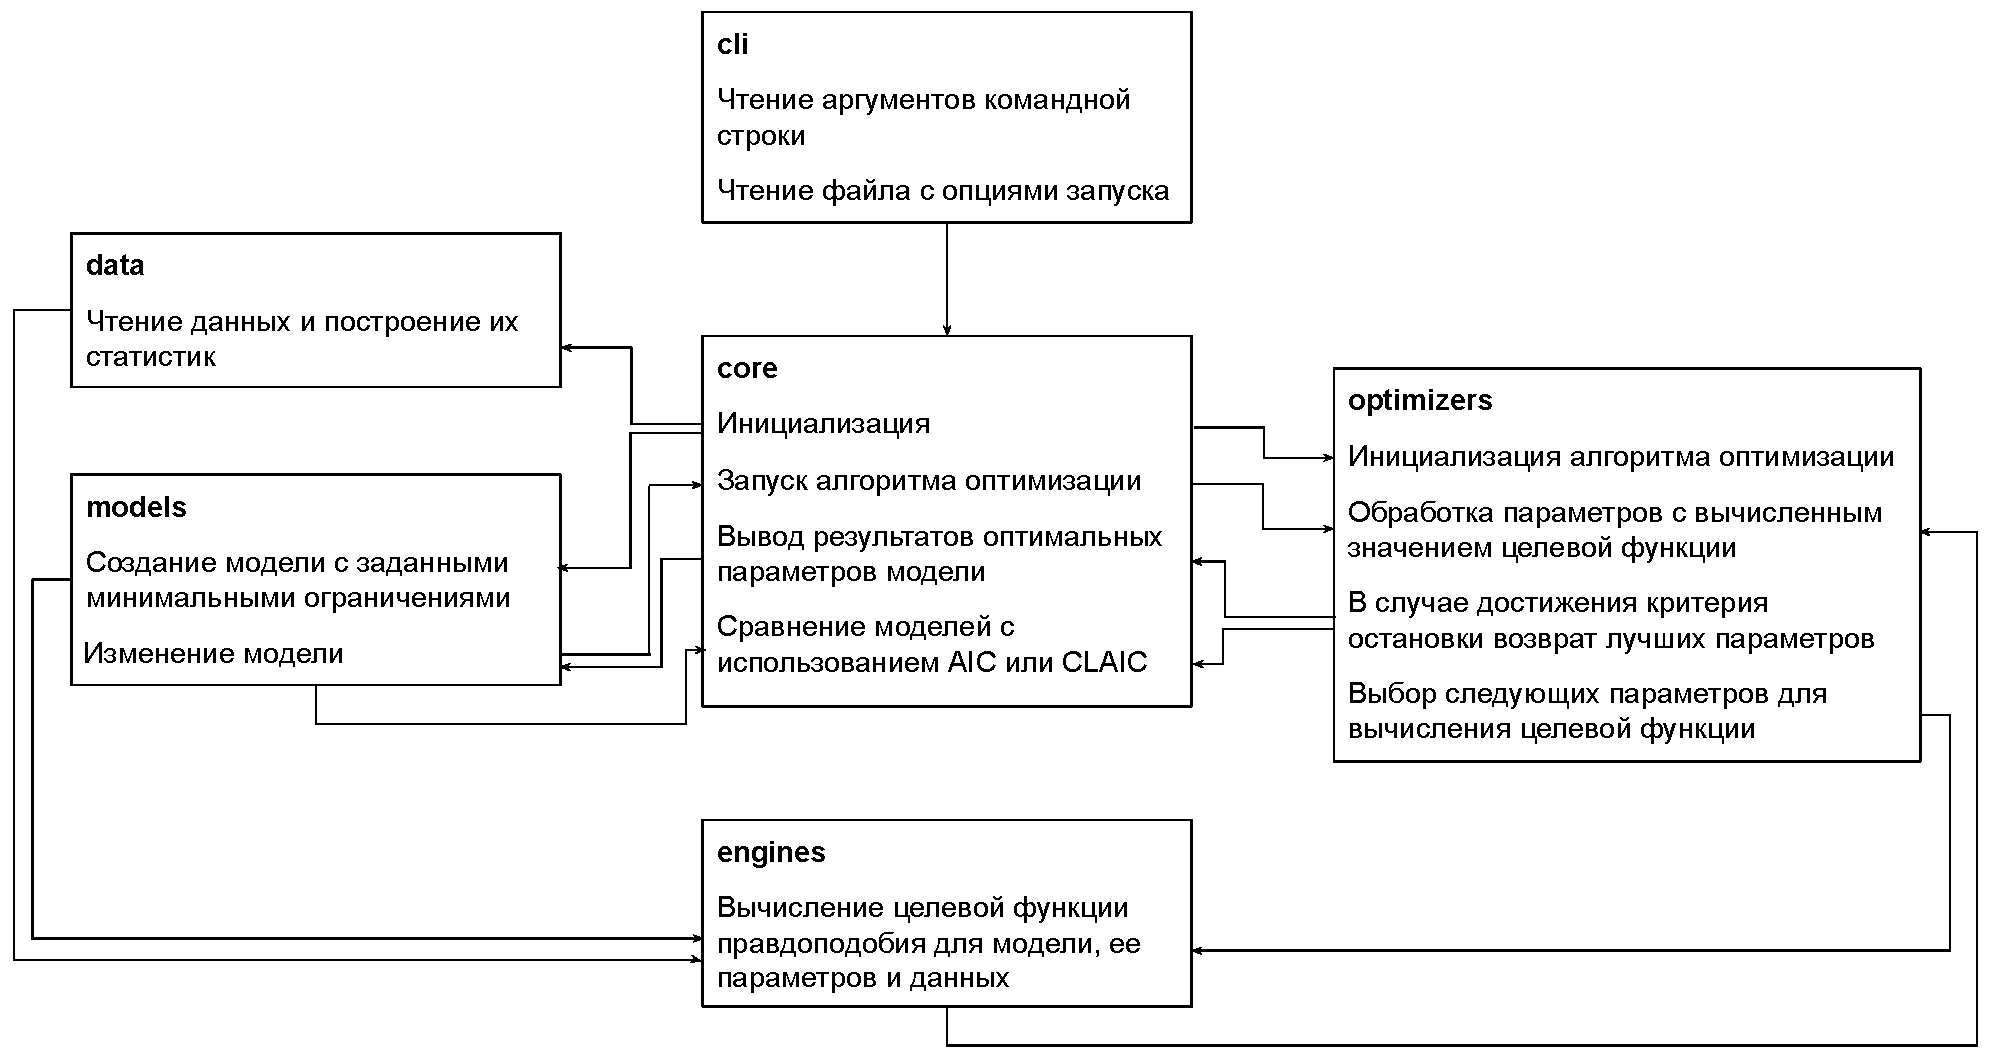
\includegraphics[width=\linewidth]{images/part5/gadma_modules.pdf}
    \caption{Структура программного комплекса GADMA}
    \label{fig:syn_ru:gadma_modules}
\end{figure}

Модель демографической истории в GADMA может задаваться любым способом, однако, универсальная спецификация только одна --- для разработанной автором расширенной модели.
Ранее, для использования нескольких программных средств требовалось задать спецификацию модели используя интерфейсы каждого программного средства.
Используя спецификацию GADMA для расширенной модели, можно один раз задать модель, а затем одним изменением названия движка (\texttt{Engine}) в файле с опциями найти оптимальные параметры сначала для \dadi, потом для \moments, затем для \momentsLD, а потом и для \momi.

Пример файла с опциями GADMA для настройки параметров заданной расширенной модели приведен на рисунке~\ref{fig:gadma_params}.

\begin{figure}[h]
    \centering
    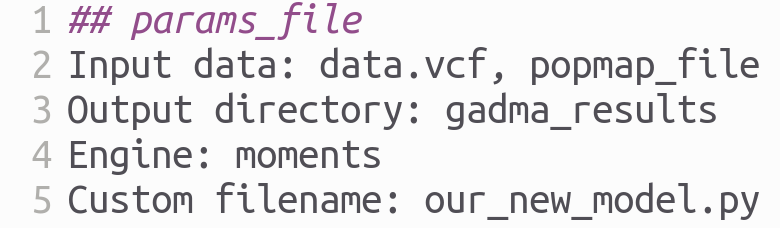
\includegraphics[width=0.5\linewidth]{images_2/gadma_file.png}
    \caption{Пример файла с опциями GADMA для настройки параметров модели}
    \label{fig:gadma_params}
\end{figure}

Этот файл \texttt{params\_file} специфицирует по строкам: 2) файл с данными, 3) папку вывода, 4) используемый движок --- moments, 5) файл с заданной новой моделью.

Запуск GADMA для настройки параметров модели:
$$\text{\texttt{\$ gadma -p params\_file}}$$

В качестве результата на экран пользователю на каждой строке будет выведена следующая информация:
\begin{enumerate}
    \item номер запуска (можно запустить несколько запусков параллельно);
    \item максимально найденное значение правдоподобия;
    \item значения параметров, названия параметров указываются в скобках.\\
\end{enumerate}

Пример вывода для одной популяции:
$$\text{Run 1   -95.95  [ [Nanc = 7729],        [ 2806.55(t1), [2745.65(nu11)], [Exp(dyn11)] ] ] }$$

Кроме настройки параметров заданной модели, программный комплекс GADMA позволяет выполнить автоматический поиск модели демографической истории.
Пример файла с опциями GADMA для поиска оптимальной модели демографической истории приведен на рисунке~\ref{fig:gadma_str_params}.
\begin{figure}[h]
    \centering
    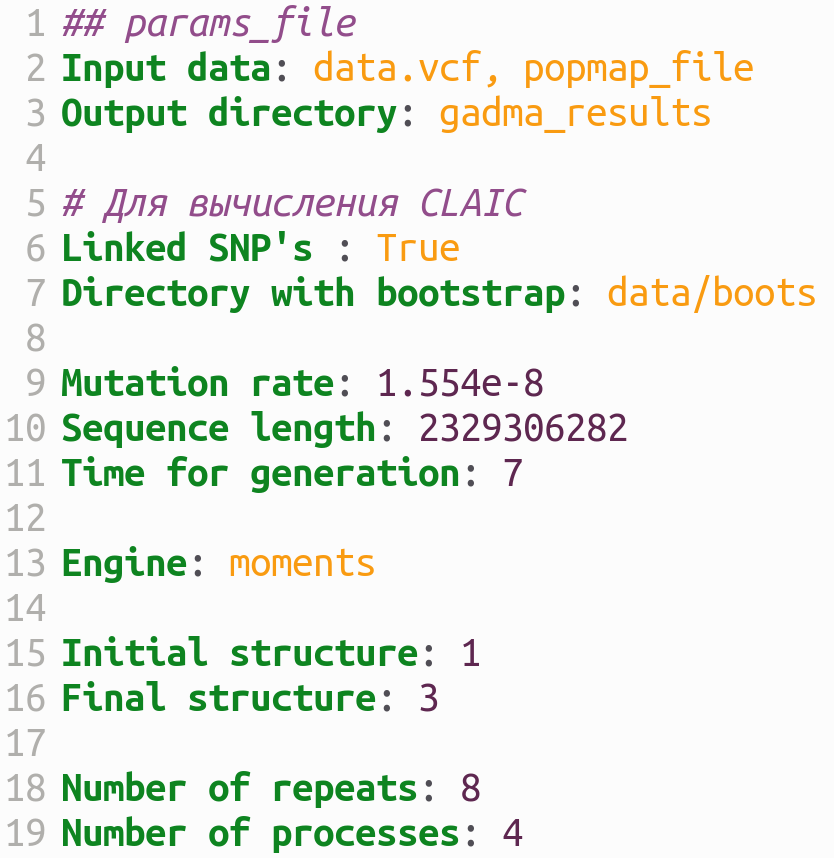
\includegraphics[width=0.5\linewidth]{images_2/gadma_str_params_file.png}
    \caption{Пример файла с опциями для запуска GADMA для автоматического перебора моделей}
    \label{fig:gadma_str_params}
\end{figure}

Этот файл \texttt{params\_file} специфицирует по строкам: 2) файл с данными, 3) папку вывода, 6-7) данные для вычисления информационного критерия Акаике, 9-11) характеристики рассматриваемых популяций, 13) используемый движок --- moments, 15) минимальное ограничение на число временных интервалов модели, 16) максимальное число интервалов в модели, 18-19) общее число запусков и число процессов для их параллелизации.

Запуск GADMA для автоматического перебора моделей:
$$\text{\texttt{\$ gadma -p params\_file}}$$

В качестве результата на экран пользователю будет выведен список перебранных моделей с настроенными парамтрами, отсортированные по значению информационного критерия Акаике. Пример вывода для одной популяции приведен на рисунке~\ref{fig:gadma_str_output}.
GADMA выводит два списки настроенных моделей: 1) с наилучшими значениями правдоподобия, 2) с наилучшими значениями информационного критерия Акаике.

\begin{figure}[h]
    \centering
    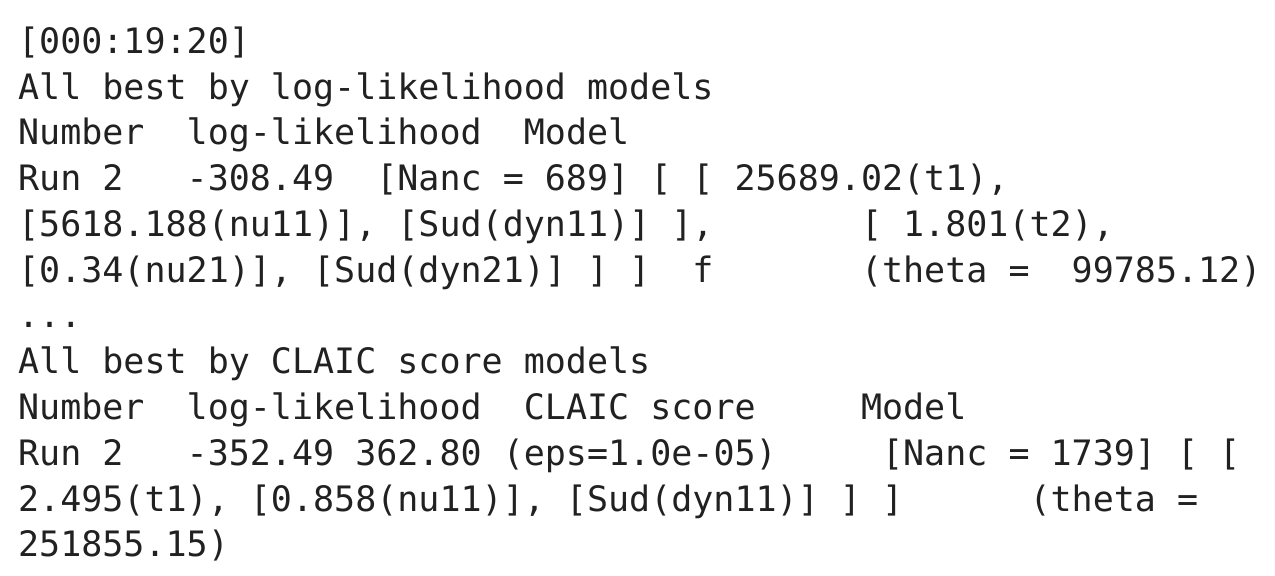
\includegraphics[width=0.7\linewidth]{images_2/gadma_str_output.png}
    \caption{Пример вывода GADMA при автоматическом переборе моделей}
    \label{fig:gadma_str_output}
\end{figure}

\newpage
\subsection*{Положения, выносимые на защиту, обладающие научной новизной}

\begin{itemize}
    \item расширенный класс моделей демографической истории популяций, содержащий, как и аналоги, модели с непрерывными параметрами, отличающийся тем, что с целью расширения пространства поиска он дополнительно включает модели с дискретными параметрами динамики изменения численности популяций;
    \item метод настройки параметров расширенных моделей по заданными генетическими данными, содержащий существующие методы численного моделирования, и отличающийся тем, что с целью поиска глобального оптимума используются методы глобальной оптимизации, а именно генетический алгоритм и байесовская оптимизация;
    \item метод автоматического перебора расширенных моделей с разным числом параметров и настройки их параметров по генетическим данным одной, двух и трех популяций, отличающийся тем, что с целью повышения уровня автоматизации  и обеспечения возможности настраивать не только параметры модели, но и саму модель демографической истории, он включает метод увеличения числа временных интервалов модели;
    %Метод автоматического перебора расширенных моделей с разным числом параметров и настройки их параметров по генетическим данным, отличающийся уровнем автоматизации и позволяющий настраивать не только параметры модели, но и саму модель демографической истории.
%    \item Программный комплекс для поиска демографической истории популяций по генетическим данным, содержащий существующие методы вычисления функции правдоподобия, отличающийся тем, что с целью повышения уровня автоматизации и уменьшения экспертных знаний о модели у конечного пользователя, дополнительно содержит методы глобальной оптимизации и метод автоматического перебора моделей.
    %Программный комплекс для поиска демографической истории популяций по генетическим данным, отличающийся повышенным уровнем автоматизации и требующим меньших экспертных знаний о модели от конечного пользователя.
\end{itemize}

\subsection*{Положение, выносимое на защиту, являющееся практическим результатом}

\begin{itemize}
\item программный комплекс для поиска демографической истории популяций по генетическим данным, содержащий существующие методы вычисления функции правдоподобия, отличающийся тем, что с целью повышения уровня автоматизации и уменьшения экспертных знаний о модели у конечного пользователя, дополнительно содержит методы глобальной оптимизации и метод автоматического перебора моделей.
    %Программный комплекс для поиска демографической истории популяций по генетическим данным, отличающийся повышенным уровнем автоматизации и требующим меньших экспертных знаний о модели от конечного пользователя.
\end{itemize}

\subsection*{Соответствие специальности 1.2.2 «Математическое моделирование, численные методы и комплексы программ»}

В паспорте специальности указано:\\
\textit{*Диссертационное исследование должно содержать все три составляющих названия специальности}

В работе есть:
\begin{itemize}
    \item методы математического моделирования \textbf{в части} новой модели и методов ее моделирования на основе данных натурного эксперимента;
    \item численные методы \textbf{в части} используемых методов для вычисления функции правдоподобия, а также \textbf{в части} метода статистического критерия Акаике в условиях зависимости данных;
    \item комплекс программ \textbf{в части} реализации всех методов в программном комплексе GADMA.
\end{itemize}

%\textbf{Пункт 1.} (Разработка новых математических методов моделирования объектов и явлений (физико-математические науки)) не подходит, так как у нас не физ-мат?

\textbf{Пункт 2 паспорта специальности.} (Разработка, обоснование и тестирование эффективных вычислительных методов с применением современных компьютерных технологий) 
Мы разработали, обосновали и протестировали два эффективных вычислительных метода: 1) метод настройки параметров расширенных моделей демографической истории по заданным генетическим данным, 2) метод автоматического перебора оптимальной модели демографической истории.
%Здесь еще можно сказать, что метод сравнения моделей с разным числом параметров, а именно CLAIC --- это численный метод, мы реализуем алгоритм, который сравнивает модели с использованием CLAIC.

%\textbf{Пункт 3.} (Реализация эффективных численных методов и алгоритмов в виде комплексов проблемно-ориентированных программ для проведения вычислительного эксперимента) можем ли мы говорить, что наша комбинация вычислительных методов для вычисления правдоподобия и методов глобальной оптимизации --- это реализация эффективным численных методов и алгоритмов?
%Здесь еще можно сказать, что метод сравнения моделей с разным числом параметров, а именно CLAIC --- это численный метод, мы реализуем алгоритм, который сравнивает модели с использованием CLAIC.

\textbf{Пункт 4  паспорта специальности.} (Разработка новых математических методов и алгоритмов интерпретации натурного эксперимента на основе его математической модели)
Разработанные методы моделируют демографическую историю популяций по генетическим данных (данные натурного эксперимента).

%\textbf{Пункт 5.} (Разработка новых математических методов и алгоритмов валидации математических моделей объектов на основе данных натурного эксперимента или на основе анализа математических моделей) подходит

%\textbf{Пункт 8.} (Комплексные исследования научных и технических проблем с применением современной технологии математического моделирования и вычислительного эксперимента) все то же что и предыдущие два?

\textbf{Пункт 9  паспорта специальности.} (Постановка и проведение численных экспериментов, статистический анализ их результатов, в том числе с применением современных компьютерных технологий (технические науки))
Разработка единого программного комплекса GADMA позволила провести множество вычислительных экспериментов по выводу демографических историй популяций по генетическим данным.
Результаты проведенных вычислительных экспериментов были проанализированы, а именно различные модели были сравнены с использованием статистических методов таких, как информационный критерий Акаике и тест отношения правдоподобий.


\subsection*{Апробация результатов работы}

Основные результаты работы были представлены на следующих международных конференциях:

\begin{itemize}
    \item Международный конгресс «VII съезд Вавиловского общества генетиков и селекционеров, посвященный 100-летию кафедры генетики СПбГУ, и ассоциированные симпозиумы», 2019, Санкт-Петербург, Россия;
    \item Moscow Conference on Computational Molecular Biology, 2019, Москва, Россия;
    \item Probabilistic Modeling in Genomics, 2019, Осуа, Франция;
    \item Probabilistic Modeling in Genomics, 2021, онлайн;
    \item Moscow Conference on Computational Molecular Biology, 2021, Москва, Россия;
    \item Probabilistic Techniques in Analysis, 2021, Сочи, Россия;
    \item Conservation Genomics at the Population Level, 2022, Кембридж, Великобритания;
    \item LI Научная и учебно-методическая конференция Университета ИТМО, 2022, Университет ИТМО, Санкт-Петербург, Россия;
    \item XI Конгресс молодых ученых, 2022, Университет ИТМО, Санкт-Петербург, Россия;
    \item Probabilistic Modeling in Genomics, 2022, Окфорд, Великобритация;
    \item XII Конгресс молодых ученых, 2023, Университет ИТМО, Санкт-Петербург, Россия;
    \item Probabilistic Modeling in Genomics, 2023, Колд Спринг Харбор, США;\\
\end{itemize}

\subsection*{Награды}

\begin{itemize}
    \item Бронзовая награда в номинации 17th Human-Competitive Awards на онлайн конференции The Genetic and Evolutionary Computation Conference (GECCO) в 2020 году.
    \item Победитель конкурсной программы поддержки исследовательских проектов System Biology Fellowship от Сколковского института науки и технологий по проекту «Computational methods for unsupervised demographic inference of multiple populations from genomic data» в 2021 году.
\end{itemize}


\begin{refsection}
\nociteallauthorpublications
\newrefcontext[sorting=none] % sort references as they are set
\urlstyle{rm}\printauthorpublications\urlstyle{tt}
\newpage
\end{refsection}

% \subsection*{Предложение по изменению структуры диссертации}

% В целях соответствия диссертации специальности 1.2.2 предлагается внести следующие изменения в структуру:

% \begin{enumerate}
%     \item Вынести метод автоматического поиска модели демографической истории популяций в начало, как первую главу.
%     \item В первой главе сделать акцент на разработке новой модели для описания демографической истории популяций. Пример этого описания (без миграций) представлен ниже в этом документе.
%     Обозначить метод перебора новых моделей как разработанный метод математического моделирования.
%     \item Для генетического алгоритма и байесовской оптимизации сделать акцент на их применение в комбинации с разработанным методом поиска модели.
%     \item Сделать дополнительный акцент на численных методах, использующихся в существующих методах вычисления функции правдоподобия.
% \end{enumerate}

% \newpage
% \subsection*{Приложение: математический аппарат}

% % При поиске демографической истории популяции \textbf{приходится прибегать к использованию модели} --- параметризованному семейству демографических историй, которое позволяет ограничить пространство для поиска.
% % Конфигурация модели --- это набор параметров модели, а также связей между ними, то есть ее структура.

% % Существует множество методов и программных решений для вывода демографической истории популяций по генетическим данным.
% % Эти методы включают в себя \textit{комбинацию алгоритмов имитационного моделирования, численных методов и методов оптимизации}.
% % Они \textbf{требуют заданную исследователем модель демографической истории} на вход и осуществляют поиск оптимальных параметров этой модели.
% % \textbf{Эти модели включают только непрерывные параметры, такие как время или размер популяции, и всегда имеют зафиксированные функции изменения численности.}
% % Методы имитационного моделирования и численные методы используются для вычисления функции правдоподобия демографической истории и данных натурного эксперимента.
% % Именно эта величина определяет оптимальность параметров и используется в качестве целевой функции в алгоритмах оптимизации.
% % Кроме того, в подавляющем большинстве методов классические \textbf{алгоритмы локальной оптимизации} используются для поиска параметров заданной модели.
% % Эти алгоритмы \textit{требуют начальной оценки параметров} и их эффективность сильно зависит от этого выбора.

% % Также \textbf{каждое программное средство имеет свой собственный способ и интерфейс для задания конфигурации модели}, что вызывает дополнительные трудности при применении нескольких программ.
% % Для улучшения точности и достоверности вывода, исследователь вынужден рассматривать \textbf{целое множество возможных конфигураций}, задавать каждую из них \textbf{вручную}, находить оптимальные значения параметров и сравнивать результаты между собой.
% % Этот процесс требует значительных временных затрат, тем больше, чем больше рассматриваемых популяций, а также опыта в области изучаемых видов.
% % %Кроме того, неверный выбор начальных оценок параметров моделей может снизить эффективность используемого алгоритма оптимизации и привести к недостоверным результатам при сравнении моделей.

% % Все это ограничивает возможности существующих подходов к выводу демографической истории популяций.
% % Создание новой универсальной модели упростит процесс использования программных решений.
% % А метод автоматического подбора оптимальной конфигурации модели также значительно усовершенствует современные подходы.

% % \subsection*{Описание новых разработанных математических моделей демографической истории популяции}

% % В начале мы кратко приведем описание разработанных моделей демографической истории.
% % Более подробное описание с примерами задания приведены ниже.
% % Мы разработали две новые модели демографической истории.

% % Первая модель имеет следующие характеристики:
% % \begin{itemize}
% %     \item Введен новый параметр --- динамика изменения численности популяций, которая может быть константной, линейной или экспоненциальной. Модель включает такие динамики, как дискретные параметры для вывода. В ранее существующих моделях функции изменения численности были всегда зафиксированы.
% %     \item Каждая такая новая модель с дискретными параметрами динамик реализует сразу несколько существующих моделей с зафиксированными функциями изменения численности, а, следовательно, при поиске параметров происходит автоматический перебор моделей (первый уровень автоматического подбора оптимальной конфигурации модели).
% %     \item Модель универсальна. Она сводится к существующим моделям и обратно. Таким образом мы можем один раз задать модель, а затем использовать разные методы вывода демографической истории популяций по генетическим данным.
% % \end{itemize}

% % Основная идея второй модели --- упрощение способа ее задания.
% % Для всех существующих методов требуется задавать конкретную конфигурацию с использованием большого числа элементов этой конфигурации и учитывать условия, накладываемые на эти элементы.

% % Мы предлагаем модель со структурой $(s_1, s_2, s_3)$, где $s_i \in \mathbb{Z}_+$ --- целые числа, которые определяют число элементов (временных интервалов) в конфигурации модели.
% % В таблице~\ref{tab:conditions} приведено сравнение способов задания моделей и условия, которые надо учитывать при процессе задания, откуда видно малое число условий и их относительную простоту.
% % На рисунке~\ref{fig:gadma_model_str} показан пример задания модели со структурой в одну строку кода.

% % Таким образом, выделим основные свойства модели со структурой:
% % \begin{itemize}
% %     \item Простой способ задания --- структура содержит три целых числа.
% %     \item Конфигурация модели со структурой и ее параметры создается автоматически на основе конфигурации первой разработанной модели. А следовательно, все преимущества первой разработанной модели применимы и для модели со структурой: динамики автоматический перебор обычных моделей, универсальность.
% %     \item Был разработан алгоритм увеличения структуры, что увеличивает число элементов (временных интервалов) в конфигурации модели и число ее параметров. Разработанный метод можно использовать для перебора моделей с разной структурой --- второй уровень автоматического подбора оптимальной конфигурации модели.
% % \end{itemize}

% % \begin{figure}[h]
% %     \centering
% %     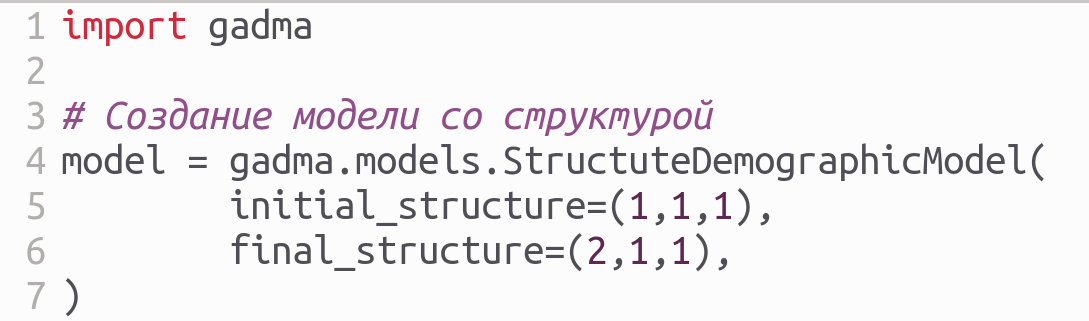
\includegraphics[width=0.6\linewidth]{images/gadma_model_str.png}
% %     \caption{Пример задания струкурной модели демографической истории двух популяций с использованием GADMA}
% %     \label{fig:gadma_model_str}
% % \end{figure}

% \begin{table}[h]
%     \centering
%     \resizebox{\linewidth}{!}{%
%     \begin{tabular}{|l|l|l|}
%         \hline
%          & Задание модели & Условия, накладываемые на элементы \\
%         \hline
%         \dadi & Последовательность & 1. $\mathcal{E}_i \in \mathcal{T}^1 \Leftrightarrow \mathcal{E}_{i-1} \in \mathcal{T}^1 $\\
%         & временных интервалов & 2. $\mathcal{E}_i \in \mathcal{S}^{1,1} \Leftrightarrow \mathcal{E}_{i-1} \in \mathcal{T}^1 \text{ и } \mathcal{E}_{i+1} \in \mathcal{T}^1 \cup \mathcal{S}^{2,1} \cup \mathcal{S}^{2,2}$\\
%         & и разделений: & 3. $\mathcal{E}_i \in \mathcal{T}^2 \Leftrightarrow \mathcal{E}_{i-1} \in \mathcal{T}^2 \cup \mathcal{S}^{1,1}$\\
%         & $\{\mathcal{E}_i\}_{i=1}^E,\ \mathcal{E}_i \in \mathcal{M}_{\text{\dadi}}$ & 4. $\mathcal{E}_i \in \mathcal{S}^{2,1} \cup \mathcal{S}^{2,2} \Leftrightarrow \mathcal{E}_{i-1} \in \mathcal{T}^2 \cup \mathcal{S}^{1,1} \text{ и } \mathcal{E}_{i+1} \in \mathcal{T}^3$\\
%         & & 5. $\mathcal{E}_i \in \mathcal{T}^3 \Leftrightarrow \mathcal{E}_{i-1} \in \mathcal{T}^3 \cup \mathcal{S}^{2,1} \cup \mathcal{S}^{2,2}$ \\
%         \hline
%         \moments & Последовательность & 1. $\mathcal{E}_i \in \mathcal{S}^{\text{\moments}} \Leftrightarrow p_{i} \leq d_j,$\\
%         & временных интервалов & $\text{ где } j=\max\left\{k\in \{1, \dots, i\}:\ \mathcal{E}_k \in \mathcal{T}^{\text{\moments}}\right\} $\\
%         & и разделений: & \\
%         & $\{\mathcal{E}_i\}_{i=1}^E,\ \mathcal{E}_i \in \mathcal{T}^{\text{\moments}} \cup \mathcal{S}^{\text{\moments}}$ & \\
%         \hline
%         \momi & Дерево с расстояниями & 1. $\forall p_i:\ \mathcal{E}_i \in V_{dim=2}\ \exists j:\ \mathcal{E}_j \in V_{dim=1}$\\
%         & в виде элементов: & 2. $\forall p^{to}_i:\ \mathcal{E}_i \in V_{dim=3}\ \exists j:\ \mathcal{E}_j \in V_{dim=1}$\\
%         & $\{\mathcal{E}_i\}_{i=1}^E,\ $ & 3. $\forall p^{from}_i:\ \mathcal{E}_i \in V_{dim=3}\ \exists j:\ \mathcal{E}_j \in V_{dim=1}$\\
%         & $\mathcal{E}_i \in V_{dim=1} \cup V_{dim=2} \cup V_{dim=3}$ & 4. $\mathcal{E}_i \in V_{dim=3}\ \Leftrightarrow \nexists j:\ \mathcal{E}_j \in V_{dim=2} \text{ и } t_j \geq t_i$\\
%         \hline
%         Новая  & Последовательность & 1. $\mathcal{E}_i \in \mathcal{S} \Leftrightarrow p_{i} \leq d_j,$\\
%         модель & временных интервалов & $\text{ где } j=\max\left\{k\in \{1, \dots, i\}:\ \mathcal{E}_k \in \mathcal{T}\right\} $\\
%         & и разделений: & \\
%         & $\{\mathcal{E}_i\}_{i=1}^E,\ \mathcal{E}_i \in \mathcal{T} \cup \mathcal{S}$ & \\
%         \hline
%         % Новая  & Структура & 1. $d_i \leq 3,\ \forall i$\\
%         % модель & $\{s_1, s_2, s_3\}$ & 2. $s_1 \geq 1 $\\
%         % со структ.& &\\
%         % \hline
%     \end{tabular}%
%     }
%     \caption{Способ и условия задания разных моделей ($\mathcal{M}_\text{\dadi} = \mathcal{T}^1 \cup \mathcal{T}^2 \cup \mathcal{T}^3 \cup \mathcal{S}^{1,1} \cup \mathcal{S}^{2,1} \cup \mathcal{S}^{2,2}$)}
%     \label{tab:conditions}
% \end{table}


% \subsubsection{Демографическая история популяций}
% \definition
% \textit{Генетическая популяция} $\mathcal{P}^p$, проиндексированная номером $p$ --- это множество, состоящее из индекса популяции-предка $\mathcal{P}^{parent(p)}$, от которой произошло образование $t^p$ времени назад, времени $t^p > 0$ образования популяции и функции изменения численности $g^p(t),\ t \in [0, t^p]$:
% $$\mathcal{P}^p = \{parent(p), t^p, g^p(t)\},$$
% при условиях:
% $$parent(p) \neq p$$
% $$parent(p) = \emptyset \Longleftrightarrow t^p = \infty$$
% $$t^{parent(p)} > t^p,\quad \forall p$$

% \definition
% \textit{Демографическая история популяций} $\mathfrak{D}$ --- набор генетических популяций:
% $$\mathfrak{D} = \{\mathcal{P}^p\}_{p=1}^K$$
% при дополнительном условии:
% $$parent(p) \in [1, \dots, K]$$

% \subsubsection{Существующие модели демографической истории}

% \textbf{Модель в \dadi.} представляет собой последовательность временных интервалов и разделений популяций.
% Для каждого временного интервала задается его продолжительность, а также функция изменения численности.
% Модель содержит множество элементов, специфичных для числа популяций, что приводит к большому числу условий на задание модели.
% Задание функции изменения численности дополнительно приводит к ошибкам при задании конфигурации модели.


% Элементы модели описаны в таблице~\ref{tab:dadi}, а условия, накладываемые на элементы модели, в таблице~\ref{tab:conditions}.
% Пример задания модели демографической истории популяций для \dadi показан на рисунке~\ref{fig:dadi_model}.

% \begin{table}[h]
%     \centering
%     \begin{tabular}{|l|c|l|}
%         \hline
%         Элементы модели & Обозначение & Параметры элемента \\
%         \hline
%         Временной интервал  & $\mathcal{E}_i \in \mathcal{T}^1$ & 1. Время $t_i$ интервала, \\
%         для одной популяции & & 2. Функция изменения численности \\
%         & & популяции $g_i(t):\ [0, t_i] \to \mathbb{R}_{>0}$. \\
%         \hline
%         Временной интервал & $\mathcal{E}_i \in \mathcal{T}^2$ & 1. Время $t_i$ интервала, \\
%         для двух популяций & & 2. Функция изменения численности \\
%         & & первой популяции $g^1_i(t):\ [0, t_i] \to \mathbb{R}_{>0}$, \\
%         & & 3. Функция изменения численности \\
%         & & второй популяции $g^2_i(t):\ [0, t_i] \to \mathbb{R}_{>0}$. \\
%         \hline
%         Временной интервал & $\mathcal{E}_i \in \mathcal{T}^3$ & 1. Время $t_i$ интервала, \\
%         для трех популяций & & 2. Функция изменения численности \\
%         & & первой популяции $g^1_i(t):\ [0, t_i] \to \mathbb{R}_{>0}$, \\
%         & & 3. Функция изменения численности \\
%         & & второй популяции $g^2_i(t):\ [0, t_i] \to \mathbb{R}_{>0}$. \\
%         & & 3. Функция изменения численности \\
%         & & третьей популяции $g^3_i(t):\ [0, t_i] \to \mathbb{R}_{>0}$. \\
%         \hline
%         Разделение первой & $\mathcal{E}_i \in \mathcal{S}^{1,1}$ & $\emptyset$ \\
%         поп. при условии & & \\
%         одной популяции  & & \\
%         \hline
%         Разделение первой & $\mathcal{E}_i \in \mathcal{S}^{2,1}$ & $\emptyset$ \\
%         поп. при условии & & \\
%         двух популяций  & & \\
%         \hline
%         Разделение второй & $\mathcal{E}_i \in \mathcal{S}^{2,2}$ & $\emptyset$ \\
%         поп. при условии & & \\
%         двух популяций  & & \\
%     \hline
%     \end{tabular}
%     \caption{Элементы модели и их параметры в \dadi}
%     \label{tab:dadi}
% \end{table}

% \begin{figure}[h]
%     \centering
%     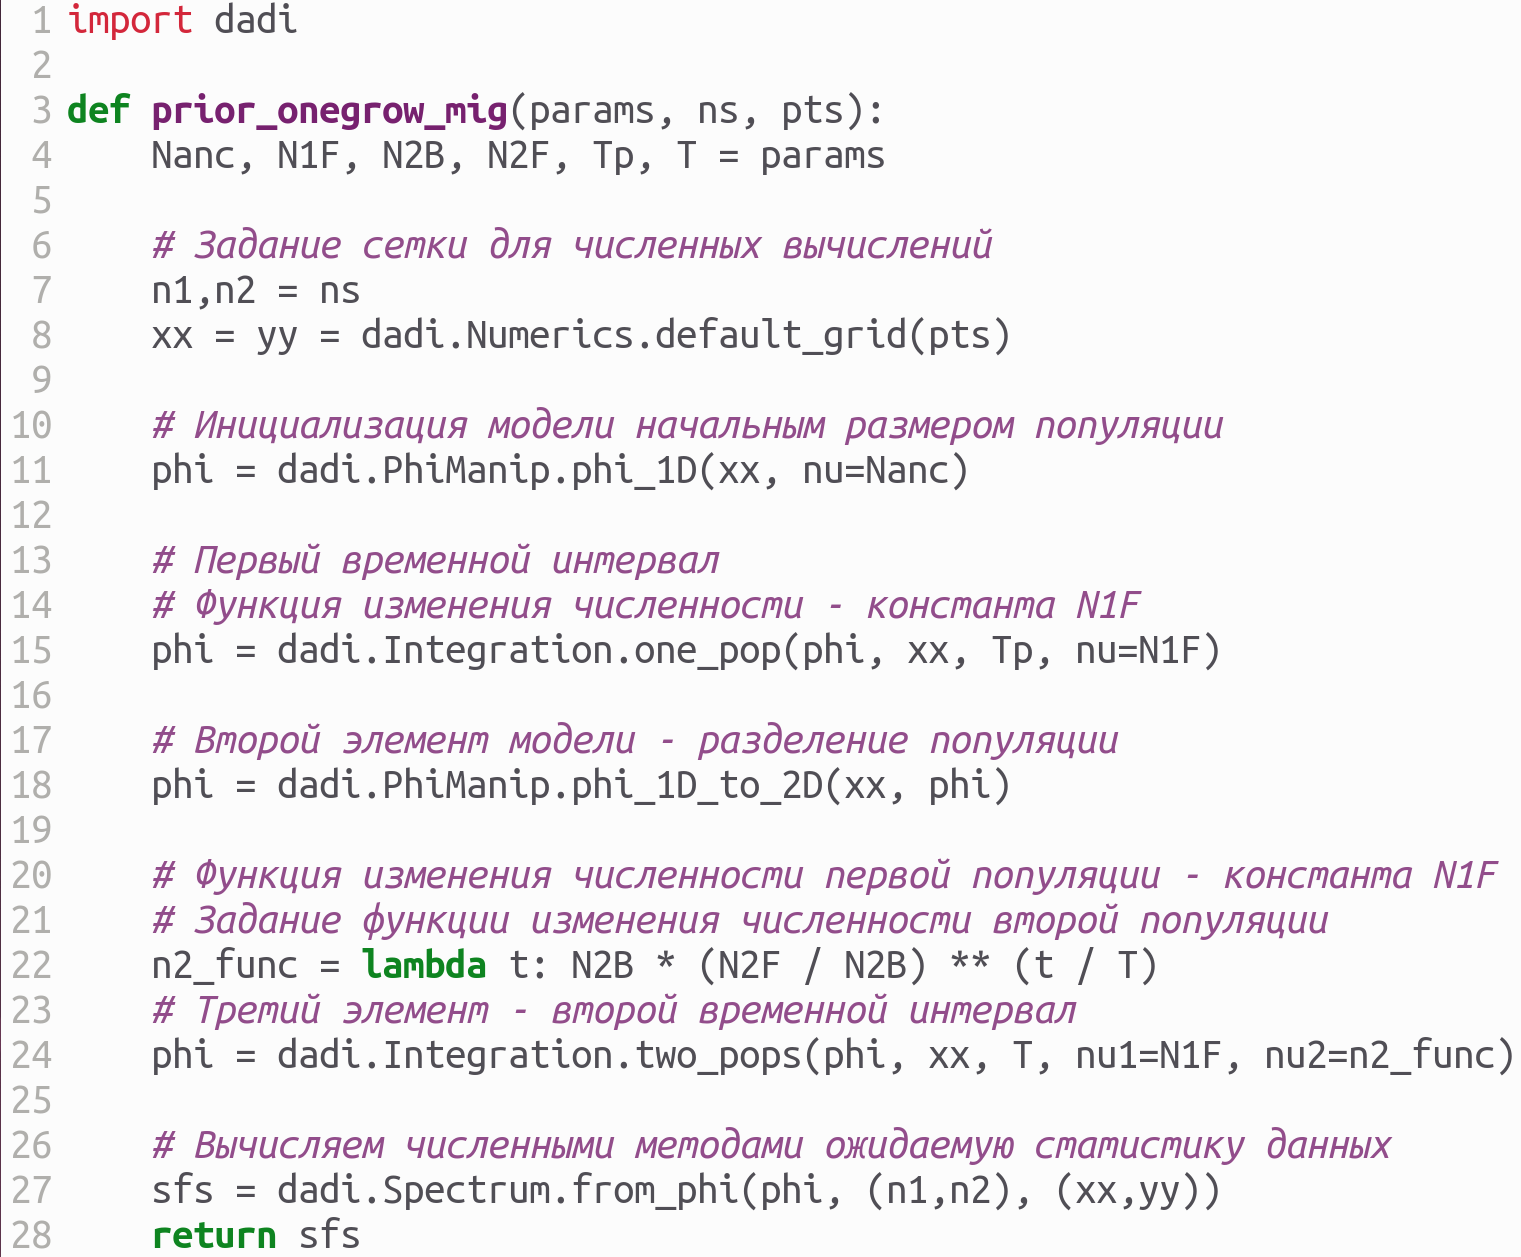
\includegraphics[width=0.6\linewidth]{images/dadi_model.png}
%     \caption{Пример задания модели демографической истории двух популяций с использованием библиотеки \dadi}
%     \label{fig:dadi_model}
% \end{figure}

% Модель $\{\mathcal{E}_i\}_{i=1}^E$ в \dadi задает следующую демографическую историю популяций.
% Число $K$ генетических популяций $\{\mathcal{P}^p\}_{p=1}^K$ определяется по последнему элементу $\mathcal{E}_E$ следующим образом:
% $$
% K = 
% \begin{cases}
%     1, & \text{ если } \mathcal{E}_E \in \mathcal{T}^1 \\
%     2, & \text{ если } \mathcal{E}_E \in \mathcal{S}^{1,1} \cup \mathcal{T}^2 \\
%     3, & \text{ если } \mathcal{E}_E \in \mathcal{S}^{2,1} \cup \mathcal{S}^{2,2} \cup \mathcal{T}^3 \\
% \end{cases}
% $$

% Индекс популяции-предка $parent(p)$ каждой $\mathcal{P}^p$ будет определяться следующим образом:
% $$
% parent(p) = 
% \begin{cases}
%     \emptyset, & \text{ если } p=1\\
%     1, & \text{ если } p=2\\
%     1, & \text{ если } p=3 \text{ и } \exists i: \mathcal{E}_i \in \mathcal{S}^{2,1}\\
%     2, & \text{ если } p=3 \text{ и } \exists i: \mathcal{E}_i \in \mathcal{S}^{2,2}\\
% \end{cases}
% $$

% Время образования $t^p$ популяции $\mathcal{P}^p$ равно:
% $$
% t^p = 
% \begin{cases}
%     \infty, & \text{ если } p=1, \\
%     \sum{t_i}, \text{ для } \forall i:\ \mathcal{E}_i \in T^2,& \text{ если } p=2, \\
%     \sum{t_i}, \text{ для } \forall i:\ \mathcal{E}_i \in T^3,& \text{ если } p=3. \\
% \end{cases}
% $$

% Функция изменения численности определяется функциями, заданными на интервалах.


% \textbf{Модель в \moments} (и в \momentsLD) представляет собой также последовательность временных интервалов и разделений популяций.
% Однако элемент временного интервала един для любого числа популяций.
% Следовательно, задание модели в \moments более универсально, чем в \dadi.
% Однако все также требует прописанной функции изменения численности, что потенциально приводит к ошибкам в спецификации.

% \begin{table}[h]
%     \centering
%     \begin{tabular}{|l|c|l|}
%         \hline
%         Элементы модели & Обозначение & Параметры элемента \\
%         \hline
%         Временной интервал  & $\mathcal{E}_i \in \mathcal{T}^{\text{\moments}}$ & 1. Время $t_i$ интервала, \\
%         & & 2. Функция изменения численности \\
%         & & популяции $g_i(t):\ [0, t_i] \to \mathbb{R}^{d_i}_{>0}$, \\
%         & & где $d_i$ --- число популяций в интервале.\\
%         \hline
%         Разделение & $\mathcal{E}_i \in \mathcal{S}^{\text{\moments}}$ & 1. Индекс $p_i$, разделяемой популяции\\
%         популяции & & \\
%     \hline
%     \end{tabular}
%     \caption{Элементы модели и их параметры в \moments и \momentsLD}
%     \label{tab:moments}
% \end{table}

% \begin{figure}[h]
%     \centering
%     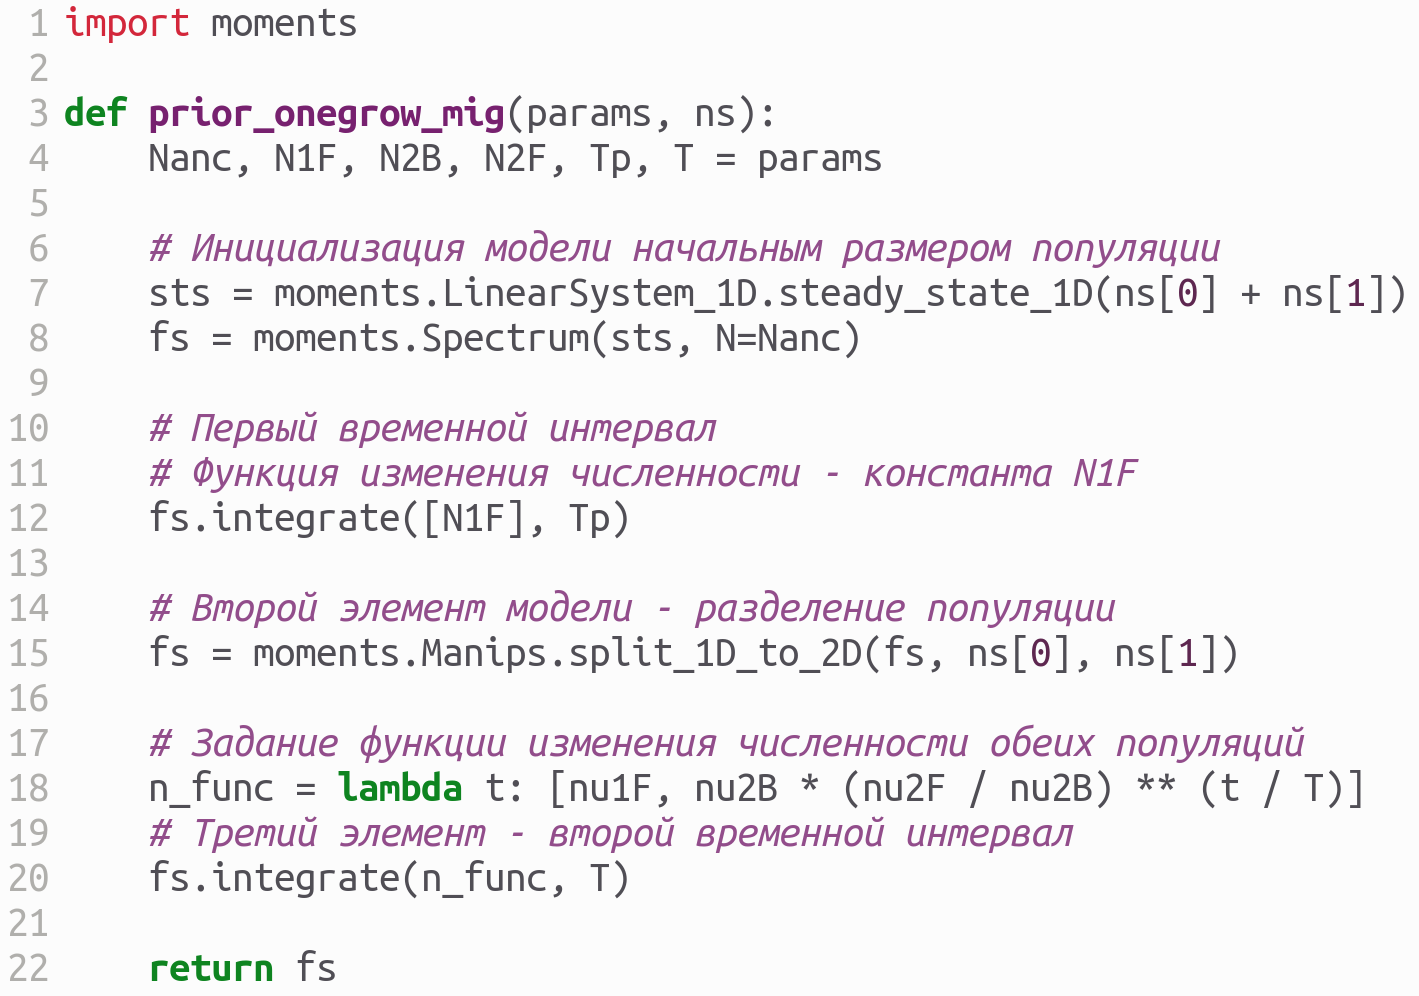
\includegraphics[width=0.6\linewidth]{images/moments_model.png}
%     \caption{Пример задания модели демографической истории двух популяций с использованием библиотеки \moments}
%     \label{fig:dadi_model}
% \end{figure}

% Модель $\{\mathcal{E}_i\}_{i=1}^E$ в \moments задает следующую демографическую историю популяций.
% Число $K$ генетических популяций $\{\mathcal{P}^p\}_{p=1}^K$ определяется по последнему элементу $\mathcal{E}_E$ следующим образом:
% $$K = d_E$$

% Индекс популяции-предка $parent(p)$ каждой $\mathcal{P}^p$:
% $$
% parent(p) =
% \begin{cases}
% \infty, & \text{ если } p = 1, \\
% p_i,\ i:\ \mathcal{E}_i \in \mathcal{S}^{\moments} \text{ и } d_j = p - 1, & \text{ в противном случае,}\\
% \end{cases}
% $$

% где $j = \max \{k \in \{1, \dots, i\}:\ \mathcal{E}_k \in \mathcal{T}\}$.

% Время образования $t^p$ популяции $\mathcal{P}^p$ равно:
% $$
% t^p = 
% \begin{cases}
%     \infty, & \text{ если } p=1, \\
%     \sum{t_i}, \text{ для } \forall i:\ \mathcal{E}_i \in \mathcal{T}^{\moments} \text{ и } d_i = 2,& \text{ если } p=2, \\
%     \sum{t_i}, \text{ для } \forall i:\ \mathcal{E}_i \in \mathcal{T}^{\moments} \text{ и } d_i = 2,& \text{ если } p=3. \\
% \end{cases}
% $$

% Функция изменения численности определяется функциями, заданными на интервалах.

% \textbf{Модель в \momi} представляется в виде множества графов $\{G=(V, E)\}$ популяций.
% В силу особенностей объекта демографической истории каждый граф является деревом.
% Множество деревьев задается тремя элементами: 1) листьями, которые соответствуют популяциям в настояший момент; 2) промежуточными вершинами степени 2, которые соответствуют изменению численности популяции и 3) вершинами размерности 3, которые определяют топологию филогенетического дерева, то есть разделения популяций.
% У каждой вершины дерева, кроме листьев определено расстояние до соответствующего листа-популяции.

% В целях использования функции экспоненциального изменения численности популяций в модели \momi присутствуют параметры степени экспоненциального изменения популяции.
% Параметр $r_p$ определяет следующую функцию изменения численности:
% $$g^p(t) = N_p \cdot e^{-r_p \cdot t}$$

% У каждого дерева $T = (V, E) \in G$ будут определены две функции на множестве ребер $E$.
% Первая функция $ind:\ E \to \{p_i\}$ --- функция, ставящая ребру $e$ индекс популяции в соответствие:
% $$
% ind(e=(v_i, parent(v_i))) = 
% \begin{cases}
% p^{to}_i, & \text{ если } v_i \in V_{dim=3}, \\
% p_i, & \text{ если } v_i \in V_{dim=1} \cup V_{dim=2}, \\
% \end{cases}
% $$
% Вторая функция $dist$ --- функция расстояния, которая определяется временем разделений и изменений численности.

% $$dist(e=(v_i, v_j=parent(v_i))) =
% \begin{cases}
% t_i, & \text{ если } v_i \in V_{dim=1}, \\
% t_{j} - t_{i}, & \text{ если } v_i \in V_{dim=2} \cup V_{dim=3}, \\
% \end{cases}
% $$

% На рисунке~\ref{fig:momi_model}б изображены два дерева, соответствующие модели \momi.
% Красным цветом отмечены ребра $e$, у которых $ind(e) = 1$, то есть они соответствуют первой популяции.
% Черные ребра отображают значение $ind(e) = 1$.
% Значения функции расстояний $dist$ отображено значениями на ребрах.


% \begin{table}[t]
%     \centering
%     \begin{tabular}{|l|c|l|}
%         \hline
%         Элементы модели & Обозначение & Параметры элемента \\
%         \hline
%         Лист популяции  & $\mathcal{E}_i \in V_{dim=1}$ & 1. Индекс $p_i$ популяции\\
%         & & 2. Размер популяции $N_{p_i} \in \mathbb{R}_{>0}$\\
%         & & 3. Степень экспоненциального \\
%         & & изменения популяции $r_{p_i} \in \mathbb{R}$.\\
%         \hline
%         Изменение   & $\mathcal{E}_i \in V_{dim=2}$ & 1. Индекс $p_i$ популяции\\
%         численности & & 2.  Время изменения $t_i \in \mathbb{R}_{>0}$ \\
%         популяции   & & 3.  Размер популяции $N_{p_i} \in \mathbb{R}_{>0}$ \\
%         & & 4. Степень экспоненциального\\
%         & & изменения популяции $r_{p_i} \in \mathbb{R}$. \\
%         \hline
%         Слияние   & $\mathcal{E}_i \in V_{dim=3}$ & 1. Время образования $t_i \in \mathbb{R}_{>0}$\\
%         популяции  & & 2. Индекс $p^{to}_i$ популяции-предка\\
%          & & 3.  Индекс $p^{from}_i$ образованной популяции \\
%     \hline
%     \end{tabular}
%     \caption{Элементы модели и их параметры в \momi. По сравнению с \dadi и \moments время в модели идет в противоположную сторону: от настоящего в прошлое. Поэтому разделение популяции представляется как слияние}
%     \label{tab:moments}
% \end{table}

% \begin{figure}[h]
%     \centering
%     \begin{subfigure}[c]{.57\textwidth}
%     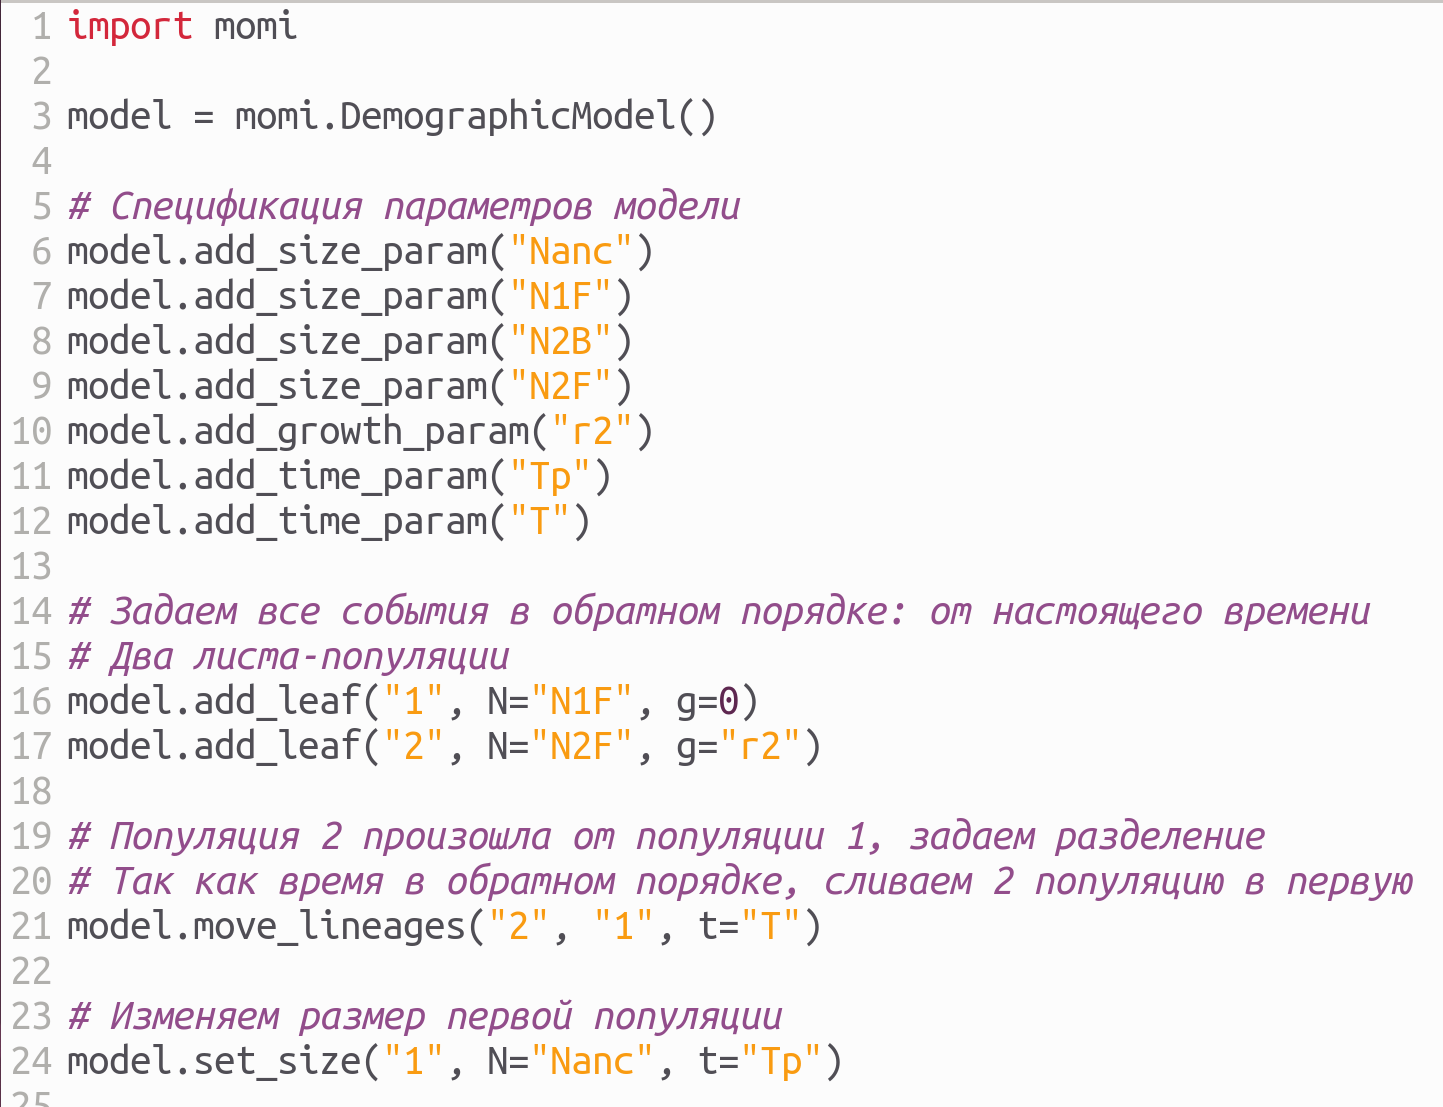
\includegraphics[width=\textwidth]{images/momi_model.png}
%     \caption{}
%     \end{subfigure}%
%     \begin{subfigure}[c]{.4\textwidth}
%     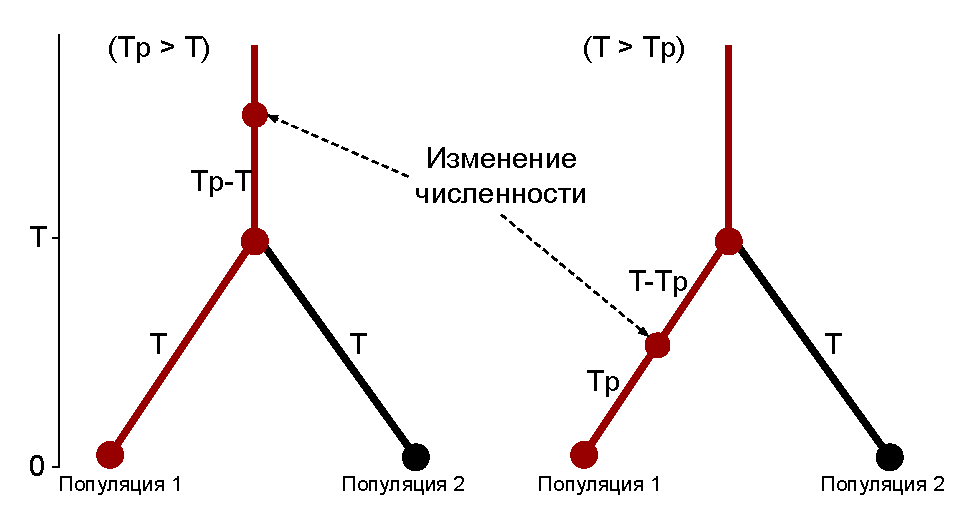
\includegraphics[width=\textwidth]{images/momi_graphs.pdf}
%     \caption{}
%     \end{subfigure}
%     \caption{Пример задания модели демографической истории двух популяций с использованием библиотеки \momi, а также набор деревьев, который ей соответсвует}
%     \label{fig:momi_model}
% \end{figure}

% Модель в \momi с заданными параметрами будет описывать один вариант дерева $T = (V, E)$ из множества $G$, который будет соответствовать следующей демографической истории.
% Размер множества генетических популяций определяется числом листьев:
% $$K=\#\{\mathcal{E}_i:\ \mathcal{E}_i \in V_{dim=1}\}.$$
% Индекс популяции-предка и время образования популяции $\mathcal{P}^p$:
% \begin{align*}
%     parent(p) & = p^{to}_j, \\
%     t^p & =  t_j,
% \end{align*}
% где  $j: \mathcal{E}_j \in V_{dim=3} \text{ и } p^{from}_j = p$.



% \subsubsection*{Предложенная расширенная модель}

% Мы предлагаем новую математическую модель для описания демографической истории популяций.
% Модель расширена наличием таких параметров как динамики изменения численности $D_{i,p}$, которые до этого никогда не включали в модели.
% Эта модель основана на модели \moments.
% Параметр динамики дискретный: принимает значение из области определения, которая по умолчанию использована как $\{const, lin, exp\}$ и соответствует трем функциям изменения численности:
% $$
% g^p_i(t) = 
% \begin{cases}
%     N^{end}_{i,p},& \text{ если } D_{i,p} = const,\\
%     N^{end}_{i,p} + (N^{start}_{i,p} - N^{end}_{i,p})\cdot \frac{t}{t_i},& \text{ если } D_{i,p} = lin,\\
%     N^{end}_{i,p} \cdot (\frac{N^{start}_{i,p}}{N^{end}_{i,p}})^\frac{t}{t_i},& \text{ если } D_{i,p} = exp,\\
% \end{cases}
% $$
% где $t_i$, $N^{start}_p$, $N^{end}_p$ --- параметры продолжительности временного интервала, численности популяции в начале и в конце интервала соответственно.
% Если взять $g_i(t) = (g^1_i(t), \dots, g^K_i(t))$, то модель сведена к модели \moments, для которой описание соответствующей демографической истории уже было дано.

% \begin{table}[h]
%     \centering
%     \begin{tabular}{|l|c|l|}
%         \hline
%         Элементы модели & Обозначение & Параметры элемента \\
%         \hline
%         Временной интервал  & $\mathcal{E}_i \in \mathcal{T}$ & 1. Время $t_i$ интервала, \\
%          & & 2. Размер популяций $\{N^{start}_{i,p}\}_{p=1}^{d_i}$ в начале\\
%         & & интервала, где $d_i$ --- число популяций.\\
%          & & 3. Размер популяций $\{N^{end}_{i,p}\}_{p=1}^{d_i}$ в конце\\
%         & & интервала, где $d_i$ --- число популяций.\\
%         & & 4. Динамики изменения численности\\
%         & & $\{D_{i,p}\}_{p=1}^{d_i}$, $D_{i,p} \in \{const, lin, exp\}$.\\
%         \hline
%         Разделение & $\mathcal{E}_i \in \mathcal{S}$ & 1. Индекс $p_i$, разделяемой популяции,\\
%         популяции & & 2. Отношение $f_i$, в котором разделяется \\
%         & & численность популяции\\
%     \hline
%     \end{tabular}
%     \caption{Элементы и их параметры новой разработанной расширенной модели}
%     \label{tab:moments}
% \end{table}

% \begin{figure}[h]
%     \centering
%     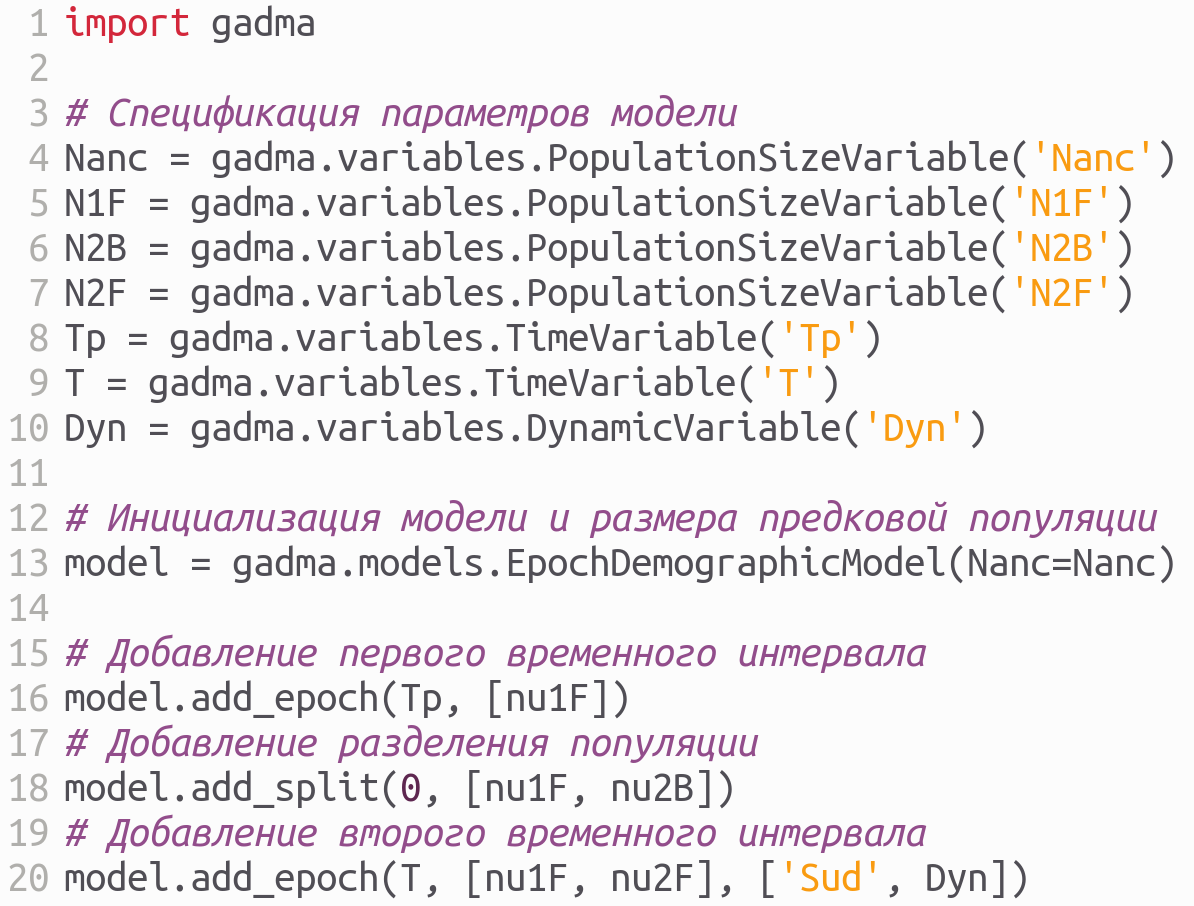
\includegraphics[width=0.6\linewidth]{images/gadma_model.png}
%     \caption{Пример задания новой расширенной модели демографической истории двух популяций с использованием программного комплекса GADMA}
%     \label{fig:dadi_model}
% \end{figure}


% \subsubsection*{Способ задания модели через структуру}


% Также была предложена новый способ задания модели через структуру --- набора чисел, который определяет число временных интервалов в предложенной модели демографической истории.
% Параметры динамик определяют функции изменения численности и могут принимать одно из трех возможных значений $D^p_i \in \{const, lin, exp\}$, которые соответствуют константной численности, линейному изменению и экспоненциальному изменению соответственно.

% Модель описывается заданием структуры $S=\{s_i\},\ i = 1, \dots P$, где $P \in \{1, 2, 3\}$ --- число популяций, $s_1 \geq 1$, $s_1 \geq 0$, $s_1 \geq 0$ соответствуют числу временных интервалов до первого разделения, между первым и вторым и после второго разделения.
% При этом, если $s_2 = 0$, то $s_3 = 0$.

% Таким образом модель со структурой $\{s_1, s_2, s_3\}$ задает следующую модель демографической истории:
% $$\{\mathcal{E}_i\}_{i=1}^{K},$$
% где число элементов $K$ задается:
% $$
% K = 
% \begin{cases}
%     s_1, & \text{ если } s_2 = 0 \text{ и } s_3 = 0, \\
%     s_1 + s_2 + 1, & \text{ если } s_2 > 0 \text{ и } s_3 = 0, \\
%     s_1 + s_2 + s_3 + 2, & \text{ если } s_2 > 0 \text{ и } s_3 > 0, \\
% \end{cases}
% $$

% Каждый элемент $\mathcal{E}_i$ конфигурации модели является:
% $$
% \mathcal{E}_i \in 
% \begin{cases}
%     \mathcal{S}, & \text{ если } i = s_1 \text{ или } i = s_1 + s_2 + 1, \\
%     \mathcal{T}, & \text{ в противном случае }. \\
% \end{cases}
% $$

% Модель имеет следующий набор параметров:
% \begin{align*}
% \theta = &\{t_i\}_{i=2}^{\sum s_j} \cup \\
% & \{N^1_i\}_{i=1}^{s_1+s_2+s_3} \cup \{N^2_i\}_{i=1}^{s_2+s_3} \cup \{N^3_i\}_{i=1}^{s_3} \cup\\
% & \{D^1_i\}_{i=2}^{s_1+s_2+s_3} \cup \{D^2_i\}_{i=1}^{s_2+s_3} \cup \{D^3_i\}_{i=1}^{s_3} \cup \\
% & \theta_{additional},
% \end{align*}
% где множество параметров $\theta_{additional}$ отличается от заданной структуры и определяется следующим образом:
% $$
%   \theta_{additional} =
%   \begin{cases}
%     \emptyset, & \text{если } s_2 = 0, s_3 = 0 \\
%     \{f_1\}, & \text{если } s_2 > 0, s_3 = 0 \\
%     \{f_1, f_2\}, & \text{если } s_2 > 0, s_3 > 0
%   \end{cases}
% $$

% Определим объекты, которые определяют параметры модели и опишем демографическую историю $\mathfrak{D}$, заданную моделью со структурой $\{s_1, s_2, s_3\}$.
% Множество генетических популяций демографической истории будет следующим:
% $$\mathcal{P} = 
% \begin{cases}
%     \{\mathcal{P}^1\}, & \text{если } s_2 = 0, s_3 = 0 \\
%     \{\mathcal{P}^1, \mathcal{P}^2\}, & \text{если } s_2 > 0, s_3 = 0 \\
%     \{\mathcal{P}^1, \mathcal{P}^2, \mathcal{P}^3\}, & \text{если } s_2 > 0, s_3 > 0
% \end{cases}
% $$

% Напомним, что каждая генетическая популяция $\mathcal{P}^p$ --- это пара предковой популяции $\mathcal{P}^p_{parent}$ и упорядоченного множества эпох $\{\mathcal{E}^p_j\}_{j=1}^{E_p}$.
% Наша модель определяет предковые популяции $\mathcal{P}^p_{parent}$ следующим образом:
% $$\mathcal{P}^p_{parent} = 
% \begin{cases}
%     \emptyset, & \text{если } p=1 \\
%     \mathcal{P}^1, & \text{если } p=2 \\
%     \mathcal{P}^2, & \text{если } p=3
% \end{cases}
% $$
% Каждая эпоха --- это множество $\mathcal{E}^p_j = \{t^{p,j}_{start}, t^{p,j}_{end}, g^p_j(t)\}$, где $t^{p,j}_{start}, t^{p,j}_{end} \in \mathbb{R}_{>0}$ соответствуют времени начала эпохи и конца, функция $g^p_j(t)$ определяет численность популяции $\mathcal{P}^p$ в момент времени $t \in [t^{p,j}_{start}, t^{p,j}_{end}]$.
% Также на времена начала и конца эпох наложены следующие условия; $t^{p,j}_{start} > t^{p,j}_{end}$, а $t^{p,j-1}_{end} = t^{p,j}_{start}$.

% Модель со структурой $s_1, s_2, s_3$ будет содержать следующее число эпох для каждой популяции $\mathcal{P}^p$:
% $$E_p = 
% \begin{cases}
%     s_1 + s_2 + s_3, & \text{если } p=1 \\
%     s_2 + s_3, & \text{если } p=2 \\
%     s_3, & \text{если } p=3
% \end{cases}
% $$

% Наконец, перейдем к пояснению параметров модели, которые определяют эпохи популяций в демографической истории.
% Параметр $t_j$ задает время продолжительности эпохи $\mathcal{E}^p_j$ для каждой генетической популяции $\mathcal{P}^p$ демографической истории $\mathfrak{D}$, то есть $t_j = t^{p,j}_{start} - t^{p,j}_{ends},\ \forall p = \{1, 2, 3\}$.
% Таким образом модель задает следующие времени начала и окончания эпохи $\mathcal{E}^p_j,\ j \in \{1, \dots, E_p\}$ для популяции $\mathcal{P}^p$:
% $$
% t^{p,j}_{start} =
% \begin{cases}
%     \infty, & \text{если } p=1,\ j=1 \\
%     \sum_{i=1}^{j} t_i, & \text{если } p=1,\ j \geq 2 \\
%     \sum_{i=s_1}^{s_1+j} t_i, & \text{если } p=2 \\
%     \sum_{i=s_1+s_2}^{s_1+s_2+j} t_i, & \text{если } p=3 \\
% \end{cases}
% $$
% Время окончания для эпох можно определить как:
% $$
% t^{p,j}_{end} =
% \begin{cases}
%     t^{p,j + 1}_{start}, & \text{для } \forall j \in \{1, \dots, E_p-1\}\\
%     0, & \text{для }  j = E_p
% \end{cases}
% $$

% Параметр $N^p_i$ задает размер популяции $\mathcal{P}^1$ в конце эпохи $\mathcal{E}^p_j$, то есть $g^p_j(t^{p,j}_{end}) = N^p_i$ а параметр $D^p_i$ определяет функцию изменения численности популяции $\mathcal{P}^1$ во время эпохи $\mathcal{E}^p_j$, $j \geq 2$ как:
% $$g^p_j(t) = 
% \begin{cases}
%     N^p_j, & \text{если } (p=1 и j=1) или D^p_j = constant, \\
%     N^p_{j-1} + \left(N^p_j - N^p_{j, start}\right) \cdot \frac{(t - t^{p,j}_{start})}{t^{p,j}_{end}}, & \text{если } D^p_j = linear, \\
%     N^p_{start} \cdot \left(\frac{N^p_j}{N^p_{j, start}}\right)^{\frac{(t - t^{p,j}_{start})}{t^{p,j}_{end}}}, & \text{если } D^p_j = exponential,
% \end{cases}
% $$
% где $N^p_{j, start}$ равен размеру популяции в начале эпохи.
% Зачастую размер в начале эпохи равен размеру популяции в конце предыдущей эпохи.
% Однако у нас присутствует разделение популяций, имеющие параметры $f_1$ и $f_2$, каждое из которых определяет отношение численности, в котором разделяется предковая популяция.
% Таким образом $N^p_{j, start}$ будет определяться следующим образом:
% $$
% N^1_{j, start} = 
% \begin{cases}
%     N^1_1, & \text{если } j=1, \\
%     N^1_{j-1} \cdot f_1, & \text{если } j=s_1+1, \\
%     N^1_{j-1}, & \text{в противном случае}.
% \end{cases}
% $$
% $$
% N^2_{j, start} = 
% \begin{cases}
%     N^1_{s_1} \cdot (1-f_1), & \text{если } j=1,\\
%     N^2_{j-1} \cdot f_2, & \text{если } j=s_2+1,\\
%     N^2_{j-1}, & \text{в противном случае}.
% \end{cases}
% $$
% $$
% N^3_{j, start} = 
% \begin{cases}
%     N^1_{s_2} \cdot (1-f_2), & \text{если } j=1,\\
%     N^2_{j-1}, & \text{в противном случае}.
% \end{cases}
% $$

%\clearpage\urlstyle{rm}\printbibliography\urlstyle{tt}
\printbibliography[notcategory=skipbibliography]
% \clearpage\listoffigures
% \clearpage\listoftables
\newpage

%%% Настройки для приложений
\appendix
% \counterwithin{figure}{chapter}
% \counterwithin{table}{chapter}
%\counterwithin{algorithm}{chapter}
%\counterwithin{lstlisting}{chapter}
% \renewcommand{\thechapter}{\Asbukx{chapter}}

% \include{Dissertation/appendix}        % Приложения

% \clearpage
% \chapter*{Публикации} \addcontentsline{toc}{chapter}{Публикации}

\begin{refsection}
%\nociteallauthorpublications
%\urlstyle{rm}\printauthorpublicationsappendix\urlstyle{tt}
%\includepdf[pages=-,pagecommand={}]{Papers/*.pdf}
\end{refsection}

\end{document}